\documentclass[manuscript,review]{acmart}
% ACM TACCESS submission skeleton. Build (repo root mounted so ../figs resolves):
%   docker run --rm -v ~/aac-voice-preservation:/w -w /w/paper/journal texlive/texlive:latest-full latexmk -pdf main.tex
% Assembled from sections/s1..s5 (pass 1 integrator). Every number is a \jm... macro from make_macros.py (results_macros.tex). Do not hand-type numbers.
% results_macros.tex -- GENERATED by paper/journal/make_macros.py. Do not edit by hand.
\newcommand{\jmaskBudgetPct}{10}
\newcommand{\jmaskMdePol}{8.5}
\newcommand{\jmaskMdeRelPol}{35.7}
\newcommand{\jmaskPrimaryN}{4}
\newcommand{\jmaskPrimarySig}{0}
\newcommand{\jmaskPriorMinusRandPol}{-4.2}
\newcommand{\jmaskPriorMinusRandPolHi}{2.2}
\newcommand{\jmaskPriorMinusRandPolLo}{-8.5}
\newcommand{\jmaskPriorMinusRandPolite}{-5.6}
\newcommand{\jmaskPriorMinusRandPoliteHi}{2.7}
\newcommand{\jmaskPriorMinusRandPoliteLo}{-16.4}
\newcommand{\jmbmCells}{36}
\newcommand{\jmbmFullMin}{87.6}
\newcommand{\jmbmGemmaActGain}{+36.6}
\newcommand{\jmbmGemmaActWord}{+13.4}
\newcommand{\jmbmGemmaBare}{100.0}
\newcommand{\jmbmGemmaNoLeg}{98.9}
\newcommand{\jmbmGemmaPolGain}{+49.5}
\newcommand{\jmbmIrrelCells}{36}
\newcommand{\jmbmLlamaActGain}{+18.7}
\newcommand{\jmbmLlamaActWord}{+14.9}
\newcommand{\jmbmLlamaBare}{99.0}
\newcommand{\jmbmLlamaNoLeg}{98.4}
\newcommand{\jmbmLlamaPolGain}{+49.0}
\newcommand{\jmbmMinLegendArm}{97.3}
\newcommand{\jmbmNemoActGain}{+37.3}
\newcommand{\jmbmNemoActWord}{$-$3.7}
\newcommand{\jmbmNemoBare}{99.0}
\newcommand{\jmbmNemoNoLeg}{99.5}
\newcommand{\jmbmNemoPolGain}{+50.0}
\newcommand{\jmbmQwenLActGain}{+35.1}
\newcommand{\jmbmQwenLActWord}{+3.0}
\newcommand{\jmbmQwenLBare}{100.0}
\newcommand{\jmbmQwenLNoLeg}{100.0}
\newcommand{\jmbmQwenLPolGain}{+50.0}
\newcommand{\jmbmQwenSActGain}{+35.1}
\newcommand{\jmbmQwenSActWord}{+9.0}
\newcommand{\jmbmQwenSBare}{100.0}
\newcommand{\jmbmQwenSNoLeg}{98.9}
\newcommand{\jmbmQwenSPolGain}{+49.5}
\newcommand{\jmbmTerraActGain}{+50.7}
\newcommand{\jmbmTerraActWord}{$-$4.5}
\newcommand{\jmbmTerraBare}{100.0}
\newcommand{\jmbmTerraNoLeg}{97.3}
\newcommand{\jmbmTerraPolGain}{+50.0}
\newcommand{\jmbmWordEqCells}{27}
\newcommand{\jmbreadthFamilies}{5}
\newcommand{\jmbreadthMinAff}{99.0}
\newcommand{\jmbreadthModels}{6}
\newcommand{\jmbreadthOrigModels}{4}
\newcommand{\jmbreadthPolChipMin}{+49.0}
\newcommand{\jmbreadthSpeechChipMax}{+50.7}
\newcommand{\jmbreadthSpeechChipMin}{+18.7}
\newcommand{\jmclamDiffPol}{0.0}
\newcommand{\jmclamDiffPolHi}{2.2}
\newcommand{\jmclamDiffPolLo}{-3.0}
\newcommand{\jmclamDiffPolite}{1.8}
\newcommand{\jmclamDiffPoliteHi}{4.3}
\newcommand{\jmclamDiffPoliteLo}{-1.1}
\newcommand{\jmclamMdePol}{3.8}
\newcommand{\jmclamPHolmPol}{1.00}
\newcommand{\jmclamPol}{21.2}
\newcommand{\jmclamPolHi}{30.8}
\newcommand{\jmclamPolLo}{13.6}
\newcommand{\jmconsBadN}{4}
\newcommand{\jmconsBadNeitherOkK}{4}
\newcommand{\jmconsBadNotOkK}{3}
\newcommand{\jmconsBadOkK}{0}
\newcommand{\jmconsChipK}{1}
\newcommand{\jmconsExN}{10}
\newcommand{\jmconsGoodN}{3}
\newcommand{\jmconsGoodNeitherOkK}{2}
\newcommand{\jmconsGoodNotOkK}{2}
\newcommand{\jmconsGoodOkK}{1}
\newcommand{\jmconsImpK}{10}
\newcommand{\jmconsImpN}{10}
\newcommand{\jmconsRepN}{3}
\newcommand{\jmconsRepNeitherOkK}{1}
\newcommand{\jmconsRepNotOkK}{0}
\newcommand{\jmconsRepOkK}{2}
\newcommand{\jmconvBoot}{10,000}
\newcommand{\jmconvBootFOne}{2,000}
\newcommand{\jmconvSeed}{20261031}
\newcommand{\jmconvSeedFOne}{20261103}
\newcommand{\jmctlGAct}{+35.3}
\newcommand{\jmctlGActHi}{+40.3}
\newcommand{\jmctlGActLo}{+31.2}
\newcommand{\jmctlGAgent}{+67.3}
\newcommand{\jmctlGAgentHi}{+69.9}
\newcommand{\jmctlGAgentLo}{+64.8}
\newcommand{\jmctlGCert}{+54.0}
\newcommand{\jmctlGCertHi}{+55.3}
\newcommand{\jmctlGCertLo}{+52.4}
\newcommand{\jmctlGPol}{+49.5}
\newcommand{\jmctlGPolHi}{+49.9}
\newcommand{\jmctlGPolLo}{+49.0}
\newcommand{\jmctlGPolite}{+38.2}
\newcommand{\jmctlGPoliteHi}{+39.4}
\newcommand{\jmctlGPoliteLo}{+36.8}
\newcommand{\jmctlGTime}{+82.7}
\newcommand{\jmctlGTimeHi}{+86.0}
\newcommand{\jmctlGTimeLo}{+80.1}
\newcommand{\jmctlIrrelAddAct}{+5.2}
\newcommand{\jmctlIrrelAddActHi}{+10.4}
\newcommand{\jmctlIrrelAddActLo}{+1.6}
\newcommand{\jmctlIrrelAddAgent}{$-$0.6}
\newcommand{\jmctlIrrelAddAgentHi}{+0.6}
\newcommand{\jmctlIrrelAddAgentLo}{$-$1.9}
\newcommand{\jmctlIrrelAddCert}{+6.5}
\newcommand{\jmctlIrrelAddCertHi}{+7.9}
\newcommand{\jmctlIrrelAddCertLo}{+4.9}
\newcommand{\jmctlIrrelAddPol}{+0.0}
\newcommand{\jmctlIrrelAddPolHi}{+0.0}
\newcommand{\jmctlIrrelAddPolLo}{+0.0}
\newcommand{\jmctlIrrelAddPolite}{+0.0}
\newcommand{\jmctlIrrelAddPoliteHi}{+0.0}
\newcommand{\jmctlIrrelAddPoliteLo}{+0.0}
\newcommand{\jmctlIrrelAddTime}{+1.8}
\newcommand{\jmctlIrrelAddTimeHi}{+4.8}
\newcommand{\jmctlIrrelAddTimeLo}{$-$0.7}
\newcommand{\jmctlIrrelAgent}{+67.9}
\newcommand{\jmctlIrrelCert}{+47.6}
\newcommand{\jmctlIrrelPol}{+49.5}
\newcommand{\jmctlOverIrrelAct}{+30.0}
\newcommand{\jmctlOverIrrelActHi}{+33.9}
\newcommand{\jmctlOverIrrelActLo}{+24.6}
\newcommand{\jmctlOverIrrelAgent}{+67.9}
\newcommand{\jmctlOverIrrelAgentHi}{+69.4}
\newcommand{\jmctlOverIrrelAgentLo}{+66.5}
\newcommand{\jmctlOverIrrelCert}{+47.6}
\newcommand{\jmctlOverIrrelCertHi}{+48.6}
\newcommand{\jmctlOverIrrelCertLo}{+46.6}
\newcommand{\jmctlOverIrrelPol}{+49.5}
\newcommand{\jmctlOverIrrelPolHi}{+49.9}
\newcommand{\jmctlOverIrrelPolLo}{+49.0}
\newcommand{\jmctlOverIrrelPolite}{+38.2}
\newcommand{\jmctlOverIrrelPoliteHi}{+39.4}
\newcommand{\jmctlOverIrrelPoliteLo}{+36.8}
\newcommand{\jmctlOverIrrelTime}{+80.9}
\newcommand{\jmctlOverIrrelTimeHi}{+85.4}
\newcommand{\jmctlOverIrrelTimeLo}{+77.2}
\newcommand{\jmctlOverWordAct}{$-$8.2}
\newcommand{\jmctlOverWordActHi}{$-$5.3}
\newcommand{\jmctlOverWordActLo}{$-$12.1}
\newcommand{\jmctlOverWordAgent}{+0.1}
\newcommand{\jmctlOverWordAgentHi}{+0.4}
\newcommand{\jmctlOverWordAgentLo}{+0.0}
\newcommand{\jmctlOverWordCert}{+0.1}
\newcommand{\jmctlOverWordCertHi}{+1.2}
\newcommand{\jmctlOverWordCertLo}{$-$0.6}
\newcommand{\jmctlOverWordPol}{+0.8}
\newcommand{\jmctlOverWordPolHi}{+1.4}
\newcommand{\jmctlOverWordPolLo}{+0.1}
\newcommand{\jmctlOverWordPolite}{$-$2.1}
\newcommand{\jmctlOverWordPoliteHi}{+0.3}
\newcommand{\jmctlOverWordPoliteLo}{$-$4.7}
\newcommand{\jmctlOverWordTime}{+0.5}
\newcommand{\jmctlOverWordTimeHi}{+1.0}
\newcommand{\jmctlOverWordTimeLo}{+0.1}
\newcommand{\jmdesignConsultants}{2}
\newcommand{\jmdesignDims}{7}
\newcommand{\jmdesignRatersPerItem}{3}
\newcommand{\jmdesignSlp}{2}
\newcommand{\jmdpAlwaysCommitPol}{23.9}
\newcommand{\jmdpAlwaysCommitPolHi}{32.5}
\newcommand{\jmdpAlwaysCommitPolLo}{16.0}
\newcommand{\jmdpAskPriorPol}{17.1}
\newcommand{\jmdpAskPriorPolHi}{28.8}
\newcommand{\jmdpAskPriorPolLo}{10.0}
\newcommand{\jmdpAskRandPol}{21.3}
\newcommand{\jmdpAskRandPolHi}{28.9}
\newcommand{\jmdpAskRandPolLo}{14.2}
\newcommand{\jmdpMdePol}{8.5}
\newcommand{\jmexActBareWrong}{56.0}
\newcommand{\jmexActBareWrongHi}{63.0}
\newcommand{\jmexActBareWrongLo}{52.1}
\newcommand{\jmexActFamilies}{66}
\newcommand{\jmexActRepair}{75.3}
\newcommand{\jmexActRepairHi}{83.2}
\newcommand{\jmexActRepairLo}{66.0}
\newcommand{\jmexActRepairN}{300}
\newcommand{\jmexPolBareN}{832}
\newcommand{\jmexPolBareWrong}{49.8}
\newcommand{\jmexPolBareWrongHi}{50.0}
\newcommand{\jmexPolBareWrongLo}{49.5}
\newcommand{\jmexPolChip}{99.3}
\newcommand{\jmexPolChipHi}{99.8}
\newcommand{\jmexPolChipLo}{98.6}
\newcommand{\jmexPolChipMatch}{99.3}
\newcommand{\jmexPolChipMatchHi}{99.8}
\newcommand{\jmexPolChipMatchLo}{98.6}
\newcommand{\jmexPolChipMatchN}{414}
\newcommand{\jmexPolChipN}{414}
\newcommand{\jmexPolFamilies}{104}
\newcommand{\jmexPolQual}{104}
\newcommand{\jmexPolRepair}{99.3}
\newcommand{\jmexPolRepairHi}{99.8}
\newcommand{\jmexPolRepairLo}{98.6}
\newcommand{\jmexPolRepairN}{414}
\newcommand{\jmexPolWriters}{7}
\newcommand{\jmexPolWrong}{49.8}
\newcommand{\jmexPolWrongHi}{50.0}
\newcommand{\jmexPolWrongLo}{49.5}
\newcommand{\jmexPolWrongN}{832}
\newcommand{\jmexPoliteBareWrong}{50.0}
\newcommand{\jmexPoliteBareWrongHi}{50.0}
\newcommand{\jmexPoliteBareWrongLo}{50.0}
\newcommand{\jmexPoliteFamilies}{89}
\newcommand{\jmexPoliteRepair}{82.0}
\newcommand{\jmexPoliteRepairHi}{84.6}
\newcommand{\jmexPoliteRepairLo}{79.5}
\newcommand{\jmexPoliteRepairN}{356}
\newcommand{\jmfOneActRestoreBare}{29.9}
\newcommand{\jmfOneActRestoreBareHi}{38.6}
\newcommand{\jmfOneActRestoreBareLo}{21.9}
\newcommand{\jmfOneActRestoreChip}{75.6}
\newcommand{\jmfOneActRestoreChipG}{90.4}
\newcommand{\jmfOneActRestoreChipGHi}{94.9}
\newcommand{\jmfOneActRestoreChipGLo}{85.6}
\newcommand{\jmfOneActRestoreChipHi}{81.7}
\newcommand{\jmfOneActRestoreChipLo}{69.8}
\newcommand{\jmfOneActRestoreWord}{79.2}
\newcommand{\jmfOneActRestoreWordHi}{86.0}
\newcommand{\jmfOneActRestoreWordLo}{72.2}
\newcommand{\jmfOneArbRows}{27}
\newcommand{\jmfOneChipMinusWordAct}{$-$3.6}
\newcommand{\jmfOneChipMinusWordActHi}{+1.7}
\newcommand{\jmfOneChipMinusWordActLo}{$-$8.7}
\newcommand{\jmfOneChipMinusWordPol}{+3.9}
\newcommand{\jmfOneChipMinusWordPolHi}{+8.6}
\newcommand{\jmfOneChipMinusWordPolLo}{$-$0.5}
\newcommand{\jmfOneChipMinusWordPolite}{+0.8}
\newcommand{\jmfOneChipMinusWordPoliteHi}{+2.6}
\newcommand{\jmfOneChipMinusWordPoliteLo}{$-$0.9}
\newcommand{\jmfOneDecisionAct}{not distinguishable}
\newcommand{\jmfOneDecisionPol}{not distinguishable}
\newcommand{\jmfOneDecisionPolite}{equivalent}
\newcommand{\jmfOneGuardGainAct}{+14.8}
\newcommand{\jmfOneGuardGainActHi}{+20.1}
\newcommand{\jmfOneGuardGainActLo}{+9.8}
\newcommand{\jmfOneGuardGainPol}{+1.6}
\newcommand{\jmfOneGuardGainPolHi}{+3.3}
\newcommand{\jmfOneGuardGainPolLo}{+0.3}
\newcommand{\jmfOneGuardGainPolite}{+1.2}
\newcommand{\jmfOneGuardGainPoliteHi}{+2.6}
\newcommand{\jmfOneGuardGainPoliteLo}{+0.2}
\newcommand{\jmfOneModels}{3}
\newcommand{\jmfOneRestActBare}{29.9}
\newcommand{\jmfOneRestActBareHi}{38.6}
\newcommand{\jmfOneRestActBareLo}{21.9}
\newcommand{\jmfOneRestActChip}{75.6}
\newcommand{\jmfOneRestActChipG}{90.4}
\newcommand{\jmfOneRestActChipGHi}{94.9}
\newcommand{\jmfOneRestActChipGLo}{85.6}
\newcommand{\jmfOneRestActChipHi}{81.7}
\newcommand{\jmfOneRestActChipLo}{69.8}
\newcommand{\jmfOneRestActWord}{79.2}
\newcommand{\jmfOneRestActWordHi}{86.0}
\newcommand{\jmfOneRestActWordLo}{72.2}
\newcommand{\jmfOneRestPolBare}{2.4}
\newcommand{\jmfOneRestPolBareHi}{5.6}
\newcommand{\jmfOneRestPolBareLo}{0.3}
\newcommand{\jmfOneRestPolChip}{93.4}
\newcommand{\jmfOneRestPolChipG}{95.0}
\newcommand{\jmfOneRestPolChipGHi}{98.6}
\newcommand{\jmfOneRestPolChipGLo}{90.9}
\newcommand{\jmfOneRestPolChipHi}{97.3}
\newcommand{\jmfOneRestPolChipLo}{89.0}
\newcommand{\jmfOneRestPolWord}{89.5}
\newcommand{\jmfOneRestPolWordHi}{94.4}
\newcommand{\jmfOneRestPolWordLo}{84.2}
\newcommand{\jmfOneRestPoliteBare}{8.1}
\newcommand{\jmfOneRestPoliteBareHi}{13.3}
\newcommand{\jmfOneRestPoliteBareLo}{4.1}
\newcommand{\jmfOneRestPoliteChip}{98.8}
\newcommand{\jmfOneRestPoliteChipG}{100.0}
\newcommand{\jmfOneRestPoliteChipGHi}{100.0}
\newcommand{\jmfOneRestPoliteChipGLo}{100.0}
\newcommand{\jmfOneRestPoliteChipHi}{99.8}
\newcommand{\jmfOneRestPoliteChipLo}{97.4}
\newcommand{\jmfOneRestPoliteWord}{97.9}
\newcommand{\jmfOneRestPoliteWordHi}{99.4}
\newcommand{\jmfOneRestPoliteWordLo}{96.1}
\newcommand{\jmfOneRevActBare}{194.5}
\newcommand{\jmfOneRevActBareHi}{216.8}
\newcommand{\jmfOneRevActBareLo}{170.4}
\newcommand{\jmfOneRevActChip}{67.7}
\newcommand{\jmfOneRevActChipG}{26.7}
\newcommand{\jmfOneRevActChipGHi}{39.9}
\newcommand{\jmfOneRevActChipGLo}{14.1}
\newcommand{\jmfOneRevActChipHi}{83.8}
\newcommand{\jmfOneRevActChipLo}{50.7}
\newcommand{\jmfOneRevActWord}{57.7}
\newcommand{\jmfOneRevActWordHi}{77.2}
\newcommand{\jmfOneRevActWordLo}{38.9}
\newcommand{\jmfOneRevPolBare}{23.8}
\newcommand{\jmfOneRevPolBareHi}{24.3}
\newcommand{\jmfOneRevPolBareLo}{23.0}
\newcommand{\jmfOneRevPolChip}{1.6}
\newcommand{\jmfOneRevPolChipG}{1.2}
\newcommand{\jmfOneRevPolChipGHi}{2.2}
\newcommand{\jmfOneRevPolChipGLo}{0.3}
\newcommand{\jmfOneRevPolChipHi}{2.7}
\newcommand{\jmfOneRevPolChipLo}{0.7}
\newcommand{\jmfOneRevPolWord}{2.6}
\newcommand{\jmfOneRevPolWordHi}{3.9}
\newcommand{\jmfOneRevPolWordLo}{1.4}
\newcommand{\jmfOneRevPoliteBare}{51.8}
\newcommand{\jmfOneRevPoliteBareHi}{54.1}
\newcommand{\jmfOneRevPoliteBareLo}{48.9}
\newcommand{\jmfOneRevPoliteChip}{0.7}
\newcommand{\jmfOneRevPoliteChipG}{0.0}
\newcommand{\jmfOneRevPoliteChipGHi}{0.0}
\newcommand{\jmfOneRevPoliteChipGLo}{0.0}
\newcommand{\jmfOneRevPoliteChipHi}{1.4}
\newcommand{\jmfOneRevPoliteChipLo}{0.1}
\newcommand{\jmfOneRevPoliteWord}{1.2}
\newcommand{\jmfOneRevPoliteWordHi}{2.2}
\newcommand{\jmfOneRevPoliteWordLo}{0.3}
\newcommand{\jmfOneUnits}{332}
\newcommand{\jmfOneUnitsAct}{120}
\newcommand{\jmfOneUnitsPol}{76}
\newcommand{\jmfOneUnitsPolite}{136}
\newcommand{\jmgbCDiscGOneMGOner}{+3.2}
\newcommand{\jmgbCDiscGOneMGOnerHi}{+4.8}
\newcommand{\jmgbCDiscGOneMGOnerLo}{+1.9}
\newcommand{\jmgbCDiscGOneMGOnes}{+2.1}
\newcommand{\jmgbCDiscGOneMGOnesHi}{+3.2}
\newcommand{\jmgbCDiscGOneMGOnesLo}{+1.1}
\newcommand{\jmgbCDiscGOneMGOnet}{+0.3}
\newcommand{\jmgbCDiscGOneMGOnetHi}{+0.6}
\newcommand{\jmgbCDiscGOneMGOnetLo}{+0.1}
\newcommand{\jmgbCDiscGOnerMGOnes}{$-$1.1}
\newcommand{\jmgbCDiscGOnerMGOnesHi}{$-$0.3}
\newcommand{\jmgbCDiscGOnerMGOnesLo}{$-$2.1}
\newcommand{\jmgbCDiscGOnetMGOner}{+2.9}
\newcommand{\jmgbCDiscGOnetMGOnerHi}{+4.4}
\newcommand{\jmgbCDiscGOnetMGOnerLo}{+1.7}
\newcommand{\jmgbCDiscGOnetMGOnes}{+1.8}
\newcommand{\jmgbCDiscGOnetMGOnesHi}{+2.7}
\newcommand{\jmgbCDiscGOnetMGOnesLo}{+0.9}
\newcommand{\jmgbCWcGOneMGOner}{+6.2}
\newcommand{\jmgbCWcGOneMGOnerHi}{+7.6}
\newcommand{\jmgbCWcGOneMGOnerLo}{+4.8}
\newcommand{\jmgbCWcGOneMGOnes}{+6.4}
\newcommand{\jmgbCWcGOneMGOnesHi}{+7.5}
\newcommand{\jmgbCWcGOneMGOnesLo}{+5.3}
\newcommand{\jmgbCWcGOneMGOnet}{$-$0.7}
\newcommand{\jmgbCWcGOneMGOnetHi}{+0.1}
\newcommand{\jmgbCWcGOneMGOnetLo}{$-$1.6}
\newcommand{\jmgbCWcGOnerMGOnes}{+0.2}
\newcommand{\jmgbCWcGOnerMGOnesHi}{+1.2}
\newcommand{\jmgbCWcGOnerMGOnesLo}{$-$0.9}
\newcommand{\jmgbCWcGOnetMGOner}{+6.9}
\newcommand{\jmgbCWcGOnetMGOnerHi}{+8.6}
\newcommand{\jmgbCWcGOnetMGOnerLo}{+5.3}
\newcommand{\jmgbCWcGOnetMGOnes}{+7.1}
\newcommand{\jmgbCWcGOnetMGOnesHi}{+8.3}
\newcommand{\jmgbCWcGOnetMGOnesLo}{+6.0}
\newcommand{\jmgbDiscFamilies}{58}
\newcommand{\jmgbDiscGOne}{98.9}
\newcommand{\jmgbDiscGOneHi}{99.5}
\newcommand{\jmgbDiscGOneLo}{98.1}
\newcommand{\jmgbDiscGOner}{95.6}
\newcommand{\jmgbDiscGOnerHi}{97.3}
\newcommand{\jmgbDiscGOnerLo}{93.7}
\newcommand{\jmgbDiscGOnes}{96.8}
\newcommand{\jmgbDiscGOnesHi}{98.0}
\newcommand{\jmgbDiscGOnesLo}{95.3}
\newcommand{\jmgbDiscGOnet}{98.6}
\newcommand{\jmgbDiscGOnetHi}{99.3}
\newcommand{\jmgbDiscGOnetLo}{97.8}
\newcommand{\jmgbDiscPZero}{94.7}
\newcommand{\jmgbDiscPZeroHi}{96.7}
\newcommand{\jmgbDiscPZeroLo}{92.4}
\newcommand{\jmgbDiscRepairGOne}{78.8}
\newcommand{\jmgbDiscRepairGOneHi}{89.1}
\newcommand{\jmgbDiscRepairGOneK}{63}
\newcommand{\jmgbDiscRepairGOneLo}{67.6}
\newcommand{\jmgbDiscRepairGOneN}{80}
\newcommand{\jmgbDiscRepairGOner}{18.8}
\newcommand{\jmgbDiscRepairGOnerHi}{30.1}
\newcommand{\jmgbDiscRepairGOnerK}{15}
\newcommand{\jmgbDiscRepairGOnerLo}{10.0}
\newcommand{\jmgbDiscRepairGOnerN}{80}
\newcommand{\jmgbDiscRepairGOnes}{42.5}
\newcommand{\jmgbDiscRepairGOnesHi}{54.7}
\newcommand{\jmgbDiscRepairGOnesK}{34}
\newcommand{\jmgbDiscRepairGOnesLo}{29.2}
\newcommand{\jmgbDiscRepairGOnesN}{80}
\newcommand{\jmgbDiscRepairGOnet}{75.0}
\newcommand{\jmgbDiscRepairGOnetHi}{84.7}
\newcommand{\jmgbDiscRepairGOnetK}{60}
\newcommand{\jmgbDiscRepairGOnetLo}{64.6}
\newcommand{\jmgbDiscRepairGOnetN}{80}
\newcommand{\jmgbDiscTargets}{1,392}
\newcommand{\jmgbWcFamilies}{78}
\newcommand{\jmgbWcGOne}{88.6}
\newcommand{\jmgbWcGOneHi}{90.4}
\newcommand{\jmgbWcGOneLo}{86.9}
\newcommand{\jmgbWcGOner}{82.4}
\newcommand{\jmgbWcGOnerHi}{84.8}
\newcommand{\jmgbWcGOnerLo}{80.0}
\newcommand{\jmgbWcGOnes}{82.3}
\newcommand{\jmgbWcGOnesHi}{84.3}
\newcommand{\jmgbWcGOnesLo}{80.3}
\newcommand{\jmgbWcGOnet}{89.4}
\newcommand{\jmgbWcGOnetHi}{91.0}
\newcommand{\jmgbWcGOnetLo}{87.7}
\newcommand{\jmgbWcPZero}{78.8}
\newcommand{\jmgbWcPZeroHi}{81.4}
\newcommand{\jmgbWcPZeroLo}{76.2}
\newcommand{\jmgbWcRepairGOne}{52.5}
\newcommand{\jmgbWcRepairGOneHi}{56.7}
\newcommand{\jmgbWcRepairGOneK}{251}
\newcommand{\jmgbWcRepairGOneLo}{48.4}
\newcommand{\jmgbWcRepairGOneN}{478}
\newcommand{\jmgbWcRepairGOner}{18.2}
\newcommand{\jmgbWcRepairGOnerHi}{21.8}
\newcommand{\jmgbWcRepairGOnerK}{87}
\newcommand{\jmgbWcRepairGOnerLo}{14.7}
\newcommand{\jmgbWcRepairGOnerN}{478}
\newcommand{\jmgbWcRepairGOnes}{28.5}
\newcommand{\jmgbWcRepairGOnesHi}{31.2}
\newcommand{\jmgbWcRepairGOnesK}{136}
\newcommand{\jmgbWcRepairGOnesLo}{25.5}
\newcommand{\jmgbWcRepairGOnesN}{478}
\newcommand{\jmgbWcRepairGOnet}{57.1}
\newcommand{\jmgbWcRepairGOnetHi}{61.4}
\newcommand{\jmgbWcRepairGOnetK}{273}
\newcommand{\jmgbWcRepairGOnetLo}{53.0}
\newcommand{\jmgbWcRepairGOnetN}{478}
\newcommand{\jmgbWcTargets}{1,872}
\newcommand{\jmgemA}{97.8}
\newcommand{\jmgemC}{98.9}
\newcommand{\jmgemCommit}{100.0}
\newcommand{\jmgemN}{184}
\newcommand{\jmgtFamilies}{78}
\newcommand{\jmgtJointG}{88.6}
\newcommand{\jmgtJointGHi}{90.4}
\newcommand{\jmgtJointGLo}{86.9}
\newcommand{\jmgtJointP}{78.8}
\newcommand{\jmgtJointPHi}{81.4}
\newcommand{\jmgtJointPLo}{76.2}
\newcommand{\jmgtStripJoint}{82.3}
\newcommand{\jmgtStripJointHi}{84.3}
\newcommand{\jmgtStripJointLo}{80.3}
\newcommand{\jmgtTargets}{1,872}
\newcommand{\jmgwChangedK}{26}
\newcommand{\jmgwChangedN}{1,394}
\newcommand{\jmgwFlaggedF}{508}
\newcommand{\jmgwGOneMinusGOnes}{+6.4}
\newcommand{\jmgwGOneMinusGOnesHi}{+7.5}
\newcommand{\jmgwGOneMinusGOnesLo}{+5.3}
\newcommand{\jmgwGOnes}{82.3}
\newcommand{\jmgwGOnesHi}{84.3}
\newcommand{\jmgwGOnesLo}{80.3}
\newcommand{\jmgwGain}{+9.8}
\newcommand{\jmgwGainHi}{+11.3}
\newcommand{\jmgwGainLo}{+8.4}
\newcommand{\jmgwGenCalls}{766}
\newcommand{\jmgwPassToFailK}{0}
\newcommand{\jmgwStrictRepair}{52.5}
\newcommand{\jmgwStrictRepairHi}{56.7}
\newcommand{\jmgwStrictRepairK}{251}
\newcommand{\jmgwStrictRepairLo}{48.4}
\newcommand{\jmgwStrictRepairN}{478}
\newcommand{\jmgwStripRepair}{28.5}
\newcommand{\jmhgCritLoMin}{0.86}
\newcommand{\jmhgCritMin}{0.93}
\newcommand{\jmhgGate}{0.6}
\newcommand{\jmhgHSevenAct}{0.90}
\newcommand{\jmhgHSevenActHi}{0.96}
\newcommand{\jmhgHSevenActLo}{0.83}
\newcommand{\jmhgHSevenAdded}{0.89}
\newcommand{\jmhgHSevenAddedHi}{0.96}
\newcommand{\jmhgHSevenAddedLo}{0.80}
\newcommand{\jmhgHSevenAgent}{0.88}
\newcommand{\jmhgHSevenAgentHi}{0.94}
\newcommand{\jmhgHSevenAgentLo}{0.80}
\newcommand{\jmhgHSevenCoders}{2}
\newcommand{\jmhgHSevenCrit}{0.93}
\newcommand{\jmhgHSevenCritHi}{0.98}
\newcommand{\jmhgHSevenCritLo}{0.86}
\newcommand{\jmhgHSevenCritRZero}{0.95}
\newcommand{\jmhgHSevenHH}{0.97}
\newcommand{\jmhgHSevenJH}{0.92}
\newcommand{\jmhgHSevenModelMin}{0.90}
\newcommand{\jmhgHSevenSampled}{163}
\newcommand{\jmhgHSevenTerra}{0.97}
\newcommand{\jmhgHSevenTerraN}{41}
\newcommand{\jmhgHSevenTest}{121}
\newcommand{\jmhgPTenAct}{0.86}
\newcommand{\jmhgPTenActHi}{0.94}
\newcommand{\jmhgPTenActLo}{0.78}
\newcommand{\jmhgPTenAdded}{0.17}
\newcommand{\jmhgPTenAddedHi}{0.32}
\newcommand{\jmhgPTenAddedLo}{0.04}
\newcommand{\jmhgPTenAgent}{0.87}
\newcommand{\jmhgPTenAgentHi}{0.94}
\newcommand{\jmhgPTenAgentLo}{0.79}
\newcommand{\jmhgPTenCoders}{3}
\newcommand{\jmhgPTenCrit}{0.93}
\newcommand{\jmhgPTenCritHi}{0.97}
\newcommand{\jmhgPTenCritLo}{0.88}
\newcommand{\jmhgPTenCritRZero}{0.93}
\newcommand{\jmhgPTenHH}{0.96}
\newcommand{\jmhgPTenJH}{0.92}
\newcommand{\jmhgPTenSampled}{162}
\newcommand{\jmhgPTenTest}{121}
\newcommand{\jmhgPThirteenAct}{0.96}
\newcommand{\jmhgPThirteenActHi}{1.00}
\newcommand{\jmhgPThirteenActLo}{0.91}
\newcommand{\jmhgPThirteenAdded}{0.69}
\newcommand{\jmhgPThirteenAddedHi}{0.83}
\newcommand{\jmhgPThirteenAddedLo}{0.54}
\newcommand{\jmhgPThirteenAgent}{1.00}
\newcommand{\jmhgPThirteenAgentHi}{1.00}
\newcommand{\jmhgPThirteenAgentLo}{1.00}
\newcommand{\jmhgPThirteenCoders}{3}
\newcommand{\jmhgPThirteenCrit}{0.93}
\newcommand{\jmhgPThirteenCritHi}{0.98}
\newcommand{\jmhgPThirteenCritLo}{0.87}
\newcommand{\jmhgPThirteenCritRZero}{0.94}
\newcommand{\jmhgPThirteenHH}{0.99}
\newcommand{\jmhgPThirteenJH}{0.94}
\newcommand{\jmhgPThirteenSampled}{152}
\newcommand{\jmhgPThirteenTest}{110}
\newcommand{\jmhgPTwelveAct}{0.89}
\newcommand{\jmhgPTwelveActHi}{0.95}
\newcommand{\jmhgPTwelveActLo}{0.81}
\newcommand{\jmhgPTwelveAdded}{0.87}
\newcommand{\jmhgPTwelveAddedHi}{0.97}
\newcommand{\jmhgPTwelveAddedLo}{0.74}
\newcommand{\jmhgPTwelveAgent}{0.87}
\newcommand{\jmhgPTwelveAgentHi}{0.94}
\newcommand{\jmhgPTwelveAgentLo}{0.80}
\newcommand{\jmhgPTwelveCoders}{4}
\newcommand{\jmhgPTwelveCrit}{0.93}
\newcommand{\jmhgPTwelveCritHi}{0.97}
\newcommand{\jmhgPTwelveCritLo}{0.87}
\newcommand{\jmhgPTwelveCritRZero}{0.98}
\newcommand{\jmhgPTwelveHH}{0.99}
\newcommand{\jmhgPTwelveJH}{0.97}
\newcommand{\jmhgPTwelveSampled}{161}
\newcommand{\jmhgPTwelveTest}{115}
\newcommand{\jmhgTotalSampled}{638}
\newcommand{\jmhwAffAll}{99.8}
\newcommand{\jmhwAffShare}{49.8}
\newcommand{\jmhwAffShareFamilies}{104}
\newcommand{\jmhwAffShareHi}{50.0}
\newcommand{\jmhwAffShareLo}{49.3}
\newcommand{\jmhwAffShareWriters}{7}
\newcommand{\jmhwBootN}{10,000}
\newcommand{\jmhwCand}{574}
\newcommand{\jmhwChipGain}{35.3}
\newcommand{\jmhwChipGainFamilies}{67}
\newcommand{\jmhwChipGainHi}{40.3}
\newcommand{\jmhwChipGainLo}{31.2}
\newcommand{\jmhwChipGainWriters}{6}
\newcommand{\jmhwFamilies}{546}
\newcommand{\jmhwJJAddedKappa}{0.69}
\newcommand{\jmhwJJCrit}{98.7}
\newcommand{\jmhwJJCritKappa}{.986}
\newcommand{\jmhwKept}{547}
\newcommand{\jmhwMatchBareAct}{44.0}
\newcommand{\jmhwMatchBareActHi}{47.9}
\newcommand{\jmhwMatchBareActLo}{37.0}
\newcommand{\jmhwMatchBareAgent}{33.8}
\newcommand{\jmhwMatchBareAgentHi}{36.5}
\newcommand{\jmhwMatchBareAgentLo}{31.1}
\newcommand{\jmhwMatchBareCert}{40.8}
\newcommand{\jmhwMatchBareCertHi}{42.2}
\newcommand{\jmhwMatchBareCertLo}{39.0}
\newcommand{\jmhwMatchBarePol}{49.8}
\newcommand{\jmhwMatchBarePolHi}{50.0}
\newcommand{\jmhwMatchBarePolLo}{49.5}
\newcommand{\jmhwMatchBarePolite}{50.0}
\newcommand{\jmhwMatchBarePoliteHi}{50.0}
\newcommand{\jmhwMatchBarePoliteLo}{50.0}
\newcommand{\jmhwMatchBareTime}{8.9}
\newcommand{\jmhwMatchBareTimeHi}{12.9}
\newcommand{\jmhwMatchBareTimeLo}{4.7}
\newcommand{\jmhwMatchChipAct}{78.7}
\newcommand{\jmhwMatchChipActHi}{83.4}
\newcommand{\jmhwMatchChipActLo}{71.8}
\newcommand{\jmhwMatchChipAgent}{100.0}
\newcommand{\jmhwMatchChipAgentHi}{100.0}
\newcommand{\jmhwMatchChipAgentLo}{100.0}
\newcommand{\jmhwMatchChipCert}{95.4}
\newcommand{\jmhwMatchChipCertHi}{96.3}
\newcommand{\jmhwMatchChipCertLo}{94.4}
\newcommand{\jmhwMatchChipPol}{99.5}
\newcommand{\jmhwMatchChipPolHi}{99.9}
\newcommand{\jmhwMatchChipPolLo}{99.0}
\newcommand{\jmhwMatchChipPolite}{88.2}
\newcommand{\jmhwMatchChipPoliteHi}{89.4}
\newcommand{\jmhwMatchChipPoliteLo}{86.8}
\newcommand{\jmhwMatchChipTime}{97.9}
\newcommand{\jmhwMatchChipTimeHi}{98.9}
\newcommand{\jmhwMatchChipTimeLo}{97.0}
\newcommand{\jmhwMatchFullAct}{99.4}
\newcommand{\jmhwMatchFullActHi}{99.8}
\newcommand{\jmhwMatchFullActLo}{99.1}
\newcommand{\jmhwMatchFullAgent}{100.0}
\newcommand{\jmhwMatchFullAgentHi}{100.0}
\newcommand{\jmhwMatchFullAgentLo}{100.0}
\newcommand{\jmhwMatchFullCert}{100.0}
\newcommand{\jmhwMatchFullCertHi}{100.0}
\newcommand{\jmhwMatchFullCertLo}{100.0}
\newcommand{\jmhwMatchFullPol}{100.0}
\newcommand{\jmhwMatchFullPolHi}{100.0}
\newcommand{\jmhwMatchFullPolLo}{100.0}
\newcommand{\jmhwMatchFullPolite}{95.9}
\newcommand{\jmhwMatchFullPoliteHi}{96.9}
\newcommand{\jmhwMatchFullPoliteLo}{94.7}
\newcommand{\jmhwMatchFullTime}{100.0}
\newcommand{\jmhwMatchFullTimeHi}{100.0}
\newcommand{\jmhwMatchFullTimeLo}{100.0}
\newcommand{\jmhwNeedArb}{170}
\newcommand{\jmhwNeedArbShare}{1.3}
\newcommand{\jmhwPolGain}{7.6}
\newcommand{\jmhwPolGainFamilies}{89}
\newcommand{\jmhwPolGainHi}{10.4}
\newcommand{\jmhwPolGainLo}{5.0}
\newcommand{\jmhwPolGainWriters}{6}
\newcommand{\jmhwRequests}{16,388}
\newcommand{\jmhwSeed}{20261031}
\newcommand{\jmhwUnits}{12,823}
\newcommand{\jmhwWrMax}{7}
\newcommand{\jmhwWrMin}{6}
\newcommand{\jmhwWritersKept}{20}
\newcommand{\jmhwWritersTotal}{20}
\newcommand{\jmknsAucKOneSixLlama}{0.59}
\newcommand{\jmknsAucKOneSixLlamaHi}{0.65}
\newcommand{\jmknsAucKOneSixLlamaLo}{0.54}
\newcommand{\jmknsAucKOneSixQwen}{0.53}
\newcommand{\jmknsAucKOneSixQwenHi}{0.55}
\newcommand{\jmknsAucKOneSixQwenLo}{0.51}
\newcommand{\jmknsAucLex}{0.64}
\newcommand{\jmknsAucLexHi}{0.71}
\newcommand{\jmknsAucLexLo}{0.58}
\newcommand{\jmknsAucNegmass}{0.67}
\newcommand{\jmknsAucNegmassHi}{0.73}
\newcommand{\jmknsAucNegmassLo}{0.61}
\newcommand{\jmknsAucTerraVerbal}{0.74}
\newcommand{\jmknsAucTerraVerbalHi}{0.81}
\newcommand{\jmknsAucTerraVerbalLo}{0.67}
\newcommand{\jmknsCapRatio}{0.05}
\newcommand{\jmknsCapSampled}{0.49}
\newcommand{\jmknsCapTarget}{10.8}
\newcommand{\jmknsHumRatio}{0.14}
\newcommand{\jmknsHumSampled}{0.36}
\newcommand{\jmknsHumTarget}{2.6}
\newcommand{\jmknsModels}{2}
\newcommand{\jmknsNegmassVsLex}{0.03}
\newcommand{\jmknsNegmassVsLexHi}{0.12}
\newcommand{\jmknsNegmassVsLexLo}{-0.08}
\newcommand{\jmknsTerraVsLex}{0.10}
\newcommand{\jmknsTerraVsLexHi}{0.20}
\newcommand{\jmknsTerraVsLexLo}{-0.01}
\newcommand{\jmknsUnitsCap}{540}
\newcommand{\jmlegACommit}{99.3}
\newcommand{\jmlegAN}{731}
\newcommand{\jmlegBCommit}{100.0}
\newcommand{\jmlegBN}{736}
\newcommand{\jmlegBminusA}{$-$1.1}
\newcommand{\jmlegBminusAHi}{$-$0.3}
\newcommand{\jmlegBminusALo}{$-$2.1}
\newcommand{\jmlegC}{99.9}
\newcommand{\jmlegCCommit}{99.3}
\newcommand{\jmlegCHi}{100.0}
\newcommand{\jmlegCLo}{99.6}
\newcommand{\jmlegCN}{731}
\newcommand{\jmlegCminusA}{+0.3}
\newcommand{\jmlegCminusAHi}{+0.8}
\newcommand{\jmlegCminusALo}{$-$0.3}
\newcommand{\jmlegDrawTwoA}{99.3}
\newcommand{\jmlegDrawTwoB}{98.6}
\newcommand{\jmlegDrawTwoC}{99.9}
\newcommand{\jmlegFamilies}{184}
\newcommand{\jmlegMinModelNoLegend}{97.3}
\newcommand{\jmlegendAff}{99.5}
\newcommand{\jmlegendAffHi}{99.9}
\newcommand{\jmlegendAffLo}{98.9}
\newcommand{\jmlegendNoLegend}{98.4}
\newcommand{\jmlegendNoLegendAff}{98.4}
\newcommand{\jmlegendNoLegendAffHi}{99.2}
\newcommand{\jmlegendNoLegendAffLo}{97.4}
\newcommand{\jmnatAllPresP}{88.5}
\newcommand{\jmnatAllPresPHi}{93.6}
\newcommand{\jmnatAllPresPLo}{80.1}
\newcommand{\jmnatAllPresPos}{83}
\newcommand{\jmnatAllPresR}{92.8}
\newcommand{\jmnatAllPresRHi}{96.6}
\newcommand{\jmnatAllPresRLo}{85.1}
\newcommand{\jmnatAllViolP}{90.6}
\newcommand{\jmnatAllViolPHi}{95.6}
\newcommand{\jmnatAllViolPLo}{81.0}
\newcommand{\jmnatAllViolPos}{63}
\newcommand{\jmnatAllViolR}{92.1}
\newcommand{\jmnatAllViolRHi}{96.6}
\newcommand{\jmnatAllViolRLo}{82.7}
\newcommand{\jmnatHoPresP}{84.5}
\newcommand{\jmnatHoPresPHi}{91.6}
\newcommand{\jmnatHoPresPLo}{73.1}
\newcommand{\jmnatHoPresPos}{53}
\newcommand{\jmnatHoPresR}{92.5}
\newcommand{\jmnatHoPresRHi}{97.0}
\newcommand{\jmnatHoPresRLo}{82.1}
\newcommand{\jmnatHoUnitsViol}{217}
\newcommand{\jmnatHoViolP}{87.8}
\newcommand{\jmnatHoViolPHi}{94.7}
\newcommand{\jmnatHoViolPLo}{74.5}
\newcommand{\jmnatHoViolPos}{39}
\newcommand{\jmnatHoViolR}{92.3}
\newcommand{\jmnatHoViolRHi}{97.3}
\newcommand{\jmnatHoViolRLo}{79.7}
\newcommand{\jmndApiMax}{71.4}
\newcommand{\jmndApiMin}{44.4}
\newcommand{\jmndLocalMax}{90.8}
\newcommand{\jmndLocalMin}{76.4}
\newcommand{\jmorIdFa}{0.0}
\newcommand{\jmorIdFaHi}{3.1}
\newcommand{\jmorIdFaK}{0}
\newcommand{\jmorIdFaLo}{0.0}
\newcommand{\jmorIdFaN}{120}
\newcommand{\jmorKeyAccProd}{66.7}
\newcommand{\jmorKeyAccProdHi}{90.3}
\newcommand{\jmorKeyAccProdK}{4}
\newcommand{\jmorKeyAccProdLo}{30.0}
\newcommand{\jmorKeyAccProdN}{6}
\newcommand{\jmorKeyCtl}{0.0}
\newcommand{\jmorKeyCtlHi}{13.8}
\newcommand{\jmorKeyCtlK}{0}
\newcommand{\jmorKeyCtlLo}{0.0}
\newcommand{\jmorKeyCtlN}{24}
\newcommand{\jmorKeyGroups}{4}
\newcommand{\jmorKeyMut}{91.7}
\newcommand{\jmorKeyMutHi}{97.7}
\newcommand{\jmorKeyMutK}{22}
\newcommand{\jmorKeyMutLo}{74.2}
\newcommand{\jmorKeyMutN}{24}
\newcommand{\jmorKeyMutStrict}{100.0}
\newcommand{\jmorKeyMutStrictHi}{100.0}
\newcommand{\jmorKeyMutStrictK}{24}
\newcommand{\jmorKeyMutStrictLo}{86.2}
\newcommand{\jmorKeyMutStrictN}{24}
\newcommand{\jmorKeyPerGroup}{6}
\newcommand{\jmorMut}{100.0}
\newcommand{\jmorMutHi}{100.0}
\newcommand{\jmorMutK}{120}
\newcommand{\jmorMutLo}{96.9}
\newcommand{\jmorMutN}{120}
\newcommand{\jmorrJFa}{0.0}
\newcommand{\jmorrJFaHi}{3.7}
\newcommand{\jmorrJFaK}{0}
\newcommand{\jmorrJFaLo}{0.0}
\newcommand{\jmorrJFaN}{100}
\newcommand{\jmorrJMut}{98.5}
\newcommand{\jmorrJMutHi}{99.5}
\newcommand{\jmorrJMutK}{193}
\newcommand{\jmorrJMutLo}{95.6}
\newcommand{\jmorrJMutN}{196}
\newcommand{\jmorrNAll}{200}
\newcommand{\jmorrNBooster}{4}
\newcommand{\jmorrOFa}{16.0}
\newcommand{\jmorrOFaHi}{24.4}
\newcommand{\jmorrOFaK}{16}
\newcommand{\jmorrOFaLo}{10.1}
\newcommand{\jmorrOFaN}{100}
\newcommand{\jmorrOMut}{70.4}
\newcommand{\jmorrOMutHi}{76.4}
\newcommand{\jmorrOMutK}{138}
\newcommand{\jmorrOMutLo}{63.7}
\newcommand{\jmorrOMutN}{196}
\newcommand{\jmorrSFa}{4.0}
\newcommand{\jmorrSFaHi}{9.8}
\newcommand{\jmorrSFaK}{4}
\newcommand{\jmorrSFaLo}{1.6}
\newcommand{\jmorrSFaN}{100}
\newcommand{\jmorrSMut}{96.9}
\newcommand{\jmorrSMutHi}{98.6}
\newcommand{\jmorrSMutK}{190}
\newcommand{\jmorrSMutLo}{93.5}
\newcommand{\jmorrSMutN}{196}
\newcommand{\jmorrSeed}{20261102}
\newcommand{\jmorrUnresolved}{0}
\newcommand{\jmpOneSevenCtlPres}{93.2}
\newcommand{\jmpOneSevenCtlPresHi}{97.3}
\newcommand{\jmpOneSevenCtlPresK}{55}
\newcommand{\jmpOneSevenCtlPresLo}{83.8}
\newcommand{\jmpOneSevenCtlPresN}{59}
\newcommand{\jmpOneSevenCtlStance}{27.1}
\newcommand{\jmpOneSevenCtlStanceHi}{39.6}
\newcommand{\jmpOneSevenCtlStanceK}{16}
\newcommand{\jmpOneSevenCtlStanceLo}{17.4}
\newcommand{\jmpOneSevenCtlStanceN}{59}
\newcommand{\jmpOneSevenCtlUsable}{85.0}
\newcommand{\jmpOneSevenCtlUsableHi}{91.9}
\newcommand{\jmpOneSevenCtlUsableK}{51}
\newcommand{\jmpOneSevenCtlUsableLo}{73.9}
\newcommand{\jmpOneSevenCtlUsableN}{60}
\newcommand{\jmpOneSevenDiffPres}{$-$13.6}
\newcommand{\jmpOneSevenDiffPresHi}{$-$1.0}
\newcommand{\jmpOneSevenDiffPresLo}{$-$26.2}
\newcommand{\jmpOneSevenDiffStance}{+1.7}
\newcommand{\jmpOneSevenDiffStanceHi}{+17.6}
\newcommand{\jmpOneSevenDiffStanceLo}{$-$14.3}
\newcommand{\jmpOneSevenDiffUsMinor}{$-$3.3}
\newcommand{\jmpOneSevenDiffUsMinorHi}{+7.3}
\newcommand{\jmpOneSevenDiffUsMinorLo}{$-$14.2}
\newcommand{\jmpOneSevenDiffUsPres}{$-$20.0}
\newcommand{\jmpOneSevenDiffUsPresHi}{$-$3.9}
\newcommand{\jmpOneSevenDiffUsPresLo}{$-$34.8}
\newcommand{\jmpOneSevenDiffUsable}{$-$13.3}
\newcommand{\jmpOneSevenDiffUsableHi}{+1.5}
\newcommand{\jmpOneSevenDiffUsableLo}{$-$27.6}
\newcommand{\jmpOneSevenGemmaUsable}{31.6}
\newcommand{\jmpOneSevenGemmaUsableK}{6}
\newcommand{\jmpOneSevenGemmaUsableN}{19}
\newcommand{\jmpOneSevenItemsPerArm}{60}
\newcommand{\jmpOneSevenOrigItems}{20}
\newcommand{\jmpOneSevenOrigPres}{+30.0}
\newcommand{\jmpOneSevenOrigPresHi}{+46.8}
\newcommand{\jmpOneSevenOrigPresLo}{+9.1}
\newcommand{\jmpOneSevenOrigPresP}{.031}
\newcommand{\jmpOneSevenOrigPresPairs}{20}
\newcommand{\jmpOneSevenOrigStance}{$-$52.6}
\newcommand{\jmpOneSevenOrigStanceHi}{$-$26.4}
\newcommand{\jmpOneSevenOrigStanceLo}{$-$69.1}
\newcommand{\jmpOneSevenOrigStanceP}{.002}
\newcommand{\jmpOneSevenOrigStancePairs}{19}
\newcommand{\jmpOneSevenOrigUsable}{$-$5.0}
\newcommand{\jmpOneSevenOrigUsableHi}{+10.8}
\newcommand{\jmpOneSevenOrigUsableLo}{$-$20.2}
\newcommand{\jmpOneSevenOrigUsableP}{1.000}
\newcommand{\jmpOneSevenOrigUsablePairs}{20}
\newcommand{\jmpOneSevenPerItem}{3}
\newcommand{\jmpOneSevenRaters}{6}
\newcommand{\jmpOneSevenRepGemmaUsable}{31.6}
\newcommand{\jmpOneSevenRepGemmaUsableK}{6}
\newcommand{\jmpOneSevenRepGemmaUsableN}{19}
\newcommand{\jmpOneSevenRepLlamaUsable}{90.5}
\newcommand{\jmpOneSevenRepLlamaUsableK}{19}
\newcommand{\jmpOneSevenRepLlamaUsableN}{21}
\newcommand{\jmpOneSevenRepPres}{79.7}
\newcommand{\jmpOneSevenRepPresHi}{88.0}
\newcommand{\jmpOneSevenRepPresK}{47}
\newcommand{\jmpOneSevenRepPresLo}{67.7}
\newcommand{\jmpOneSevenRepPresN}{59}
\newcommand{\jmpOneSevenRepQwenSUsable}{75.0}
\newcommand{\jmpOneSevenRepQwenSUsableK}{6}
\newcommand{\jmpOneSevenRepQwenSUsableN}{8}
\newcommand{\jmpOneSevenRepStance}{28.8}
\newcommand{\jmpOneSevenRepStanceHi}{41.4}
\newcommand{\jmpOneSevenRepStanceK}{17}
\newcommand{\jmpOneSevenRepStanceLo}{18.8}
\newcommand{\jmpOneSevenRepStanceN}{59}
\newcommand{\jmpOneSevenRepTerraUsable}{100.0}
\newcommand{\jmpOneSevenRepTerraUsableK}{12}
\newcommand{\jmpOneSevenRepTerraUsableN}{12}
\newcommand{\jmpOneSevenRepUsable}{71.7}
\newcommand{\jmpOneSevenRepUsableHi}{81.5}
\newcommand{\jmpOneSevenRepUsableK}{43}
\newcommand{\jmpOneSevenRepUsableLo}{59.2}
\newcommand{\jmpOneSevenRepUsableN}{60}
\newcommand{\jmpOneEightAcceptN}{200}
\newcommand{\jmpOneEightAcceptNo}{60.0}
\newcommand{\jmpOneEightAcceptNoK}{120}
\newcommand{\jmpOneEightAcceptYes}{0.5}
\newcommand{\jmpOneEightAcceptYesHi}{2.8}
\newcommand{\jmpOneEightAcceptYesK}{1}
\newcommand{\jmpOneEightAcceptYesLo}{0.1}
\newcommand{\jmpOneEightAcceptYesSmall}{40.0}
\newcommand{\jmpOneEightAcceptYesSmallK}{80}
\newcommand{\jmpOneEightAgreeFour}{38.5}
\newcommand{\jmpOneEightCueGain}{+28.0}
\newcommand{\jmpOneEightCueGainHi}{+42.0}
\newcommand{\jmpOneEightCueGainLo}{+14.8}
\newcommand{\jmpOneEightElse}{69.7}
\newcommand{\jmpOneEightElseBare}{80.6}
\newcommand{\jmpOneEightElseChip}{58.8}
\newcommand{\jmpOneEightElseK}{136}
\newcommand{\jmpOneEightKappa}{0.24}
\newcommand{\jmpOneEightMatchAll}{25.1}
\newcommand{\jmpOneEightMatchAllHi}{31.7}
\newcommand{\jmpOneEightMatchAllK}{49}
\newcommand{\jmpOneEightMatchAllLo}{19.6}
\newcommand{\jmpOneEightMatchAllN}{195}
\newcommand{\jmpOneEightMatchBare}{11.2}
\newcommand{\jmpOneEightMatchBareHi}{19.0}
\newcommand{\jmpOneEightMatchBareK}{11}
\newcommand{\jmpOneEightMatchBareLo}{6.4}
\newcommand{\jmpOneEightMatchBareN}{98}
\newcommand{\jmpOneEightMatchChip}{39.2}
\newcommand{\jmpOneEightMatchChipHi}{49.1}
\newcommand{\jmpOneEightMatchChipK}{38}
\newcommand{\jmpOneEightMatchChipLo}{30.1}
\newcommand{\jmpOneEightMatchChipN}{97}
\newcommand{\jmpOneEightPerWriter}{10}
\newcommand{\jmpOneEightSmallBare}{30.0}
\newcommand{\jmpOneEightSmallChip}{50.0}
\newcommand{\jmpOneEightWriters}{20}
\newcommand{\jmpOneEightYesBareK}{1}
\newcommand{\jmpOneEightYesBareN}{100}
\newcommand{\jmpOneEightYesChipK}{0}
\newcommand{\jmpOneEightYesChipN}{100}
\newcommand{\jmpOneEightYesIfMatchK}{1}
\newcommand{\jmpOneEightYesIfMatchN}{49}
\newcommand{\jmpOneNineAgreeArb}{77.4}
\newcommand{\jmpOneNineAgreeArbHi}{83.9}
\newcommand{\jmpOneNineAgreeArbLo}{69.3}
\newcommand{\jmpOneNineAgreeJOne}{60.5}
\newcommand{\jmpOneNineAgreeJOneHi}{68.6}
\newcommand{\jmpOneNineAgreeJOneLo}{51.7}
\newcommand{\jmpOneNineAgreeJTwo}{39.5}
\newcommand{\jmpOneNineAgreeJTwoHi}{48.3}
\newcommand{\jmpOneNineAgreeJTwoLo}{31.4}
\newcommand{\jmpOneNineAnnotators}{20}
\newcommand{\jmpOneNineArbExpected}{200}
\newcommand{\jmpOneNineArbItems}{100}
\newcommand{\jmpOneNineArbLabelledN}{124}
\newcommand{\jmpOneNineArbUnlabelledShare}{38.0}
\newcommand{\jmpOneNineCanYouItems}{30}
\newcommand{\jmpOneNineCanYouK}{56}
\newcommand{\jmpOneNineCanYouLabelled}{57}
\newcommand{\jmpOneNineCanYouN}{57}
\newcommand{\jmpOneNineCanYouRequest}{98.2}
\newcommand{\jmpOneNineCanYouRequestHi}{99.7}
\newcommand{\jmpOneNineCanYouRequestLo}{90.7}
\newcommand{\jmpOneNineCodings}{124}
\newcommand{\jmpOneNineCodingsLabelled}{181}
\newcommand{\jmpOneNineCodingsReceived}{260}
\newcommand{\jmpOneNineHHAgree}{94.0}
\newcommand{\jmpOneNineHHAgreeHi}{97.9}
\newcommand{\jmpOneNineHHAgreeLo}{83.8}
\newcommand{\jmpOneNineHHItems}{50}
\newcommand{\jmpOneNineHHKappa}{0.93}
\newcommand{\jmpOneNineHumanHumanArb}{94.0}
\newcommand{\jmpOneNineItemAgreeArb}{78.0}
\newcommand{\jmpOneNineItemAgreeArbHi}{87.2}
\newcommand{\jmpOneNineItemAgreeArbK}{39}
\newcommand{\jmpOneNineItemAgreeArbLo}{64.8}
\newcommand{\jmpOneNineItemAgreeArbN}{50}
\newcommand{\jmpOneNineItems}{130}
\newcommand{\jmpOneNineJOneN}{124}
\newcommand{\jmpOneNineKappaArb}{0.74}
\newcommand{\jmpOneNineKappaJOne}{0.56}
\newcommand{\jmpOneNineKappaJTwo}{0.34}
\newcommand{\jmpOneNineMatchJOneSide}{81.3}
\newcommand{\jmpOneNineMatchJOneSideHi}{88.5}
\newcommand{\jmpOneNineMatchJOneSideLo}{71.1}
\newcommand{\jmpOneNineMatchJTwoSide}{74.5}
\newcommand{\jmpOneNineMatchJTwoSideHi}{84.7}
\newcommand{\jmpOneNineMatchJTwoSideLo}{60.5}
\newcommand{\jmpOneNinePeople}{20}
\newcommand{\jmpOneNineSensBootHi}{86.2}
\newcommand{\jmpOneNineSensBootLo}{67.7}
\newcommand{\jmpOneNineSensCoderMax}{100.0}
\newcommand{\jmpOneNineSensCoderMin}{50.0}
\newcommand{\jmpOneNineSensCoderN}{15}
\newcommand{\jmpOneNineSensCoderPairs}{30}
\newcommand{\jmpOneNineSensItemsAnyLabel}{74}
\newcommand{\jmpOneNineSensLabelled}{124}
\newcommand{\jmpOneNineSensLooMax}{79.1}
\newcommand{\jmpOneNineSensLooMin}{75.9}
\newcommand{\jmpOneNineSensLowerBound}{48.0}
\newcommand{\jmpOneNineSensTotal}{200}
\newcommand{\jmpOneNineSensUnsure}{38.0}
\newcommand{\jmpOneNineSidedJOne}{62}
\newcommand{\jmpOneNineSidedJTwo}{36}
\newcommand{\jmpOneNineSidedNeither}{2}
\newcommand{\jmpOneNineSplit}{3}
\newcommand{\jmpOneNineUnits}{100}
\newcommand{\jmpcAll}{+36.7}
\newcommand{\jmpcAllHi}{+40.7}
\newcommand{\jmpcAllLo}{+32.6}
\newcommand{\jmpcAuthFamilies}{40}
\newcommand{\jmpcAuthMistral}{+9.2}
\newcommand{\jmpcAuthMistralHi}{+13.0}
\newcommand{\jmpcAuthMistralLo}{+5.8}
\newcommand{\jmpcAuthQwen}{+4.2}
\newcommand{\jmpcAuthQwenHi}{+6.3}
\newcommand{\jmpcAuthQwenLo}{+2.3}
\newcommand{\jmpcCue}{+7.1}
\newcommand{\jmpcCueHi}{+9.0}
\newcommand{\jmpcCueLo}{+5.3}
\newcommand{\jmpcCueLow}{+1.2}
\newcommand{\jmpcCueLowHi}{+2.2}
\newcommand{\jmpcCueLowLo}{+0.2}
\newcommand{\jmpcFamilies}{130}
\newcommand{\jmpcModels}{4}
\newcommand{\jmpcProp}{+8.7}
\newcommand{\jmpcPropHi}{+10.6}
\newcommand{\jmpcPropLo}{+6.9}
\newcommand{\jmpcQAff}{$-$6.0}
\newcommand{\jmpcQAffHi}{$-$3.7}
\newcommand{\jmpcQAffLo}{$-$8.3}
\newcommand{\jmslotCovReady}{0}
\newcommand{\jmslotSFiveReady}{0}
\newcommand{\jmslpAccChip}{65.0}
\newcommand{\jmslpAccChipN}{20}
\newcommand{\jmslpAccOrig}{0.0}
\newcommand{\jmslpAccOrigN}{20}
\newcommand{\jmslpAccRepair}{32.0}
\newcommand{\jmslpAccRepairN}{40}
\newcommand{\jmslpAccWord}{50.0}
\newcommand{\jmslpAccWordN}{20}
\newcommand{\jmslpAgreeA}{80.0}
\newcommand{\jmslpAgreeB}{68.0}
\newcommand{\jmslpBlockTypesK}{1}
\newcommand{\jmslpFlagTypesK}{7}
\newcommand{\jmslpHwN}{4,368}
\newcommand{\jmslpItemsRated}{50}
\newcommand{\jmslpJudgeKappaOne}{0.19}
\newcommand{\jmslpJudgeKappaTwo}{0.31}
\newcommand{\jmslpKappaA}{0.68}
\newcommand{\jmslpKappaB}{0.53}
\newcommand{\jmslpNegBlock}{100.0}
\newcommand{\jmslpNegSeverity}{5.0}
\newcommand{\jmslpOrigEdit}{50.0}
\newcommand{\jmslpPairBothK}{0}
\newcommand{\jmslpPairN}{20}
\newcommand{\jmslpPairOrigOnlyK}{0}
\newcommand{\jmslpPairRepOnlyK}{4}
\newcommand{\jmslpRepairEdit}{60.0}
\newcommand{\jmslpSevActor}{4.0}
\newcommand{\jmslpSevAdded}{4.0}
\newcommand{\jmslpSevCert}{3.5}
\newcommand{\jmslpSevPolite}{2.5}
\newcommand{\jmslpSevSent}{4.0}
\newcommand{\jmslpSevTime}{4.0}
\newcommand{\jmslpTypesN}{7}
\newcommand{\jmslpUCueBare}{73.5}
\newcommand{\jmslpUCueChip}{19.8}
\newcommand{\jmslpUCueIrrel}{67.4}
\newcommand{\jmslpUCueWord}{23.4}
\newcommand{\jmslpUGuardBase}{30.3}
\newcommand{\jmslpUGuardG}{18.6}
\newcommand{\jmslpWCueBare}{57.4}
\newcommand{\jmslpWCueChip}{14.9}
\newcommand{\jmslpWCueIrrel}{53.0}
\newcommand{\jmslpWCueNoncrit}{55.5}
\newcommand{\jmslpWCueWord}{17.8}
\newcommand{\jmslpWGuardBase}{22.0}
\newcommand{\jmslpWGuardG}{14.7}
\newcommand{\jmslpWGuardGs}{18.7}
\newcommand{\jmslpWcN}{1,872}
\newcommand{\jmtTwoAffGivenNoNeg}{99.9}
\newcommand{\jmtTwoBreakAct}{1.1}
\newcommand{\jmtTwoBreakPol}{36.4}
\newcommand{\jmtTwoBreakPolite}{14.4}
\newcommand{\jmtTwoCorpus}{6,142}
\newcommand{\jmtTwoCorpusNeg}{8.6}
\newcommand{\jmtTwoDroppedAct}{44.9}
\newcommand{\jmtTwoDroppedActHi}{50.5}
\newcommand{\jmtTwoDroppedActLo}{39.5}
\newcommand{\jmtTwoDroppedPol}{21.4}
\newcommand{\jmtTwoDroppedPolHi}{27.8}
\newcommand{\jmtTwoDroppedPolLo}{15.4}
\newcommand{\jmtTwoDroppedPolite}{36.6}
\newcommand{\jmtTwoDroppedPoliteHi}{43.1}
\newcommand{\jmtTwoDroppedPoliteLo}{29.5}
\newcommand{\jmtTwoHwAffShare}{99.8}
\newcommand{\jmtTwoMessages}{600}
\newcommand{\jmtTwoModelCueAct}{28.2}
\newcommand{\jmtTwoModelCuePol}{0.1}
\newcommand{\jmtTwoModelCuePolite}{6.7}
\newcommand{\jmtTwoNegBase}{2.7}
\newcommand{\jmtTwoNegBaseHi}{3.7}
\newcommand{\jmtTwoNegBaseLo}{1.8}
\newcommand{\jmtTwoPolRandHalf}{2.2}
\newcommand{\jmtTwoPostAct}{47.9}
\newcommand{\jmtTwoPostActHi}{53.3}
\newcommand{\jmtTwoPostActLo}{42.5}
\newcommand{\jmtTwoPostBayesPol}{2.0}
\newcommand{\jmtTwoPostPol}{2.7}
\newcommand{\jmtTwoPostPolHi}{3.7}
\newcommand{\jmtTwoPostPolLo}{1.8}
\newcommand{\jmtTwoPostPolite}{6.5}
\newcommand{\jmtTwoPostPoliteHi}{8.2}
\newcommand{\jmtTwoPostPoliteLo}{4.8}
\newcommand{\jmtTwoPrevAct}{61.7}
\newcommand{\jmtTwoPrevPol}{11.4}
\newcommand{\jmtTwoPrevPolite}{15.4}
\newcommand{\jmtTwoQueriesAct}{2.1}
\newcommand{\jmtTwoQueriesPol}{37.4}
\newcommand{\jmtTwoQueriesPolite}{15.4}
\newcommand{\jmtTwoRevAct}{161.9}
\newcommand{\jmtTwoRevActHi}{188.1}
\newcommand{\jmtTwoRevActLo}{136.4}
\newcommand{\jmtTwoRevPol}{23.9}
\newcommand{\jmtTwoRevPolHi}{32.5}
\newcommand{\jmtTwoRevPolLo}{15.5}
\newcommand{\jmtTwoRevPolite}{49.4}
\newcommand{\jmtTwoRevPoliteHi}{63.2}
\newcommand{\jmtTwoRevPoliteLo}{36.4}
\newcommand{\jmtTwoSpurAct}{62.5}
\newcommand{\jmtTwoSpurPol}{0.8}
\newcommand{\jmtTwoSpurPolite}{75.2}
\newcommand{\jmtTwoUnits}{1,800}
\newcommand{\jmtNineCompat}{10,528}
\newcommand{\jmtNineConflicts}{0}
\newcommand{\jmtNineGenCalls}{0}
\newcommand{\jmtNineInputs}{13,496}
\newcommand{\jmtNineUnknown}{2,968}
\newcommand{\jmwAct}{0.80}
\newcommand{\jmwPol}{1.00}
\newcommand{\jmwPolite}{0.50}
\newcommand{\jmwShareAct}{72.7}
\newcommand{\jmwSharePol}{13.4}
\newcommand{\jmwSharePolite}{13.9}
\newcommand{\jmwcArbRows}{259}
\newcommand{\jmwcArbSidedJOne}{123}
\newcommand{\jmwcArbSidedJTwo}{47}
\newcommand{\jmwcArbUnits}{177}
\newcommand{\jmwmAdded}{0.0}
\newcommand{\jmwmAllCritical}{35.2}
\newcommand{\jmwmAllDropped}{29.6}
\newcommand{\jmwmAllN}{200}
\newcommand{\jmwmAllNotAccN}{199}
\newcommand{\jmwmAllSubst}{31.7}
\newcommand{\jmwmBareCritical}{66.7}
\newcommand{\jmwmBareDropped}{15.2}
\newcommand{\jmwmBareNotAccN}{99}
\newcommand{\jmwmBareSubst}{17.2}
\newcommand{\jmwmChipCritical}{4.0}
\newcommand{\jmwmChipDropped}{44.0}
\newcommand{\jmwmChipNotAccN}{100}
\newcommand{\jmwmChipSubst}{46.0}
\newcommand{\jmwmCritAuc}{0.74}
\newcommand{\jmwmCritAucHi}{0.78}
\newcommand{\jmwmCritAucLo}{0.70}
\newcommand{\jmwmCritPlusAuc}{0.88}
\newcommand{\jmwmCritPlusAucHi}{0.92}
\newcommand{\jmwmCritPlusAucLo}{0.83}
\newcommand{\jmwmDroppedUnrecShare}{98}
\newcommand{\jmwmHandAgree}{80.0}
\newcommand{\jmwmHandKappa}{0.71}
\newcommand{\jmwmHandN}{40}
\newcommand{\jmwmLenAuc}{0.76}
\newcommand{\jmwmLenAucHi}{0.84}
\newcommand{\jmwmLenAucLo}{0.68}
\newcommand{\jmwmModels}{4}
\newcommand{\jmwmROneDropped}{24.7}
\newcommand{\jmwmROneDroppedK}{19}
\newcommand{\jmwmROneN}{77}
\newcommand{\jmwmROneSubst}{72.7}
\newcommand{\jmwmROneSubstK}{56}
\newcommand{\jmwmRightAccK}{1}
\newcommand{\jmwmRightAddedFlag}{22.5}
\newcommand{\jmwmRightBareAccK}{1}
\newcommand{\jmwmRightBareIntK}{11}
\newcommand{\jmwmRightBareIntN}{33}
\newcommand{\jmwmRightBareN}{34}
\newcommand{\jmwmRightChipAccK}{0}
\newcommand{\jmwmRightChipIntK}{38}
\newcommand{\jmwmRightChipIntN}{93}
\newcommand{\jmwmRightChipN}{96}
\newcommand{\jmwmRightDropped}{45.7}
\newcommand{\jmwmRightFluency}{4.7}
\newcommand{\jmwmRightIntShare}{38.9}
\newcommand{\jmwmRightIntendedK}{49}
\newcommand{\jmwmRightIntendedN}{126}
\newcommand{\jmwmRightN}{130}
\newcommand{\jmwmRightNotAccN}{129}
\newcommand{\jmwmRightROne}{61.1}
\newcommand{\jmwmRightROneK}{77}
\newcommand{\jmwmRightROneN}{126}
\newcommand{\jmwmRightShare}{65.0}
\newcommand{\jmwmRightSubst}{48.8}
\newcommand{\jmwmRightSubstFlag}{48.8}
\newcommand{\jmwmRightUnrec}{97.7}
\newcommand{\jmwmSlpAddedK}{19}
\newcommand{\jmwmSlpFailK}{20}
\newcommand{\jmwmSlpFailN}{20}
\newcommand{\jmwmSlpPassN}{80}
\newcommand{\jmwmSlpPassNoAdd}{41.4}
\newcommand{\jmwmSlpPassNoAddK}{24}
\newcommand{\jmwmSlpPassNoAddN}{58}
\newcommand{\jmwmSlpPassPartly}{55.0}
\newcommand{\jmwmSlpPassPartlyK}{44}
\newcommand{\jmwmSlpReasonN}{44}
\newcommand{\jmwmSlpSubstK}{11}
\newcommand{\jmwmWrongN}{70}
\newcommand{\jmwmWrongNotIntK}{69}
\newcommand{\jmwmWrongNotIntN}{69}
\newcommand{\jmv}[1]{\csname jm#1\endcsname}  % unused fallback

\newcommand{\pending}[1]{\textcolor{red}{[#1 pending]}}
\newcommand{\slot}[1]{\par\noindent\fbox{\parbox{0.94\linewidth}{\small\textbf{SLOT} #1}}\par}

\settopmatter{printacmref=false}
\setcopyright{none}
\renewcommand\footnotetextcopyrightpermission[1]{}
\acmJournal{TACCESS}
\acmYear{2026}\acmVolume{}\acmNumber{}\acmArticle{}\acmMonth{12}

% ---------------------------------------------------------------------------------------------
% COVER LETTER NOTE: differences from prior publication (copy into the submission form).
% Our SE4All archival paper (concurrent_se4all) and our CALE-AI workshop paper (non-archival; concurrent_caleai) report, on
% discovery and confirmation families, that a deletion-based guard raises pass rates (the guard numbers on fresh families are
% restated once, in Sec. guard, and marked as restated) and that a chip cue restores a missing commitment; SE4All also gives a short
% note that humans write keywords with a low negation rate. They report none of the studies that make up this paper's core.
% NEW here: (i) the human-written pair replication across 20 writers with controlled cue channels; (ii) the writer-intent study
% (intended-version match, acceptance as written or with a small edit, whole-message reasons) and the argument that commitment
% preservation is necessary but not sufficient; (iii) the blind three-rater repair-usability audit under a frozen rule;
% (iv) the human check of the arbiter, with its exclusions and dependence reported; (v) SLP severity weights and clinically
% weighted failure rates (n=2, expert review); (vi) the consultants' requirement changes; (vii) the same-items profile and ask-policy
% comparison. RESTATED from the earlier papers: the guard result and the discovery-set cue result, shortened and cited.
% No figure or table is reused without redrawing; text overlap is limited to the shared methods description. Both papers will be
% provided to the editor on request.
% ---------------------------------------------------------------------------------------------

\begin{document}

\title{Necessary but Not Sufficient: Preserving the Writer's Commitments and Covering Their Intended Message in LLM Keyword Expansion for AAC}

\author{Authors withheld}
\affiliation{\institution{Institution withheld}\city{City}\country{Country}}

\begin{abstract}
A person who types a few keywords and lets a language model write the sentence needs the sentence to be the one they meant.
We asked \jmpOneEightWriters{} classmate writers, none of them AAC users, to rate model drafts of their own keywords against the sentences they had intended (\jmpOneEightAcceptN{} drafts, \jmwmModels{} models).
A one-token cue raised the share of drafts judged to be the intended version from \jmpOneEightMatchBare{}\% to \jmpOneEightMatchChip{}\%, and on \jmfOneUnits{} further items (three models) it cut polarity reversals from \jmfOneRevPolBare{} to \jmfOneRevPolChip{} per 1,000 messages.
Preserving the critical commitment is nonetheless necessary and not sufficient: writers accepted \jmpOneEightAcceptYesK{} of \jmpOneEightAcceptN{} drafts as written and \jmpOneEightAcceptYesSmall{}\% as written or with a small edit, and the shortfall came from misresolved events and roles and detail lost in compression, not added content (\jmwmAdded{}\% of primary reasons).
Automatic judges agreed with the writers only weakly ($\kappa$ \jmpOneEightKappa{}), so each result is reported against a human check, with two clinician raters and an inconclusive repair-usability audit marked as thin; access-method, tap and reading costs were not studied, and two paid design consultants who use AAC shaped the requirements only.
We therefore propose treating commitment preservation as a filter and measuring how much of the writer's whole intended message a set of approval-gated drafts covers.
\end{abstract}

\begin{CCSXML}
<ccs2012><concept><concept_id>10003120.10011738.10011775</concept_id><concept_desc>Human-centered computing~Accessibility technologies</concept_desc><concept_significance>500</concept_significance></concept></ccs2012>
\end{CCSXML}
\ccsdesc[500]{Human-centered computing~Accessibility technologies}
\keywords{augmentative and alternative communication, large language models, meaning preservation, writer intent, evaluation validity}

\maketitle

% Section 1 (Introduction) and Section 2 (Related work) of the TACCESS manuscript.
% Every number is a \jm macro; citations limited to records opened on 2026-11-04 (VERIFY marks the rest).

\section{Introduction}\label{sec:intro}

A person who communicates by selecting a few words can now ask a language model to turn them into a sentence. For a writer who selects words slowly this promises a large gain in speed, and it is the premise of a line of systems that expand abbreviations, keywords and partial phrases into full utterances \cite{shen2022kwickchat,cai2022abbrev,cai2024speakfaster}. It also changes what a message is. The words the writer selects are the writer's message in compressed form, and the model fills in everything they leave open. Whether the filled-in sentence is the sentence the writer meant is a property of the model's defaults, not of its fluency. Unusual, blunt, short and incomplete sentences are legitimate messages, so a system that makes them smoother has changed them; this is why we study drafts that a system only proposes and the writer approves.

\paragraph{Lead result.}
We asked \jmpOneEightWriters{} writers to rate model drafts of their own keywords against the sentences they had intended (\jmpOneEightAcceptN{} drafts, \jmwmModels{} models). A one-token cue added to the keywords raised the share of drafts judged to be the intended version from \jmpOneEightMatchBare{}\% to \jmpOneEightMatchChip{}\% (\jmpOneEightCueGain{} points [\jmpOneEightCueGainLo{}, \jmpOneEightCueGainHi{}]). Yet writers accepted only \jmpOneEightAcceptYesK{} of the \jmpOneEightAcceptN{} drafts as written, and \jmpOneEightAcceptYesSmall{}\% as written or with a small edit. Added content was not detected (\jmwmAdded{}\% of primary reasons, by a post-hoc classifier). Among drafts whose critical commitment an automatic judge marked correct, the main reasons were misresolved events and roles (\jmwmRightSubst{}\%) and detail lost in compression (\jmwmRightDropped{}\%). Preserving the critical commitment is therefore a necessary filter and not the objective. The objective is to cover the writer's whole intended message with drafts that the writer approves before anything is spoken.

\paragraph{What readers get.}
TACCESS readers get a validated evaluation protocol for writer intent in AAC keyword expansion (writer-written minimal pairs, controlled cue channels, writer ratings, expert severity weights and a check of the instruments themselves) and a set of requirement changes for AAC expansion interfaces. All studies other than the consultant input are secondary to the writer-intent study, which organises the paper; the default, the cue, the recapped guard and the instrument checks establish the filter and bound what asking and guarding add.

\paragraph{Who the data come from, and what does not transfer.}
Every human datum in this paper comes from adult non-author university classmates (the writers and coders) and from two speech-language pathologists. None is an AAC user, and the sentences the writers intended were written for this study. Our central claim is therefore \emph{writer-intent agreement among non-AAC adults}. The keywords are also derived from a sentence the writer had already composed, whereas AAC keyword input is produced under motor, vocabulary-layout and time constraints by people with varied language profiles, so the rates here are not rates for AAC keyword input (Section~\ref{sec:limitations}). Two paid design consultants who use AAC reviewed the requirement list; we report only what changed in it, and we treat nothing they said as data. We do not claim benefit to AAC users.

\paragraph{What is new relative to our earlier papers.}
Two shorter papers from this project, an archival paper and a non-archival workshop paper \cite{concurrent_se4all,concurrent_caleai}, report a deletion-based guard on constructed families and the discovery-set cue result. We cite those results and recap the guard once, in a subordinate subsection (Section~\ref{sec:guard}); no guard figure is part of this paper's argument. New here are the human-written pair replication (\jmhwWritersTotal{} writers), the writer-intent study and whole-message analysis, the clinician severity weights, the blind repair-usability audit, the human check of the arbiter, the same-items profile and the ask-policy comparison. The same-items reversal figures use a different item set (\jmfOneUnits{} elicitation units, \jmfOneModels{} models) from the writer-intent study (\jmpOneEightAcceptN{} drafts, \jmwmModels{} models), and the two are not pooled.

\paragraph{Why the cue matters.}
Consider one stored case. A writer's intended sentence was \emph{``The supervisor does not read my schedule.''} The keywords were \texttt{supervisor read}. A local model returned \emph{``The supervisor read.''}, fluent and the opposite of the message; with the cue \texttt{[NOT]} added it returned \emph{``The supervisor did not read.''} This is a rule-selected best-case illustration and not a typical draw: it is the first, in a fixed hash order, of \jmexPolFamilies{} polarity families in which the bare output committed to the wrong polarity and the cue output to the right one. Because the rule conditions on a wrong bare output, the cue's \jmexPolChipMatch{}\% [\jmexPolChipMatchLo{}, \jmexPolChipMatchHi{}] success on those \jmexPolChipMatchN{} rows is a best case. The rate at which bare outputs were wrong (\jmexPolWrong{}\% of \jmexPolWrongN{} rows from \jmexPolWriters{} writers) is a design ceiling of a contrast whose two variants share one bare input, not a model finding; the informative quantity is the gain from the cue.

\paragraph{Supporting results.}
Table~\ref{tab:denoms} gives the items, writers and models behind each result; here are the six that matter most. With bare keywords models chose the affirmative reading in at least \jmbreadthMinAff{}\% of inputs across \jmbreadthModels{} models, a direction Chen et al.\ report for negative commonsense facts \cite{chen2023say} and that we do not claim as new. On the separate \jmfOneUnits{} same-items units (\jmfOneModels{} models), the cue cuts polarity reversals from \jmfOneRevPolBare{} to \jmfOneRevPolChip{} per 1,000 messages. Two speech-language pathologists rated negation errors \jmslpNegSeverity{} of 5 on severity (n=2, an expert review). A blind audit of guard repairs found a difference in usable repairs of \jmpOneSevenDiffUsable{} points [\jmpOneSevenDiffUsableLo{}, \jmpOneSevenDiffUsableHi{}] against controls, so a usability cost could not be excluded. Automatic judges agreed with the writers only weakly ($\kappa$ \jmpOneEightKappa{}), which is why each result is reported against a human check. Ask-when-uncertain policies did not beat asking at random at the same number of taps under an arithmetic model in any of \jmaskPrimaryN{} primary contrasts (no person was asked).

\begin{table}[t]
\caption{Denominators behind each headline number. Writers are classmates unless stated; ``--'' means not applicable. The six-model default is not the denominator of any cue contrast.}\label{tab:denoms}
\small
\begin{tabular}{@{}p{0.36\linewidth}p{0.20\linewidth}p{0.12\linewidth}p{0.12\linewidth}@{}}
\toprule
Headline & Items & Writers/raters & Models \\
\midrule
Affirmative share on bare input & hw1 and machine pairs, up to \jmhwAffShareFamilies{} polarity families & \jmhwAffShareWriters{} writers & \jmbreadthModels{} (legend test: \jmbreadthOrigModels{}) \\
Cue gain over a non-critical word (hw1) & \jmhwChipGainFamilies{} families & \jmhwChipGainWriters{} writers & \jmbreadthOrigModels{} \\
Reversals per 1,000 (same items) & \jmfOneUnits{} units & -- & \jmfOneModels{} \\
Writer-intent match and acceptance & \jmpOneEightAcceptN{} drafts & \jmpOneEightWriters{} writers & \jmwmModels{} \\
SLP severity weights and weighted failure & \jmslpTypesN{} error types; \jmslpHwN{} (hw1) and \jmslpWcN{} (fresh) targets & \jmdesignSlp{} raters & \jmbreadthOrigModels{} \\
Guard on fresh families (recap) & \jmgtFamilies{} families, \jmgtTargets{} targets & -- & \jmbreadthOrigModels{} \\
Repair-usability audit & \jmpOneSevenItemsPerArm{} items per arm & \jmpOneSevenRaters{} raters, \jmpOneSevenPerItem{} per item & guard outputs \\
Arbiter check & \jmpOneNineArbItems{} disputed units, \jmpOneNineCodings{} committed codings & \jmpOneNinePeople{} coders & -- \\
Ask policies & \jmfOneUnits{} units (arithmetic) & none & \jmfOneModels{} \\
\bottomrule
\end{tabular}
\end{table}

\paragraph{Contributions.}
\begin{enumerate}
\item A writer-intent result: a one-token cue raises the intended-version match from \jmpOneEightMatchBare{}\% to \jmpOneEightMatchChip{}\%, yet only \jmpOneEightAcceptYesK{} of \jmpOneEightAcceptN{} drafts is accepted as written, and added content was not detected; the gap is compression loss and misresolved events and roles.
\item A validated evaluation protocol for writer intent in keyword expansion: writer-written minimal pairs, controlled cue channels, a per-dimension default priced per 1,000 messages, and checks of the judges, the arbiter, clinician weights and a blind repair audit, with exclusions and dependence reported.
\item Requirement changes from two design consultants (drafts never spoken without approval, an exact-copy default, differing drafts shown), reported as changes to a proposal and not as findings, and bounded negative results on ask policies, model uncertainty and partner context.
\end{enumerate}

\paragraph{Roadmap.}
Section~\ref{sec:related} places the work in the literature. Section~\ref{sec:method} defines the units, the attribution rule and the instruments. Section~\ref{sec:default} reports the default, the cue, the guard recap and the repair audit; Section~\ref{sec:s4} reports the writer-grounded studies and the expert and consultant input. Section~\ref{sec:discussion} draws the design implications, states the limits of the evidence once, and sets out the study that follows. The appendices hold the model-breadth tables, the ask-policy arithmetic and the frontier pilots.


\section{Related Work}\label{sec:related}

\paragraph{Language models for AAC text entry and expansion.}
Prediction for AAC has long traded keystrokes for speed. Recent systems use large language models to expand compressed input. Cai et al.\ expand first-letter abbreviations in context, reaching exact expansion of most phrases up to a stated abbreviation length and showing that a single prior turn more than doubles accuracy \cite{cai2022abbrev}. SpeakFaster extends this with keyword and mask editing for eye-gaze typists with ALS and evaluates keystroke savings in simulation, in a pilot with non-AAC participants and with eye-gaze typists \cite{cai2024speakfaster}. KWickChat generates context-aware sentences from bags of keywords for AAC dialogue \cite{shen2022kwickchat}. The measures in this literature are motor savings, exact match or user-rated quality. Valencia et al.\ show why that is not enough: AAC users who tested live model suggestions judged them able to save time and effort, but found it important that phrases reflect their own communication style and preferences \cite{valencia2023less}. Work on affective sentence generation tests whether an emotion cue reaches the output \cite{choudhury2025alignment}, and design probes with people with aphasia examine how AI-driven AAC meets complex communication needs \cite{mao2025designprobes}. None of these studies, as far as we found, ask whether a specific commitment the writer did not type (a negation, a sentence type, an actor) is silently overwritten by a model default, or price that failure per message.

\paragraph{Acceptance, abandonment and review burden.}
Assistive technology is abandoned at a high rate when it does not match what the person needs or wants to do \cite{phillips1993abandonment}, and clinicians report that the fit between a system and its user's communication goals decides whether AAC succeeds or is dropped \cite{johnson2006abandonment}. Text prediction adds a review burden: every suggestion must be read and judged, and predictive text shapes what people write \cite{arnold2020predictable}. In Valencia et al., AAC users who tested suggestions judged it important that they reflect their own style \cite{valencia2023less}; users differ, and we do not generalise from that study. These findings make the cost of a draft that is almost, but not quite, the intended message a first-order concern, and are why we measure acceptance as written and with a small edit instead of match alone. The principle of ``nothing about us without us'' \cite{charlton1998nothing} sets a standard this study does not meet: no AAC user is an author or analyst of its claims. We therefore separate what classmates and clinicians can tell us from what only AAC users can, and make AAC-user co-investigation the precondition for any deployment claim (Section~\ref{sec:future}).

\paragraph{Faithfulness and positivity bias.}
Chen et al.\ show that language models produce sentences that are too positive about negative commonsense knowledge, including in a constrained keywords-to-sentence task, and attribute the effect to negation reporting bias and statistical shortcuts \cite{chen2023say}. Their task scores generated sentences against factual truth and is not set in AAC. We treat their result as the prior for polarity and contribute three things it does not contain: the human base rate against which the default is measured, a per-dimension profile that extends beyond negation to politeness, speech act, actor and certainty, and the price per 1,000 messages. The direction of a default also depends on the task: Braun finds that language models lean toward answering ``no'' on agreement tasks, unlike the acquiescence typical of people \cite{braun2025acquiescence}. This is a reason to profile each dimension and not to assume one direction for all of them, which is how we proceed. For testing behavior beyond accuracy, we use the logic of behavioral testing with minimal pairs \cite{ribeiro2020checklist}.

\paragraph{Clarification, cues and when to ask.}
Interactive systems can resolve ambiguity by asking. Zhang and Choi frame the decision as a trade-off between the user's preference for speed and for care, and estimate the entropy over user intents to decide when clarification is worth its cost \cite{zhang2025clarify}. Conf-Gen brings conformal risk control to generative models and includes a guarantee that a chat system has asked enough clarifying questions \cite{loaizaganem2026confgen}. These works treat a question as a cost the user bears, which in AAC is a physical cost per selection. We take the cheapest form of that interaction, a one-token cue the writer may supply before generation, and compare it against ask policies on the same items. % CITE-NEEDED: models recognize ambiguity but seldom ask (arXiv 2605.25284 and AskBench arXiv 2602.11199 were seen only as search snippets, not opened).

\paragraph{AI-mediated communication and authorship.}
Hancock, Naaman and Levy define AI-mediated communication as interpersonal communication in which an intelligent agent operates on behalf of a communicator by modifying, augmenting or generating messages \cite{hancock2020aimc}. AAC expansion is a case where the agent generates the message from a specification, which makes authorship an evaluation question and not only an ethical one. Jakesch et al.\ show in an online experiment that a writing assistant built to argue one side shifted the opinions that participants expressed and later reported \cite{jakesch2023opinionated}, and Valencia et al.\ report that the AAC users they studied wanted suggested phrases to be theirs \cite{valencia2023less}. These findings motivate an approval gate: a draft is the writer's message only if the writer says it is. % CITE-NEEDED: AAC-specific authorship and agency work (Valencia et al. 2020, Griffiths et al. 2025) is in refs.bib or the literature notes but was not re-opened for this section.

\paragraph{Validity of the evaluation instrument.}
Language-model judges are widely used and have known position, verbosity and self-enhancement biases \cite{zheng2023judging}; prediction-powered inference gives a way to correct their error with a small human-labelled sample \cite{angelopoulos2023ppi}. In AAC, Frisch et al.\ argue that technical, user-mediated and functional evaluation must be combined, and call for measuring alignment with the writer's intent \cite{frisch2026complicated}. We measure it: against the writers' own intended sentences, against clinicians' severity ratings and against a human-validated arbiter, and we treat the resulting agreement as a finding about the instrument.

\paragraph{Relation to concurrent work.}
The overlap with our two shorter papers \cite{concurrent_se4all,concurrent_caleai} is stated in Section~\ref{sec:intro}; we do not repeat it.

% Section 2: Method. All numbers are \jm... macros (make_macros.py + macros_sec_method.py). No hand-typed numbers.
% Labels used: sec:method, tab:worked, tab:oracle, tab:gates, tab:arbiter. Cross-references expected: sec:default, sec:guard, sec:waterfall, sec:validity.
\section{Method}\label{sec:method}

The method charges each wrong sentence to the party that could have prevented it.
A message is rendered through input channels that fix what the person supplied, a model writes a sentence, two extractor prompts label what the sentence commits to, and deterministic code turns the labels into a verdict.
The verdict is a function of the stored labels, the item specification and the channel, so a change of rule re-scores every stored output without a model call.
This section defines the units and the attribution rule (Sections~\ref{sec:m-items} and~\ref{sec:m-attr}), describes the extractor and its arbiter (Section~\ref{sec:m-judge}), and then validates each link of the chain: the checker against seeded and unseeded faults (Section~\ref{sec:m-oracle}), the extractor against human coders (Section~\ref{sec:m-gates}) and the arbiter against human coders (Section~\ref{sec:m-arbiter}).
The writer-grounded and expert instruments that the later sections use are defined in Section~\ref{sec:m-instruments}, and estimation in Section~\ref{sec:m-est}.
The harness follows the one first described in our concurrent archival and workshop papers~\cite{concurrent_se4all,concurrent_caleai}; the description here is complete for the results that follow.


\begin{figure}[t]
\centering
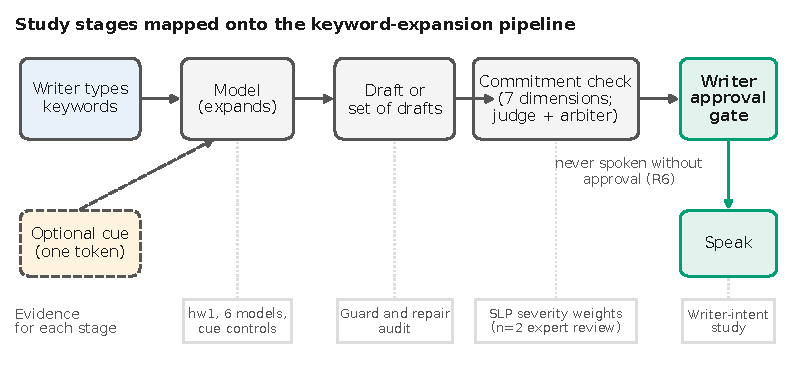
\includegraphics[width=\linewidth]{figs/fig1_pipeline.pdf}
\caption{Keyword-expansion pipeline with the approval gate, and where each study of this paper plugs in. A one-token cue is optional; nothing is spoken until the writer approves a draft (requirement R6, from the design consultants who use AAC). Schematic; no data.}\label{fig:pipeline}
\Description{Keyword-expansion pipeline with the approval gate, and where each study of this paper plugs in.}
\end{figure}

\subsection{Items, channels, models}\label{sec:m-items}

\paragraph{Families and dimensions.}
A \emph{family} is a minimal pair of source sentences that share their content words and differ on one \emph{critical} dimension: polarity, agent (who acts), certainty, speech act (statement, question or request), politeness, or time/quantity.
The two members of a pair, variants A and B, are rendered from the same keywords, so the keywords alone cannot tell them apart.
The extractor answers the family's critical question for every output and five general questions (polarity, speech act, agent, certainty, politeness), and it answers an added-content question.
These are the seven fields that the human checks below validate.

\paragraph{Channels.}
Each variant is shown to the model through five \emph{channels} that differ in how much of the message the person supplied.
\emph{Bare} gives the keywords only.
\emph{Non-critical} adds one content word that does not bear on the critical dimension and so matches the length of a cue.
\emph{Chip} adds the critical value as a one-token cue such as \texttt{[NOT]}, \texttt{[?]} or \texttt{[PLAIN]}.
\emph{All-chips} adds every cue the variant needs.
\emph{Full} gives the source sentence itself.
The chip is a probe of whether supplied information is used, not a proposed interface: its real cost depends on the access method, and a plain-word cue and an irrelevant-chip control are scored as separate channels (Section~\ref{sec:default}).
Table~\ref{tab:worked} shows one family through all five channels.

\paragraph{Evidence sets.}
The primary set is the human-written pairs (\emph{hw1}).
\jmhwWritersKept{} adult non-author classmates wrote \jmhwCand{} candidate minimal pairs and the keywords for them; three independent blind checkers per pair, who never saw model outputs, and a tie-break by one of six fixed checkers kept \jmhwKept{}, of which \jmhwFamilies{} are analysed after the exclusions stated in the hw1 report.
Each contrast rests on \jmhwWrMin{} to \jmhwWrMax{} writers.
Generation ran on all candidates before the checks, so dropped pairs are removed at analysis time.
A confirmation set of machine-written families with three pre-specified contrasts, and a development set used to build the prompts and codebook, are reported in the concurrent papers and enter here only where cited.

\paragraph{Models and prompt.}
Six models from \jmbreadthFamilies{} families write one sentence per request: Qwen2.5-7B-Instruct, Llama-3.1-8B-Instruct, Gemma-3-4B-it, Qwen2.5-14B-Instruct and Mistral-Nemo-12B-Instruct (4-bit GGUF, llama.cpp, local) and one API model, gpt-6.1-terra.
All use one fixed one-sentence prompt (\texttt{P0}) with greedy decoding; the prompt includes a short legend of the cues, and the no-legend arms of Section~\ref{sec:default} test whether the legend matters.
The hw1 run comprises \jmhwRequests{} requests.
A lite commercial Gemini model was added later under the same prompts as a seventh, machine-API replication, and is labelled as such where its rows appear.
Reissuing the same request reproduces the text for \jmndLocalMin{} to \jmndLocalMax{}\% of local requests and \jmndApiMin{} to \jmndApiMax{}\% of API requests, so every comparison is made on stored outputs for the same request and not on fresh draws.

\begin{table}[t]
\caption{One hw1 polarity family through the five channels, with the verdict each channel can give. Selection rule, declared before the draw: polarity families ordered by SHA-256 of the family id; the first family in which the bare output commits to the wrong value while the chip output matches; models in alphabetical order, then variant A, then B (here \jmexPolQual{} qualifying families; model \texttt{gemma3-4b}, variant B, target \emph{negated}; stored outputs and stored labels, not edited). Source sentence: ``The supervisor does not read my schedule.'' Rate the example represents: a committed bare output has the wrong value for the variant in \jmexPolWrong{}\% [\jmexPolWrongLo{}, \jmexPolWrongHi{}] of \jmexPolBareN{} bare rows (\jmexPolWriters{} writers), the design ceiling of a pair that shares one bare input, not a finding about models; given the chip, the output matches the target in \jmexPolChip{}\% [\jmexPolChipLo{}, \jmexPolChipHi{}] of \jmexPolChipN{} rows.}
\label{tab:worked}
\small
\setlength{\tabcolsep}{3pt}
\begin{tabular}{@{}l p{3.15cm} p{2.5cm} l l@{}}
\toprule
Channel & Input shown & Stored output & Label & Verdict\\
\midrule
Bare & \texttt{supervisor read} & The supervisor read. & affirmative & assumption (wrong value)\\
Non-critical & \texttt{supervisor read schedule} & The supervisor read the schedule. & affirmative & assumption (wrong value)\\
Chip & \texttt{[NOT] supervisor read} & The supervisor did not read. & negated & kept\\
All-chips & \texttt{[NOT] [TELL] [THEY] supervisor read} & The supervisor did not read. & negated & kept\\
Full & typed source sentence & The supervisor does not read my schedule. & negated & kept\\
\bottomrule
\end{tabular}
\end{table}

\subsection{Attribution by construction}\label{sec:m-attr}

Attribution is a property of the design, not a judgment about each output.
Let $C(x)$ be the set of dimensions whose value input $x$ fixes: the chip or the typed sentence fixes the critical dimension in the chip, all-chips and full channels, and nothing fixes it in the bare and non-critical channels.
For an output $y$ with extracted value $L_d(y)$ on dimension $d$ and meant value $s_d$:
\begin{itemize}
\item \textbf{Violation.} $d\in C(x)$ and $L_d(y)$ is not admissible for $s_d$. The model held the value and did not keep it. This is the only miss a checker can enforce.
\item \textbf{Assumption.} $d\notin C(x)$ and $L_d(y)$ is a committed value. The model chose a reading the input left open. An assumption is not a pass or a fail; we report its direction and share.
\item \textbf{Loss.} $d\notin C(x)$ and $L_d(y)\neq s_d$. The writer's value never reached the model. Loss and assumption are the same open-channel event seen from the interface (the value was lost) and from the model (it committed anyway); a loss is never charged as a violation.
\end{itemize}
Because the two variants of a pair share their open-channel input, a model that commits is wrong on exactly one of them, so paired match in an open channel has a ceiling that the design fixes; the quantity of interest is the gap between open and cue channels, not the open-channel rate.
The cue gain (chip minus non-critical) measures how much of the loss a cue recovers, and the irrelevant-chip control separates cue content from added tokens (Section~\ref{sec:default}).
A reference-fidelity score would charge the model for what the interface omitted; this rule does not.

Verdicts are computed in code from labels, the item specification and the channel, identically for treated and untreated outputs.
Plain assertion is honoured by emphatic certainty; unresolved critical labels are excluded and counted, not filled from either extractor prompt; and the added-content field is carried as a descriptive rate and enters no verdict rule.
Refusal and acceptance speech-act families are quarantined from every primary estimate because their predicate failed the oracle tests of Section~\ref{sec:m-oracle}.
The rule decides only whether explicit, text-level values are kept.
It does not judge fluency, reference resolution or whether the writer would accept the sentence; the writer-grounded analysis of Section~\ref{sec:waterfall} extends the attribution to that question.

\paragraph{Input honesty (R5).}
A failure cannot be charged to a model if the displayed input misstated the claim.
A validator therefore decodes the rendered input and rejects any cue that contradicts the source before generation.
Replayed on \jmtNineInputs{} chip inputs from the confirmation, composition and hw1 sets, it found \jmtNineConflicts{} conflicts; \jmtNineCompat{} inputs were verified compatible and \jmtNineUnknown{} (time chips and one long alias) lie outside its decoder, with \jmtNineGenCalls{} generation or judge calls.
Two defects found while building the harness, a relaxed acceptance predicate and an input-builder fallback, and the regression test each produced, are traced in the concurrent archival paper~\cite{concurrent_se4all}.

\subsection{Extractor, judge pair and arbiter}\label{sec:m-judge}

The extractor is gpt-6.1-sol at low reasoning effort, a model that is not among those under test.
It sees the output alone, not the source, the model or the channel, except for the added-content question, which also sees the visible input.
Two prompt variants, J1 and J2, differ in wording and option order.
On hw1 they labelled \jmhwUnits{} unique output units and agreed on the critical label for \jmhwJJCrit{}\% ($\kappa=\jmhwJJCritKappa{}$); the remaining \jmhwNeedArb{} units (\jmhwNeedArbShare{}\%) went to a blind arbiter.
The arbiter is a Claude model from a different family than the judge (claude-opus-5-5 for the confirmation set, claude-sonnet-5-5 for the other runs) and sees only the output text, the critical question and its options.
No J1 fallback enters a primary estimate, and every hw1 critical label is resolved by agreement or by the arbiter.
In the confirmation set the arbiter resolved \jmwcArbUnits{} units (\jmwcArbRows{} rows) after outcomes were known, blind to reference, model and condition, and the unknown-masked analysis is kept as a sensitivity analysis.
One tested model, gpt-6.1-terra, shares a vendor with the judge; its critical-label $\kappa$ against humans is reported with the other models in Section~\ref{sec:m-gates}.

\subsection{Testing the checker}\label{sec:m-oracle}

The checker is the extractor plus the verdict code; we test it as software, in the spirit of the test-oracle and mutation-analysis literature~\cite{weyuker1982nontestable,barr2015oracle,jia2011mutation}: an authorized change must pass and an unauthorized one must fail.
Table~\ref{tab:oracle} lists the evidence in the order of how far it is from our own hands.

\begin{table}[t]
\caption{Checker evidence. Authored rows use sentences we wrote or edited; the real-output rows seed one-value edits into stored hw1 outputs (seed \jmorrSeed{}; four booster mutants, which the contract tolerates, are excluded from the mutant counts); the last rows compare the judge's verdicts with the consensus of human coders on unedited outputs from held-out sets (Parts 10 and 13). Intervals are Wilson 95\%. None of the first two groups is an error rate on unedited outputs.}
\label{tab:oracle}
\small
\setlength{\tabcolsep}{3pt}
\begin{tabular}{@{}p{5.6cm} r@{}}
\toprule
Check & Result\\
\midrule
\multicolumn{2}{@{}l}{\emph{Authored inputs}}\\
Identity: unchanged source passes; false alarms & \jmorIdFaK{}/\jmorIdFaN{}\\
Scoped one-value mutants detected & \jmorMutK{}/\jmorMutN{}\\
Keyed challenge, mutants detected, production rule & \jmorKeyMutK{}/\jmorKeyMutN{}\\
\quad acceptance group only & \jmorKeyAccProdK{}/\jmorKeyAccProdN{}\\
\quad strict rule, no acceptance relaxation & \jmorKeyMutStrictK{}/\jmorKeyMutStrictN{}\\
Keyed challenge controls, false alarms & \jmorKeyCtlK{}/\jmorKeyCtlN{}\\
\midrule
\multicolumn{2}{@{}l}{\emph{Seeded edits of real outputs} (mutants caught; false alarms on \jmorrJFaN{} controls)}\\
Judge (J1, J2, arbiter) & \jmorrJMutK{}/\jmorrJMutN{} [\jmorrJMutLo{}, \jmorrJMutHi{}]\%; \jmorrJFaK{}/\jmorrJFaN{}\\
Surface lexicon (near-circular) & \jmorrSMutK{}/\jmorrSMutN{}; \jmorrSFaK{}/\jmorrSFaN{}\\
String overlap & \jmorrOMutK{}/\jmorrOMutN{}; \jmorrOFaK{}/\jmorrOFaN{}\\
\midrule
\multicolumn{2}{@{}l}{\emph{Unedited outputs, held-out human consensus} (precision; recall, \%)}\\
Violation verdict (\jmnatHoViolPos{} positives) & \jmnatHoViolP{} [\jmnatHoViolPLo{}, \jmnatHoViolPHi{}]; \jmnatHoViolR{} [\jmnatHoViolRLo{}, \jmnatHoViolRHi{}]\\
Preservation-failure verdict (\jmnatHoPresPos{} positives) & \jmnatHoPresP{} [\jmnatHoPresPLo{}, \jmnatHoPresPHi{}]; \jmnatHoPresR{} [\jmnatHoPresRLo{}, \jmnatHoPresRHi{}]\\
\bottomrule
\end{tabular}
\end{table}

\paragraph{Authored faults.}
An unchanged source injected as its own output must pass (the identity test), and a hand-written one-value change must be caught (scoped mutants).
A keyed challenge set of controls and one-feature mutants, with keys hashed before the first extractor call, has four groups: acceptance, embedded actors, question versus request, and mitigated requests.
The production rule detects \jmorKeyMutK{} of \jmorKeyMutN{} keyed mutants; the strict rule without the acceptance relaxation detects \jmorKeyMutStrictK{} of \jmorKeyMutStrictN{}, and the relaxation accounts for the difference, using up the pre-specified miss tolerance.
This is why refusal and acceptance families are quarantined: removing a false alarm from the acceptance predicate removed fault sensitivity.

\paragraph{Faults in real outputs.}
Hand-written faults are easy.
We therefore seeded \jmorrNAll{} one-value mutants into stored hw1 outputs that the checker had scored as preserving, with operators for each dimension (negation insertion and removal, speech-act flips, agent swaps, hedge insertion and removal, politeness addition and removal, time shifts), and drew \jmorrJFaN{} meaning-preserving surface edits as controls.
The judge caught \jmorrJMutK{} of \jmorrJMutN{} mutants with \jmorrJFaK{} false alarms, and no unresolved rows.
A surface lexicon of negation, hedge, politeness, tense and question cues scored \jmorrSMutK{} of \jmorrSMutN{} with \jmorrSFaK{} false alarms, and string overlap \jmorrOMutK{} of \jmorrOMutN{} with \jmorrOFaK{} false alarms.
The lexicon matches the cues the operators insert, so its score shows that the operators are lexically shallow and not that a lexicon is an adequate checker; the judge's advantage shows mainly on controls.

\paragraph{Faults nobody seeded.}
Seeded faults are faults we thought of.
The test on unedited outputs uses the human-coded sets of Section~\ref{sec:m-gates}: on the two sets not used to build the codebook, the judge's violation verdicts have precision \jmnatHoViolP{}\% and recall \jmnatHoViolR{}\% against the human consensus (\jmnatHoViolPos{} positives in \jmnatHoUnitsViol{} verdicts), and its preservation-failure verdicts \jmnatHoPresP{}\% and \jmnatHoPresR{}\% (Table~\ref{tab:oracle}).
Each set has few positives, so the intervals are wide.
Machine agreement is not validation: on a keyed challenge sentence, ``I can't wait to go to the party,'' the judge and the machine panel read \emph{negated}, a known blind spot for idiomatic negation, which is why no claim here rests on machine-panel agreement.

\subsection{Validating the extractor against human coders}\label{sec:m-gates}

Four human gates compare the extractor's final label with the plurality label of trained human coders on stored outputs (Table~\ref{tab:gates}).
Coders labelled the same fields from the stored output with the same options as the judge, after being taught the same codebook with practice items.
The development gate (H7) used the extraction inventory from which the codebook was built.
round~10 coded fresh outputs from the confirmation, composition and guard-transfer runs; round~12 coded outputs for keywords that other annotators typed for stored messages; round~13 coded outputs for the human-written pairs.
Rounds~10, 12 and 13 are therefore later checks on outputs the harness was not developed on.
Each gate samples stored outputs by a seeded draw and keeps a seeded quarter for calibration; $\kappa$ is computed on the remaining test split.
The stored rule excludes ties and unsure answers from the reference; the strict rule counts them as disagreement, and the table reports the strict rule with a family-cluster bootstrap interval.

\begin{table}[t]
\caption{Extractor against human coders, test split (Cohen's $\kappa$). Strict rule: ties and unsure answers count as disagreement; intervals are family-cluster bootstrap 95\%. Human--human and judge--human $\kappa$ are computed on the same items for the critical field. All coders were adult non-author classmates. Added content is the weakest field in Parts 10 and 13.}
\label{tab:gates}
\footnotesize
\setlength{\tabcolsep}{2.5pt}
\begin{tabular}{@{}l r r r l r r r r@{}}
\toprule
Gate & Coders & Items (test) & Stored $\kappa$ & Strict critical $\kappa$ [CI] & Hum--hum & Judge--hum & Speech act & Added\\
\midrule
H7 (development) & \jmhgHSevenCoders{} & \jmhgHSevenSampled{} (\jmhgHSevenTest{}) & \jmhgHSevenCritRZero{} & \jmhgHSevenCrit{} [\jmhgHSevenCritLo{}, \jmhgHSevenCritHi{}] & \jmhgHSevenHH{} & \jmhgHSevenJH{} & \jmhgHSevenAct{} & \jmhgHSevenAdded{}\\
Round 10 (fresh runs) & \jmhgPTenCoders{} & \jmhgPTenSampled{} (\jmhgPTenTest{}) & \jmhgPTenCritRZero{} & \jmhgPTenCrit{} [\jmhgPTenCritLo{}, \jmhgPTenCritHi{}] & \jmhgPTenHH{} & \jmhgPTenJH{} & \jmhgPTenAct{} & \jmhgPTenAdded{}\\
Round 12 (typed keywords) & \jmhgPTwelveCoders{} & \jmhgPTwelveSampled{} (\jmhgPTwelveTest{}) & \jmhgPTwelveCritRZero{} & \jmhgPTwelveCrit{} [\jmhgPTwelveCritLo{}, \jmhgPTwelveCritHi{}] & \jmhgPTwelveHH{} & \jmhgPTwelveJH{} & \jmhgPTwelveAct{} & \jmhgPTwelveAdded{}\\
Round 13 (human-written pairs) & \jmhgPThirteenCoders{} & \jmhgPThirteenSampled{} (\jmhgPThirteenTest{}) & \jmhgPThirteenCritRZero{} & \jmhgPThirteenCrit{} [\jmhgPThirteenCritLo{}, \jmhgPThirteenCritHi{}] & \jmhgPThirteenHH{} & \jmhgPThirteenJH{} & \jmhgPThirteenAct{} & \jmhgPThirteenAdded{}\\
\bottomrule
\end{tabular}
\end{table}

On the critical field the extractor's strict-rule $\kappa$ is at least \jmhgCritMin{} in every gate, with the lowest lower interval bound at \jmhgCritLoMin{}, against a pre-specified gate of \jmhgGate{}.
In every gate the judge--human $\kappa$ sits just below the human--human $\kappa$ on the same items, so the extractor is close to, not above, the agreement that two people reach.
By model, the critical-field $\kappa$ on the development gate lies between \jmhgHSevenModelMin{} and \jmhgHSevenTerra{} (gpt-6.1-terra, $n=\jmhgHSevenTerraN{}$).
The added-content field is the exception: its $\kappa$ is \jmhgPTenAdded{} on round~10 and \jmhgPThirteenAdded{} on round~13 (J1--J2 agreement on hw1 is $\kappa=\jmhwJJAddedKappa{}$), so no verdict or estimate here is built on it.
These gates cover untreated outputs and the codebook is shared between humans and judge; they validate extraction of explicit markers, not repaired or rewritten text, which the audits of Section~\ref{sec:m-instruments} address.

\subsection{Validating the arbiter against human coders (arbiter check)}\label{sec:m-arbiter}

The arbiter decides every unit on which the two extractor prompts disagree, so it carries the hardest labels.
The arbiter check asks people to code exactly those units.
Each of \jmpOneNinePeople{} annotators coded a seeded set of items, two coders per item.
The key holds \jmpOneNineArbItems{} arbiter units, stratified by run and by the precedent the arbiter applied (for example, ``I want X, please'' is a request), on every one of which J1 and J2 disagreed, and \jmpOneNineCanYouItems{} ``Can you\ldots?'' or ``Could you\ldots?'' outputs for which the codebook example was hidden.
Coders did not receive items from their own pairs or keyword sets.
Of the \jmpOneNineArbExpected{} codings on arbiter units, \jmpOneNineArbLabelledN{} carried a label; the remaining \jmpOneNineArbUnlabelledShare{}\% were unsure or blank and are excluded, not counted as disagreement, so the agreement below is conditional on a person committing to a label.
Intervals are Wilson and descriptive, because codings are not independent.

\begin{table}[t]
\caption{Humans against the arbiter and each judge prompt on the \jmpOneNineArbItems{} arbiter units (\jmpOneNineCodings{} labelled codings, all units ones on which J1 and J2 disagreed). The arbiter sided with J1 on \jmpOneNineSidedJOne{} units, with J2 on \jmpOneNineSidedJTwo{} and with neither on \jmpOneNineSidedNeither{}.}
\label{tab:arbiter}
\small
\begin{tabular}{@{}l r r@{}}
\toprule
Reference & Agreement with humans (\%) [95\% CI] & Cohen's $\kappa$\\
\midrule
Arbiter & \jmpOneNineAgreeArb{} [\jmpOneNineAgreeArbLo{}, \jmpOneNineAgreeArbHi{}] & \jmpOneNineKappaArb{}\\
J1 & \jmpOneNineAgreeJOne{} [\jmpOneNineAgreeJOneLo{}, \jmpOneNineAgreeJOneHi{}] & \jmpOneNineKappaJOne{}\\
J2 & \jmpOneNineAgreeJTwo{} [\jmpOneNineAgreeJTwoLo{}, \jmpOneNineAgreeJTwoHi{}] & \jmpOneNineKappaJTwo{}\\
\bottomrule
\end{tabular}
\end{table}

Humans side with the arbiter more often than with either prompt (Table~\ref{tab:arbiter}).
They match the arbiter on \jmpOneNineMatchJOneSide{}\% [\jmpOneNineMatchJOneSideLo{}, \jmpOneNineMatchJOneSideHi{}] of codings where it sided with J1 and \jmpOneNineMatchJTwoSide{}\% [\jmpOneNineMatchJTwoSideLo{}, \jmpOneNineMatchJTwoSideHi{}] where it sided with J2, so the arbiter is not simply the more frequent prompt.
Where both coders of an item gave a label, they agree with each other on \jmpOneNineHHAgree{}\% (\jmpOneNineHHItems{} items, $\kappa=\jmpOneNineHHKappa{}$); \jmpOneNineSplit{} arbiter items split their coders.
The disagreements with the arbiter concentrate in a few precedent tags with few items each (for example, ``I want X, please'' and ``I tell you to\ldots''); the supplement lists them with their counts, and we do not pool them away.
On the codebook rule that ``Can you\ldots?'' is a request, \jmpOneNineCanYouRequest{}\% [\jmpOneNineCanYouRequestLo{}, \jmpOneNineCanYouRequestHi{}] of \jmpOneNineCanYouLabelled{} labelled codings chose request or command, from coders who had not been shown the rule; the alternative coding as a question is not what people do.
\paragraph{What the exclusion and the dependence do to the estimate.}
Excluding unsure or blank codings matters: if every one of the \jmpOneNineSensUnsure{}\% unlabelled codings on the arbiter units (\jmpOneNineSensLabelled{} labelled of \jmpOneNineSensTotal{}) were counted as a disagreement, agreement with the arbiter would be \jmpOneNineSensLowerBound{}\%, so the \jmpOneNineAgreeArb{}\% is an agreement among codings where a person committed, and these are the units on which two prompts already disagreed.
Codings share items and coders, so we resampled items as clusters: the interval is \jmpOneNineSensBootLo{} to \jmpOneNineSensBootHi{}\%, close to the descriptive Wilson interval.
Dropping any one coder moves agreement only between \jmpOneNineSensLooMin{}\% and \jmpOneNineSensLooMax{}\%.
Per-coder agreement is far noisier (\jmpOneNineSensCoderMin{} to \jmpOneNineSensCoderMax{}\% over the \jmpOneNineSensCoderN{} coders with at least five labelled codings), and the \jmpOneNineSensCoderPairs{} coder pairs share only a few items each, so a kappa per coder pair is not estimable; the only pair-level statistic we report is the human--human agreement on items where both coders labelled.
We therefore call the arbiter \emph{checked against human codings of the disputed units}, and do not call it validated in general: the evidence is a moderate-sized check of the hardest units, with a stated attrition.

The consequence for the method is fixed in advance of every analysis: arbiter labels are the reference for disputed units, no J1 fallback enters a primary estimate, and the effect of recoding ``Can you\ldots?'' is reported next to the primary estimate (Section~\ref{sec:default}).

\subsection{Writer-grounded and expert instruments}\label{sec:m-instruments}

Four further instruments supply the human evidence of later sections; their results are not repeated here.
\textbf{Repair-usability audit (blind three-rater audit).}
\jmpOneSevenItemsPerArm{} repaired texts and \jmpOneSevenItemsPerArm{} controls, plus a secondary arm of the pre-repair originals, were rated blind to arm by \jmpOneSevenRaters{} raters, \jmpOneSevenPerItem{} per item.
The primary endpoint, the item-level consensus ``usable'' (strict majority of its raters), and the decision rule for repaired minus control were frozen in the repository before any rating was returned; the rule and its three outcomes are stated in the protocol and applied unchanged.
\textbf{Writer-intent check (the writer-intent study).}
Each of the \jmpOneEightWriters{} writers rated \jmpOneEightPerWriter{} outputs for their own pairs, half from the bare channel and half from the chip channel, choosing which variant the sentence says (A, B, something else, unclear) and whether they would accept it as their message.
The judge labels the critical dimension only, while the writer judges the whole message; the instrument is writer-intent agreement and not validation by AAC users.
\textbf{Expert annotators.}
Two anonymous speech-language pathologists rated the seriousness of each kind of silent meaning change on an anchored scale and rated stored outputs blind to arm; the result is an expert review by two raters, not a population estimate.
\textbf{Design consultants.}
Two paid design consultants who use AAC reviewed the requirements and example outputs; every suggestion and the resulting change or non-change is logged, and we report requirement changes, not the consultants' experiences.
Annotators were adult non-author university classmates who consented and were paid (payment and food); the two expert annotators and two consultants were paid under written agreements.
No institutional review determination was sought.

\subsection{Estimation}\label{sec:m-est}

Contrasts are differences of row-weighted means over targets, where a target is one (item, model, channel, variant) outcome and the model roster is fixed.
Intervals are pointwise 95\% percentile intervals from \jmhwBootN{} cluster resamples (seed \jmhwSeed{}): writers are the clusters for hw1 and construction clusters for the confirmation set.
Proportions of codings use Wilson intervals, and $\kappa$ intervals use family-cluster bootstrap.
With \jmhwWrMin{} to \jmhwWrMax{} writers per contrast, the writer-cluster intervals are optimistic, and we claim direction and consistency across writers, not interval width.
No interval corrects for exploratory selection or for extractor error beyond the validation above.
Analyses were pre-specified and git-timestamped; we do not call them pre-registered, and the public hash deposits post-date the confirmation freeze and do not certify it.
Numbers in tables and text are generated from the stored analysis files by a script, and the verdict rule can be re-run on stored labels with no model call.

% Section 3 (Studies and Results I) of the TACCESS manuscript.
% In main.tex replace the \section{Results I...} and \section{Results II...} stubs by % Section 3 (Studies and Results I) of the TACCESS manuscript.
% In main.tex replace the \section{Results I...} and \section{Results II...} stubs by % Section 3 (Studies and Results I) of the TACCESS manuscript.
% In main.tex replace the \section{Results I...} and \section{Results II...} stubs by \input{sections/s3}.
% Every number is a \jm... macro from make_macros.py (function s3() and earlier functions); no hand-typed numbers.
% Examples are stored outputs chosen by a declared rule (analysis/hw1/examples.md). Citations are limited to
% records already in refs.bib; nothing new was opened for this section.
% Labels defined here: sec:default (section), sec:basecost, sec:robust, sec:cue, sec:price, sec:asks, sec:guard, sec:usability, sec:severity.
% Needs \usepackage{booktabs} (acmart loads it).

\section{Studies and Results I: Defaults, Cue Restoration and the Guard}\label{sec:default}

This section reports the studies that establish what the default costs and what repairs it. Each study states its population, its estimator and its denominator, and each result is bounded once, where it is reported. We begin with the cost of the default measured against what people actually type (\S\ref{sec:basecost}), test whether the default belongs to the prompt or to the models (\S\ref{sec:robust}), show that a cue restores the commitment and that the cue's content is what does it (\S\ref{sec:cue}), price the restoration per 1,000 messages on the same items (\S\ref{sec:price}), ask whether any rule for when to ask beats chance (\S\ref{sec:asks}), and then evaluate the guard against a no-feedback baseline (\S\ref{sec:guard}), a blind human audit of its repairs (\S\ref{sec:usability}) and expert severity weights (\S\ref{sec:severity}).

\paragraph{Conventions common to all studies.}
Model outputs are labelled by two machine judges (J1, J2); disagreements on the critical commitment go to a blind arbiter that sees only the output text, and no label falls back to J1 when the arbiter is missing. Intervals are 95\% percentile bootstrap intervals clustered by writer (human-written pairs), by family (machine-written families and the guard) or by message (the elicitation sample). The human-written, legend, control and guard analyses use \jmconvBoot{} resamples with seed \jmconvSeed{}, the same-items study uses \jmconvBootFOne{} resamples with seed \jmconvSeedFOne{}, and the elicitation-sample prices and ask-policy contrasts use the resample counts stated in their reports. Rates ``per 1,000 messages'' are rates over the sampled units, not deployment rates. Where a decision rule governs a verdict (the legend test, the same-items comparisons, the guard baseline and the usability audit), it was written down and git-timestamped before the outcomes it governs were generated or returned; we do not call any of the studies pre-registered. Machine labels are used throughout this section; where a human check of the machine labels exists it is reported in the study that uses the labels, and the checks that have not yet returned are named as such.

% ------------------------------------------------------------------------------------------------
\subsection{What the Default Costs, Priced Against Human Base Rates}\label{sec:basecost}

\paragraph{Setting.}
A keyword string that omits a cue leaves the model to choose a reading, and the choice is a default. Whether a default is a good guess depends on how often the omitted cue was present in what the writer meant. We measured that base rate from people. The elicitation sample consists of \jmtTwoMessages{} source messages from an AAC-style corpus (\jmtTwoCorpus{} messages in total, of which \jmtTwoCorpusNeg{}\% are negated by a detector label), each shortened to keywords by three human keyword sets, giving \jmtTwoUnits{} keyword units. Stored outputs of \jmbreadthOrigModels{} generators were scored for three commitment dimensions (negation, politeness, sentence type), the dimensions for which a lexical test of ``the keywords carry the cue'' exists. The source cue labels are detector labels; these labels have no human check, so the prices below carry the detector's error and are provisional.

\paragraph{Affirmative is the right guess for negation; the cost is the asymmetry.}
Among keyword strings with no negation word, the source was negated in \jmtTwoPostPol{}\% [\jmtTwoPostPolLo{}, \jmtTwoPostPolHi{}] of cases (\jmtTwoPostBayesPol{}\% by Bayes' rule with the corpus prevalence; \jmtTwoPolRandHalf{}\% in the unweighted random half). Guessing the affirmative reading is therefore correct for all but a few messages in a hundred, and the models take it: they output an affirmative sentence for \jmtTwoAffGivenNoNeg{}\% of such inputs. The direction of the default is the rational one, which is consistent with prior reports that language models state negative content too positively \cite{chen2023say}; we do not present the default as new. What the base rate adds is the price. People dropped the negation word from \jmtTwoDroppedPol{}\% [\jmtTwoDroppedPolLo{}, \jmtTwoDroppedPolHi{}] of the negated messages, so an affirmative sentence silently reverses \jmtTwoRevPol{} [\jmtTwoRevPolLo{}, \jmtTwoRevPolHi{}] messages per 1,000, while a spurious negation is introduced in \jmtTwoSpurPol{} per 1,000. The affirmative guess breaks even with the opposite guess only if a reversed negation costs less than \jmtTwoBreakPol{} times a spurious one, and a prompt would have to be shown on about \jmtTwoQueriesPol{} inputs per reversal it prevents. The models' confidence also exceeds the evidence: they assert a negation on \jmtTwoModelCuePol{}\% of these inputs where the base rate is \jmtTwoPostPol{}\%.

\paragraph{Politeness and sentence type differ in kind.}
For politeness the default is calibrated: the source was polite in \jmtTwoPostPolite{}\% [\jmtTwoPostPoliteLo{}, \jmtTwoPostPoliteHi{}] of unmarked inputs and models add politeness to \jmtTwoModelCuePolite{}\%. Politeness the writer typed is lost for \jmtTwoRevPolite{} messages per 1,000, with a break-even ratio of \jmtTwoBreakPolite{}, so the asymmetry is milder than for negation; the opposite error, politeness added to a plain message, occurs in \jmtTwoSpurPolite{} per 1,000. For sentence type the statement default is not the Bayes-preferred guess at all: the source was a question, request or other non-statement in \jmtTwoPostAct{}\% [\jmtTwoPostActLo{}, \jmtTwoPostActHi{}] of unmarked inputs, while models assert one on only \jmtTwoModelCueAct{}\%, and \jmtTwoRevAct{} [\jmtTwoRevActLo{}, \jmtTwoRevActHi{}] messages per 1,000 have their sentence type reversed or flattened (break-even ratio \jmtTwoBreakAct{}: the statement default pays only if the two errors cost about the same).
Table~\ref{tab:basecost} collects these rows.

\begin{table}[t]
\caption{The default priced against human base rates (elicitation sample, \jmtTwoUnits{} keyword units from \jmtTwoMessages{} messages; Horvitz--Thompson weights; message-bootstrap 95\% intervals). Prior is the share of keyword strings without the cue whose source message carried it; model asserts cue is the share of such inputs for which the model's output asserts the cue-bearing value. Reversals are messages whose source has the cue, whose keywords lack it and whose output lacks it; the opposite error is an output that asserts the cue when the source lacks it; break-even is the cost ratio of a reversal to an opposite error at which the default stops paying. Source labels are detector labels.}\label{tab:basecost}
\footnotesize
\begin{tabular}{@{}lccccc@{}}
\toprule
Dimension & Prior [95\% CI] & Model asserts cue & Reversals /1,000 [CI] & Opposite /1,000 & Break-even \\
\midrule
Negation (affirmative default) & \jmtTwoPostPol{}\% [\jmtTwoPostPolLo{}, \jmtTwoPostPolHi{}] & \jmtTwoModelCuePol{}\% & \jmtTwoRevPol{} [\jmtTwoRevPolLo{}, \jmtTwoRevPolHi{}] & \jmtTwoSpurPol{} & \jmtTwoBreakPol{} \\
Politeness (plain default) & \jmtTwoPostPolite{}\% [\jmtTwoPostPoliteLo{}, \jmtTwoPostPoliteHi{}] & \jmtTwoModelCuePolite{}\% & \jmtTwoRevPolite{} [\jmtTwoRevPoliteLo{}, \jmtTwoRevPoliteHi{}] & \jmtTwoSpurPolite{} & \jmtTwoBreakPolite{} \\
Sentence type (statement default) & \jmtTwoPostAct{}\% [\jmtTwoPostActLo{}, \jmtTwoPostActHi{}] & \jmtTwoModelCueAct{}\% & \jmtTwoRevAct{} [\jmtTwoRevActLo{}, \jmtTwoRevActHi{}] & \jmtTwoSpurAct{} & \jmtTwoBreakAct{} \\
\bottomrule
\end{tabular}
\end{table}

\paragraph{The same default in human-written pairs.}
The human-written pairs (\S\ref{sec:cue}) test the default where the truth is known. Each pair differs in one commitment and shares one bare input, so a model that commits to one reading is wrong on exactly one variant and the true affirmative rate is 50\%. On the bare channel the models chose the affirmative reading in \jmtTwoHwAffShare{}\% of valid outputs.

\paragraph{Bound.}
Source cue labels are detector labels, the sentence-type ``no cue'' condition is a lexical proxy, the frame prevalence of negation (\jmtTwoPrevPol{}\%) exceeds the corpus value, and the prices are rates over a sampled elicitation frame. We therefore read the table as the cost structure of the default, not as a deployment rate.

% ------------------------------------------------------------------------------------------------
\paragraph{Appendix material.} The model-breadth tables and legend test (Appendix~\ref{sec:robust}) and the ask-policy arithmetic (Appendix~\ref{sec:asks}) are in the appendix; the main text uses only their headline results.

\subsection{A Cue Restores the Commitment, and the Content of the Cue Does It}\label{sec:cue}

\paragraph{Human-written pairs.}
To move beyond machine-written test items, \jmhwWritersTotal{} adult non-author classmates wrote sentence pairs that differ in one commitment and chose their own keywords; pairs were kept only after classmate checks, and \jmhwFamilies{} families were analysed, with \jmhwChipGainWriters{} to \jmhwAffShareWriters{} writers contributing to each contrast. Each family was expanded by \jmbreadthOrigModels{} models under bare keywords, a non-critical extra keyword, the cue as a one-token chip (for example \texttt{[NOT]}), the full cue set, and the full original text. The primary contrasts are those of the machine-written confirmation set (Holm-corrected over three); the human-written pairs are an exploratory replication of them. The chip gain over a non-critical word on speech act is \jmhwChipGain{} points [\jmhwChipGainLo{}, \jmhwChipGainHi{}] (\jmhwChipGainWriters{} writers, \jmhwChipGainFamilies{} families). When the full sentence is given, politeness is added to plain messages more often than it is removed from polite ones, by \jmhwPolGain{} points [\jmhwPolGainLo{}, \jmhwPolGainHi{}]. The bare affirmative share (\jmhwAffAll{}\%, \S\ref{sec:basecost}) is the third contrast. All three agree in direction and in decision with the machine-written confirmation set. Because each contrast rests on a handful of writers, we claim the direction and its consistency across writers and models, not the width of the intervals.

\paragraph{One stored case, by declared rule.}
The rule: order the analysed polarity families by the SHA-256 of the family identifier and take the first one in which a bare output commits to the wrong value while the chip output matches. That family is \texttt{hw-pol-075}, the model is Gemma-3-4B, and the target is the negated reading of ``The supervisor does not read my schedule.''

\begin{center}\small
\begin{tabular}{lll}
\toprule
Channel & Input & Stored output \\
\midrule
bare & \texttt{supervisor read} & ``The supervisor read.'' (affirmative) \\
chip & \texttt{[NOT] supervisor read} & ``The supervisor did not read.'' (negated) \\
\bottomrule
\end{tabular}
\end{center}

\noindent
In this dimension a bare output commits to the wrong value in \jmexPolBareWrong{}\% [\jmexPolBareWrongLo{}, \jmexPolBareWrongHi{}] of bare rows (the design ceiling), and when it does the chip output matches the target in \jmexPolRepair{}\% [\jmexPolRepairLo{}, \jmexPolRepairHi{}] of \jmexPolRepairN{} such rows. The same rule applied to speech act selects a family whose chip outputs match the target in a smaller share, \jmexActRepair{}\% [\jmexActRepairLo{}, \jmexActRepairHi{}] of \jmexActRepairN{} rows, in line with the larger residual for sentence type in \S\ref{sec:price}.

\paragraph{Six dimensions.}
Table~\ref{tab:sixdim} reports the cue gain for every measured dimension with its two controls. An irrelevant chip (a cue from another dimension, with the same token cost) adds about nothing on polarity, politeness, agent and time (at most \jmctlIrrelAddTime{} points) and a small amount on certainty (\jmctlIrrelAddCert{} [\jmctlIrrelAddCertLo{}, \jmctlIrrelAddCertHi{}]) and speech act (\jmctlIrrelAddAct{} [\jmctlIrrelAddActLo{}, \jmctlIrrelAddActHi{}]). The relevant chip beats the irrelevant chip by \jmctlOverIrrelAct{} to \jmctlOverIrrelTime{} points, so the gain is the content of the cue and not the presence of an extra token. A plain-language word delivers the same restoration as the chip within 5 points on every dimension except speech act; on speech act the word is better than the chip (chip minus word \jmctlOverWordAct{} points [\jmctlOverWordActLo{}, \jmctlOverWordActHi{}]). We do not claim that the chip is better than a plain word.

\begin{table}[t]
\caption{Cue restoration and its controls in human-written pairs (critical-commitment match, pooled over four models, writer-cluster 95\% intervals; points). Chip gain is chip minus non-critical word. Polarity and politeness bare matches sit at 50\% by design because both variants share one bare input; their informative quantity is the gain. Full input is the whole original sentence.}\label{tab:sixdim}
\small
\begin{tabular}{lccccc}
\toprule
Dimension & Bare match (\%) & Chip match (\%) & Chip gain [CI] & Irrelevant chip adds [CI] & Chip $-$ word [CI] \\
\midrule
Agent & \jmhwMatchBareAgent{} & \jmhwMatchChipAgent{} & \jmctlGAgent{} [\jmctlGAgentLo{}, \jmctlGAgentHi{}] & \jmctlIrrelAddAgent{} [\jmctlIrrelAddAgentLo{}, \jmctlIrrelAddAgentHi{}] & \jmctlOverWordAgent{} [\jmctlOverWordAgentLo{}, \jmctlOverWordAgentHi{}] \\
Time / quantity & \jmhwMatchBareTime{} & \jmhwMatchChipTime{} & \jmctlGTime{} [\jmctlGTimeLo{}, \jmctlGTimeHi{}] & \jmctlIrrelAddTime{} [\jmctlIrrelAddTimeLo{}, \jmctlIrrelAddTimeHi{}] & \jmctlOverWordTime{} [\jmctlOverWordTimeLo{}, \jmctlOverWordTimeHi{}] \\
Certainty & \jmhwMatchBareCert{} & \jmhwMatchChipCert{} & \jmctlGCert{} [\jmctlGCertLo{}, \jmctlGCertHi{}] & \jmctlIrrelAddCert{} [\jmctlIrrelAddCertLo{}, \jmctlIrrelAddCertHi{}] & \jmctlOverWordCert{} [\jmctlOverWordCertLo{}, \jmctlOverWordCertHi{}] \\
Polarity & \jmhwMatchBarePol{} & \jmhwMatchChipPol{} & \jmctlGPol{} [\jmctlGPolLo{}, \jmctlGPolHi{}] & \jmctlIrrelAddPol{} [\jmctlIrrelAddPolLo{}, \jmctlIrrelAddPolHi{}] & \jmctlOverWordPol{} [\jmctlOverWordPolLo{}, \jmctlOverWordPolHi{}] \\
Politeness & \jmhwMatchBarePolite{} & \jmhwMatchChipPolite{} & \jmctlGPolite{} [\jmctlGPoliteLo{}, \jmctlGPoliteHi{}] & \jmctlIrrelAddPolite{} [\jmctlIrrelAddPoliteLo{}, \jmctlIrrelAddPoliteHi{}] & \jmctlOverWordPolite{} [\jmctlOverWordPoliteLo{}, \jmctlOverWordPoliteHi{}] \\
Speech act & \jmhwMatchBareAct{} & \jmhwMatchChipAct{} & \jmctlGAct{} [\jmctlGActLo{}, \jmctlGActHi{}] & \jmctlIrrelAddAct{} [\jmctlIrrelAddActLo{}, \jmctlIrrelAddActHi{}] & \jmctlOverWordAct{} [\jmctlOverWordActLo{}, \jmctlOverWordActHi{}] \\
\bottomrule
\end{tabular}
\end{table}

\paragraph{Bound.}
\jmhwChipGainWriters{} to \jmhwAffShareWriters{} writers per dimension, one prompt template, and machine labels (with a blind arbiter for disputes); treated outputs have no separate human check beyond the arbiter check (Section~\ref{sec:m-arbiter}).

% ------------------------------------------------------------------------------------------------

\begin{figure}[t]
\centering
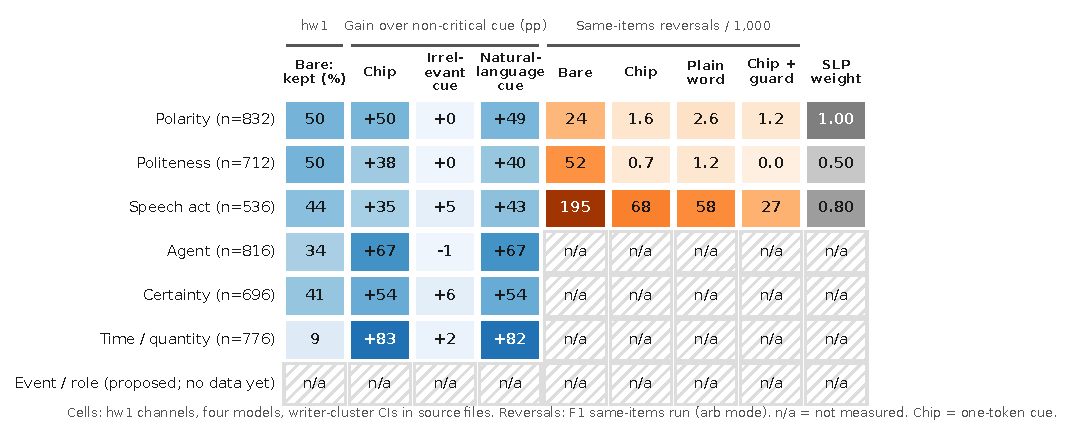
\includegraphics[width=\linewidth]{figs/fig4_dimension_table.pdf}
\caption{Dimension by intervention table. Left: share of bare outputs that keep the critical commitment (hw1, four models), and gain in that share over a non-critical cue for the chip, an irrelevant control cue and a natural-language cue. Right: same-items reversals per 1,000 messages for bare, chip, plain word and chip plus guard (\jmfOneUnits{} units; measured only for polarity, politeness and speech act), and the SLP severity weight (mean of two expert raters, $n=2$). Event/role structure is proposed but has no data. Every cell is printed; shading is redundant. Sources: \texttt{figs/figure\_values.json}.}\label{fig:table}
\Description{Dimension by intervention table.}
\end{figure}

\subsection{Cue Restoration Priced Per 1,000 Messages on the Same Items}\label{sec:price}

\paragraph{Design.}
The gains above come from constructed pairs. To price the cue on the messages that people actually shorten, we returned to the elicitation sample and took the \jmfOneUnits{} units whose source carried a cue that the human keywords dropped (polarity \jmfOneUnitsPol{}, politeness \jmfOneUnitsPolite{}, sentence type \jmfOneUnitsAct{}, the last a seeded subsample of question and request units). Each unit was regenerated by \jmfOneModels{} models (GPT-6.1-terra, Qwen2.5-7B, Llama-3.1-8B) under four arms at temperature zero: the stored bare output, the cue as a chip, the cue as a plain word, and the chip with the guard of \S\ref{sec:guard} monitoring the supplied chip. The restoration share is the proportion of units whose output honours the dropped cue; reversals per 1,000 messages are the exposure per 1,000 messages times one minus the restoration share. The bare arm reproduces the always-commit rates of \S\ref{sec:basecost}, so the unit construction matches. Disputed critical labels (\jmfOneArbRows{} rows) were resolved by the blind arbiter.

\paragraph{Results.}
Table~\ref{tab:price} gives the prices. Giving the cue on every message lowers polarity reversals from \jmfOneRevPolBare{} to \jmfOneRevPolChip{} (chip) or \jmfOneRevPolWord{} (word) per 1,000, and politeness reversals from \jmfOneRevPoliteBare{} to \jmfOneRevPoliteChip{} or \jmfOneRevPoliteWord{}. Chip and word are equivalent within 5 points on politeness (chip minus word \jmfOneChipMinusWordPolite{} points [\jmfOneChipMinusWordPoliteLo{}, \jmfOneChipMinusWordPoliteHi{}]) and not distinguishable on polarity (\jmfOneChipMinusWordPol{} [\jmfOneChipMinusWordPolLo{}, \jmfOneChipMinusWordPolHi{}]) or sentence type (\jmfOneChipMinusWordAct{} [\jmfOneChipMinusWordActLo{}, \jmfOneChipMinusWordActHi{}]). The guard on the chip arm helps on all three (polarity \jmfOneGuardGainPol{} points [\jmfOneGuardGainPolLo{}, \jmfOneGuardGainPolHi{}], politeness \jmfOneGuardGainPolite{} [\jmfOneGuardGainPoliteLo{}, \jmfOneGuardGainPoliteHi{}], sentence type \jmfOneGuardGainAct{} [\jmfOneGuardGainActLo{}, \jmfOneGuardGainActHi{}]); it raises the share of sentence-type units that honour the cue from \jmfOneRestActChip{}\% to \jmfOneRestActChipG{}\% [\jmfOneRestActChipGLo{}, \jmfOneRestActChipGHi{}]. Sentence type keeps the largest residual (\jmfOneRevActChipG{} [\jmfOneRevActChipGLo{}, \jmfOneRevActChipGHi{}] per 1,000 with chip and guard, from \jmfOneRevActBare{} bare), consistent with the speech-act dimension being the hardest in every earlier study.

\begin{table}[t]
\caption{Same-items price of the default and of cue restoration (\jmfOneUnits{} elicitation units, \jmfOneModels{} models, message-bootstrap 95\% intervals, arbiter-resolved labels). Each cell is the share of units whose output honours the dropped cue, followed by reversals per 1,000 messages if the arm is applied to every message and a cue is supplied each time. The price is the best case for the cue arms: it ignores the cost of cueing messages that need no cue and assumes the cue is elicited.}\label{tab:price}
\small
\begin{tabular}{lccccc}
\toprule
Dimension (units) & Quantity & Bare & Chip & Plain word & Chip + guard \\
\midrule
Polarity (\jmfOneUnitsPol{}) & Restored (\%) & \jmfOneRestPolBare{} & \jmfOneRestPolChip{} & \jmfOneRestPolWord{} & \jmfOneRestPolChipG{} \\
 & Reversals /1,000 & \jmfOneRevPolBare{} & \jmfOneRevPolChip{} [\jmfOneRevPolChipLo{}, \jmfOneRevPolChipHi{}] & \jmfOneRevPolWord{} [\jmfOneRevPolWordLo{}, \jmfOneRevPolWordHi{}] & \jmfOneRevPolChipG{} [\jmfOneRevPolChipGLo{}, \jmfOneRevPolChipGHi{}] \\
\addlinespace
Politeness (\jmfOneUnitsPolite{}) & Restored (\%) & \jmfOneRestPoliteBare{} & \jmfOneRestPoliteChip{} & \jmfOneRestPoliteWord{} & \jmfOneRestPoliteChipG{} \\
 & Reversals /1,000 & \jmfOneRevPoliteBare{} & \jmfOneRevPoliteChip{} [\jmfOneRevPoliteChipLo{}, \jmfOneRevPoliteChipHi{}] & \jmfOneRevPoliteWord{} [\jmfOneRevPoliteWordLo{}, \jmfOneRevPoliteWordHi{}] & \jmfOneRevPoliteChipG{} [\jmfOneRevPoliteChipGLo{}, \jmfOneRevPoliteChipGHi{}] \\
\addlinespace
Sentence type (\jmfOneUnitsAct{}) & Restored (\%) & \jmfOneRestActBare{} & \jmfOneRestActChip{} & \jmfOneRestActWord{} & \jmfOneRestActChipG{} \\
 & Reversals /1,000 & \jmfOneRevActBare{} & \jmfOneRevActChip{} [\jmfOneRevActChipLo{}, \jmfOneRevActChipHi{}] & \jmfOneRevActWord{} [\jmfOneRevActWordLo{}, \jmfOneRevActWordHi{}] & \jmfOneRevActChipG{} [\jmfOneRevActChipGLo{}, \jmfOneRevActChipGHi{}] \\
\bottomrule
\end{tabular}
\end{table}

\paragraph{A superseded estimate.}
An earlier version of this price transported the cue-honouring rate from the constructed pairs to the elicitation units. The measured rates do not match the transported ones for polarity or politeness (the transported rate was too optimistic for polarity and too pessimistic for politeness, in each case outside 5 points and outside the interval), so the measured rows replace the transported rows throughout.

\paragraph{Bound.}
Machine-judged outputs, three models, one prompt template, \jmfOneUnitsPol{} polarity units, and a price that assumes the cue is supplied. The restored outputs have no separate human check beyond the arbiter check (Section~\ref{sec:m-arbiter}).

% ------------------------------------------------------------------------------------------------
\subsection{Prior-Work Recap: The Commitment Guard}\label{sec:guard}

This subsection recaps the guard studies reported in our two earlier papers \cite{concurrent_se4all,concurrent_caleai}. It is subordinate to the writer-intent result: nothing in the argument of Section~\ref{sec:s4} depends on it, and the new material here is the human repair-usability audit (Section~\ref{sec:usability}) and the severity weighting (Section~\ref{sec:severity}).

\paragraph{Guard and baselines.}
The guard (G1) is a monitor on the output plus a bounded retry. The monitor flags an output that contradicts a supplied cue or that adds politeness the keywords do not carry; on a flag the model gets one short feedback turn that names the commitment it must keep, up to two retries at temperature zero, stopping at the first output the monitor does not flag. The monitor is a deterministic, rule-based extractor. A guard can look effective for a trivial reason, so we compare it with three alternatives that share the monitor, the trigger and the retry budget: a strip-only arm (G1s) that deletes an unsupplied ``please'' and makes no model call; a resample arm (G1r) that retries from the original prompt with no feedback at temperature $0.7$; and a feedback arm at temperature $0.7$ (G1t) that isolates feedback from decoding. The no-feedback baseline is G1r. The endpoint is a machine-scored partial predicate (the critical commitment and the absence of added politeness), not a usability judgement; usability is the subject of \S\ref{sec:usability}.

\paragraph{Transfer to fresh families (restated from our earlier papers).}
This result and the discovery-set guard result are reported in our earlier papers \cite{concurrent_se4all,concurrent_caleai}; we restate them here once, with the same frozen guard, because the audits below depend on them.
The frozen guard was applied, without change, to \jmgtFamilies{} fresh speech-act families that were not used to design it (\jmgtTargets{} target occurrences, \jmgwFlaggedF{} flagged requests). Joint pass rises from \jmgtJointP{}\% [\jmgtJointPLo{}, \jmgtJointPHi{}] to \jmgtJointG{}\% [\jmgtJointGLo{}, \jmgtJointGHi{}], a gain of \jmgwGain{} points [\jmgwGainLo{}, \jmgwGainHi{}]. Of the \jmgwStrictRepairN{} first-pass strict failures, \jmgwStrictRepairK{} (\jmgwStrictRepair{}\% [\jmgwStrictRepairLo{}, \jmgwStrictRepairHi{}]) are repaired; the guard rewrote \jmgwChangedK{} of \jmgwChangedN{} first-pass-correct targets and turned \jmgwPassToFailK{} passes into failures. The whole run took \jmgwGenCalls{} generation calls. On the discovery set the corresponding joint pass is \jmgbDiscPZero{}\% to \jmgbDiscGOne{}\% [\jmgbDiscGOneLo{}, \jmgbDiscGOneHi{}].

\paragraph{The no-feedback baseline.}
Table~\ref{tab:guard} compares the arms. Resampling without feedback gives about the strip-only gain on the fresh families (\jmgbWcGOner{}\% against \jmgbWcGOnes{}\%) and repairs \jmgbWcRepairGOner{}\% of strict failures against \jmgbWcRepairGOnes{}\% for the strip and \jmgbWcRepairGOne{}\% for the guard. The paired joint-pass contrast of the guard over the resample is \jmgbCWcGOneMGOner{} points [\jmgbCWcGOneMGOnerLo{}, \jmgbCWcGOneMGOnerHi{}] on the fresh families and \jmgbCDiscGOneMGOner{} [\jmgbCDiscGOneMGOnerLo{}, \jmgbCDiscGOneMGOnerHi{}] on the discovery set. Because the resample runs at temperature $0.7$ and the guard at zero, the clean contrast for the value of feedback is G1t minus G1r: \jmgbCWcGOnetMGOner{} points [\jmgbCWcGOnetMGOnerLo{}, \jmgbCWcGOnetMGOnerHi{}] on the fresh families and \jmgbCDiscGOnetMGOner{} [\jmgbCDiscGOnetMGOnerLo{}, \jmgbCDiscGOnetMGOnerHi{}] on discovery. Feedback adds value beyond resampling on both sets, and temperature is not what separates the guard from the baseline (G1 minus G1t: \jmgbCWcGOneMGOnet{} [\jmgbCWcGOneMGOnetLo{}, \jmgbCWcGOneMGOnetHi{}] on fresh families). The guard also beats the strip alone by \jmgwGOneMinusGOnes{} points [\jmgwGOneMinusGOnesLo{}, \jmgwGOneMinusGOnesHi{}], so the deletion explains part of the gain and not all of it.

\begin{table}[t]
\caption{The guard against its baselines (machine-scored joint pass, family-bootstrap 95\% intervals; strict repair is the share of first-pass strict failures repaired). Fresh families: \jmgbWcFamilies{} speech-act families, \jmgbWcTargets{} targets. Discovery: \jmgbDiscFamilies{} families, \jmgbDiscTargets{} targets. G1r is the no-feedback resample at temperature $0.7$.}\label{tab:guard}
\small
\begin{tabular}{lcccc}
\toprule
 & \multicolumn{2}{c}{Fresh families} & \multicolumn{2}{c}{Discovery} \\
\cmidrule(lr){2-3}\cmidrule(lr){4-5}
Arm & Joint pass (\%) & Strict repair & Joint pass (\%) & Strict repair \\
\midrule
First pass (P0) & \jmgbWcPZero{} [\jmgbWcPZeroLo{}, \jmgbWcPZeroHi{}] & --- & \jmgbDiscPZero{} [\jmgbDiscPZeroLo{}, \jmgbDiscPZeroHi{}] & --- \\
Strip only (G1s) & \jmgbWcGOnes{} [\jmgbWcGOnesLo{}, \jmgbWcGOnesHi{}] & \jmgbWcRepairGOnesK{}/\jmgbWcRepairGOnesN{} & \jmgbDiscGOnes{} [\jmgbDiscGOnesLo{}, \jmgbDiscGOnesHi{}] & \jmgbDiscRepairGOnesK{}/\jmgbDiscRepairGOnesN{} \\
Resample, no feedback (G1r) & \jmgbWcGOner{} [\jmgbWcGOnerLo{}, \jmgbWcGOnerHi{}] & \jmgbWcRepairGOnerK{}/\jmgbWcRepairGOnerN{} & \jmgbDiscGOner{} [\jmgbDiscGOnerLo{}, \jmgbDiscGOnerHi{}] & \jmgbDiscRepairGOnerK{}/\jmgbDiscRepairGOnerN{} \\
Feedback at $T=0.7$ (G1t) & \jmgbWcGOnet{} [\jmgbWcGOnetLo{}, \jmgbWcGOnetHi{}] & \jmgbWcRepairGOnetK{}/\jmgbWcRepairGOnetN{} & \jmgbDiscGOnet{} [\jmgbDiscGOnetLo{}, \jmgbDiscGOnetHi{}] & \jmgbDiscRepairGOnetK{}/\jmgbDiscRepairGOnetN{} \\
Guard (G1) & \jmgbWcGOne{} [\jmgbWcGOneLo{}, \jmgbWcGOneHi{}] & \jmgbWcRepairGOneK{}/\jmgbWcRepairGOneN{} & \jmgbDiscGOne{} [\jmgbDiscGOneLo{}, \jmgbDiscGOneHi{}] & \jmgbDiscRepairGOneK{}/\jmgbDiscRepairGOneN{} \\
\bottomrule
\end{tabular}
\end{table}

\paragraph{Bound.}
The endpoint is a machine-scored partial predicate on speech-act families; it supports the claim that the guard repairs commitment violations that a no-feedback retry does not, not a claim that its output is usable, fluent or preferred. Those questions are answered next, by people.

% ------------------------------------------------------------------------------------------------
\subsection{Repair Usability: A Blind Three-Rater Audit}\label{sec:usability}

\paragraph{Design.}
A guard that changes the text can make it worse to read. We audited this with a blind human audit under a decision rule frozen before any rating returned. The audit uses \jmpOneSevenItemsPerArm{} repaired texts and \jmpOneSevenItemsPerArm{} control texts (unrepaired outputs for which the monitor raised no flag, drawn from the same two pools), none of which had appeared in an earlier audit, rated by \jmpOneSevenRaters{} adult non-author classmates, \jmpOneSevenPerItem{} raters per item, with the arm hidden. The primary endpoint is the item-level majority of ``usable as the person's message''; secondary endpoints are meaning preserved against the keywords and cues and an invented stance or attitude. The frozen rule reads: if the interval for repaired minus control usable lies wholly below $-10$ points, the guard fails as a deployment clause; if it includes $-10$ but excludes zero, report a cost of uncertain size; if it includes zero, report no detectable cost. A comparison arm was added before any return to address the fact that controls never failed and repaired items did: the first-pass output that the guard replaced (\jmpOneSevenOrigItems{} items, each paired with its repair).

\paragraph{Result under the frozen rule.}
Repaired texts were usable in \jmpOneSevenRepUsableK{} of \jmpOneSevenRepUsableN{} items (\jmpOneSevenRepUsable{}\% [\jmpOneSevenRepUsableLo{}, \jmpOneSevenRepUsableHi{}]) and control texts in \jmpOneSevenCtlUsableK{} of \jmpOneSevenCtlUsableN{} (\jmpOneSevenCtlUsable{}\% [\jmpOneSevenCtlUsableLo{}, \jmpOneSevenCtlUsableHi{}]). The difference is \jmpOneSevenDiffUsable{} points [\jmpOneSevenDiffUsableLo{}, \jmpOneSevenDiffUsableHi{}]. The interval includes zero, so under the frozen rule the audit detects no usability cost, but the interval extends to \jmpOneSevenDiffUsableLo{} points: the audit is inconclusive, it neither shows nor excludes a cost, and it does not establish equivalence. Table~\ref{tab:p17} gives the endpoints. Repaired texts preserved the meaning less often than controls (\jmpOneSevenDiffPres{} points [\jmpOneSevenDiffPresLo{}, \jmpOneSevenDiffPresHi{}]) and so did the combined endpoint, usable and preserving (\jmpOneSevenDiffUsPres{} [\jmpOneSevenDiffUsPresLo{}, \jmpOneSevenDiffUsPresHi{}]); invented stance did not differ (\jmpOneSevenDiffStance{} [\jmpOneSevenDiffStanceLo{}, \jmpOneSevenDiffStanceHi{}]). The comparison is between inputs the first pass got wrong and inputs it got right, so the gap partly measures item difficulty and not the repair; the comparison against each repair's own failed original, below, holds the item fixed.

\begin{table}[t]
\caption{Blind audit of guard repairs (the repair-usability audit; \jmpOneSevenRaters{} raters, \jmpOneSevenPerItem{} per item, item-level strict majority; Wilson 95\% intervals for rates, Newcombe 95\% intervals for differences; preserving and stance exclude one item with no majority). The items are a pre-specified deterministic list, not a probability sample, so the rates describe these items.}\label{tab:p17}
\small
\begin{tabular}{lccc}
\toprule
Endpoint & Repaired & Control & Repaired $-$ control (points) \\
\midrule
Usable (primary) & \jmpOneSevenRepUsableK{}/\jmpOneSevenRepUsableN{} = \jmpOneSevenRepUsable{}\% [\jmpOneSevenRepUsableLo{}, \jmpOneSevenRepUsableHi{}] & \jmpOneSevenCtlUsableK{}/\jmpOneSevenCtlUsableN{} = \jmpOneSevenCtlUsable{}\% [\jmpOneSevenCtlUsableLo{}, \jmpOneSevenCtlUsableHi{}] & \jmpOneSevenDiffUsable{} [\jmpOneSevenDiffUsableLo{}, \jmpOneSevenDiffUsableHi{}] \\
Meaning preserved & \jmpOneSevenRepPresK{}/\jmpOneSevenRepPresN{} = \jmpOneSevenRepPres{}\% [\jmpOneSevenRepPresLo{}, \jmpOneSevenRepPresHi{}] & \jmpOneSevenCtlPresK{}/\jmpOneSevenCtlPresN{} = \jmpOneSevenCtlPres{}\% [\jmpOneSevenCtlPresLo{}, \jmpOneSevenCtlPresHi{}] & \jmpOneSevenDiffPres{} [\jmpOneSevenDiffPresLo{}, \jmpOneSevenDiffPresHi{}] \\
Invented stance & \jmpOneSevenRepStanceK{}/\jmpOneSevenRepStanceN{} = \jmpOneSevenRepStance{}\% [\jmpOneSevenRepStanceLo{}, \jmpOneSevenRepStanceHi{}] & \jmpOneSevenCtlStanceK{}/\jmpOneSevenCtlStanceN{} = \jmpOneSevenCtlStance{}\% [\jmpOneSevenCtlStanceLo{}, \jmpOneSevenCtlStanceHi{}] & \jmpOneSevenDiffStance{} [\jmpOneSevenDiffStanceLo{}, \jmpOneSevenDiffStanceHi{}] \\
\bottomrule
\end{tabular}
\end{table}

\paragraph{Against each repair's own failed original.}
Paired with the first-pass output that the guard replaced, repairs preserve the meaning more often (\jmpOneSevenOrigPres{} points [\jmpOneSevenOrigPresLo{}, \jmpOneSevenOrigPresHi{}], $p=\jmpOneSevenOrigPresP{}$ on \jmpOneSevenOrigPresPairs{} pairs) and invent a stance less often (\jmpOneSevenOrigStance{} points [\jmpOneSevenOrigStanceLo{}, \jmpOneSevenOrigStanceHi{}], $p=\jmpOneSevenOrigStanceP{}$ on \jmpOneSevenOrigStancePairs{} pairs). Usability shows no detectable change (\jmpOneSevenOrigUsable{} points [\jmpOneSevenOrigUsableLo{}, \jmpOneSevenOrigUsableHi{}], $p=\jmpOneSevenOrigUsableP{}$). Relative to the failed original, the repair preserves the meaning and removes the invented stance without a detectable change in how usable the sentence is.

\paragraph{Heterogeneity.}
Usability varies by the model that produced the repair. Gemma-3-4B repairs are usable in \jmpOneSevenRepGemmaUsableK{} of \jmpOneSevenRepGemmaUsableN{} (\jmpOneSevenRepGemmaUsable{}\%), against \jmpOneSevenRepLlamaUsableK{} of \jmpOneSevenRepLlamaUsableN{} for Llama-3.1-8B, \jmpOneSevenRepQwenSUsableK{} of \jmpOneSevenRepQwenSUsableN{} for Qwen2.5-7B and \jmpOneSevenRepTerraUsableK{} of \jmpOneSevenRepTerraUsableN{} for GPT-6.1-terra. These are descriptive counts on an unbalanced list. They suggest that a repair is only as readable as the repairing model's prose, which the pooled estimate hides.

\paragraph{Bound.}
\jmpOneSevenItemsPerArm{} items per arm from a fixed list, classmate raters rather than AAC users or clinicians, and a rule that detects no cost without excluding a cost of up to \jmpOneSevenDiffUsableLo{} points.

% ------------------------------------------------------------------------------------------------
\subsection{Weighting the Failures by Clinical Severity}\label{sec:severity}

Two speech-language pathologists, anonymous and paid as expert annotators of study materials, rated how serious each kind of silent meaning change would be if spoken as a client's message, and then rated stored outputs with the arm hidden: guard repairs (\jmslpAccRepairN{} ratings), the matching first-pass originals (\jmslpAccOrigN{}), chip outputs (\jmslpAccChipN{}) and plain-word outputs (\jmslpAccWordN{}); a rating is one rater's judgement of one output. This is an expert review with $n=2$ raters, not a population estimate, and the agreement statistics describe these two raters. Both rated negation dropped or added as the most serious change (\jmslpNegSeverity{} of 5) and both would block it (\jmslpNegBlock{}\%).

We weight each judge-flagged failure by the severity of its type, taking the largest weight on an output. On the fresh speech-act families the guard lowers the weighted failure rate from \jmslpWGuardBase{}\% to \jmslpWGuardG{}\% (strip only: \jmslpWGuardGs{}\%; unweighted \jmslpUGuardBase{}\% to \jmslpUGuardG{}\%; \jmslpWcN{} targets). On the human-written pairs the weighted failure rate is \jmslpWCueBare{}\% for bare keywords, \jmslpWCueChip{}\% with a chip and \jmslpWCueWord{}\% with a plain word, against \jmslpWCueIrrel{}\% with an irrelevant chip (\jmslpHwN{} rows per arm). The bare and irrelevant rates are inflated by the pair design, because two variants share one bare input; the comparison of interest is chip against word against the irrelevant control, and it again shows that the cue content carries the effect.

Rated directly, the SLPs judged the guard's repairs acceptable to speak as they stand in \jmslpAccRepair{}\% of ratings, and as they stand or after a small edit in \jmslpRepairEdit{}\%, against \jmslpAccOrig{}\% as they stand for the matching originals. Chip outputs were acceptable as they stand in \jmslpAccChip{}\% of ratings and plain-word outputs in \jmslpAccWord{}\%. The two raters agreed on whether an output says what the selected words mean on \jmslpAgreeA{}\% of items ($\kappa=\jmslpKappaA{}$) and on whether it is acceptable to speak on \jmslpAgreeB{}\% ($\kappa=\jmslpKappaB{}$); we report these as descriptions of this pair. The arms were rated on different numbers of items, so the acceptability figures are descriptive and do not rank the arms.

% ------------------------------------------------------------------------------------------------
\subsection{What These Studies Establish}\label{sec:establish}

The default is measurable, mostly attributable to a missing cue, and a supplied cue removes most of it on the dimensions measured. Against people's own keyword choices the affirmative default is the right guess for negation and costs about \jmtTwoRevPol{} silent reversals per 1,000 messages; it is not a prompt artefact and holds in \jmbreadthModels{} models from \jmbreadthFamilies{} families; a one-token cue or a plain word removes nearly all of the negation and politeness cost on the same items (to \jmfOneRevPolChip{} and \jmfOneRevPoliteChip{} per 1,000 with a chip); the cue's content, not its presence, does the work; and the guard (recapped in Section~\ref{sec:guard}) repairs violations that a no-feedback retry does not, and the blind repair audit could not exclude a usability cost (Section~\ref{sec:usability}). These results answer whether a commitment is preserved. Whether the preserved draft is the message the writer meant is a different question, which \S\ref{sec:waterfall} takes up with the writers themselves.
.
% Every number is a \jm... macro from make_macros.py (function s3() and earlier functions); no hand-typed numbers.
% Examples are stored outputs chosen by a declared rule (analysis/hw1/examples.md). Citations are limited to
% records already in refs.bib; nothing new was opened for this section.
% Labels defined here: sec:default (section), sec:basecost, sec:robust, sec:cue, sec:price, sec:asks, sec:guard, sec:usability, sec:severity.
% Needs \usepackage{booktabs} (acmart loads it).

\section{Studies and Results I: Defaults, Cue Restoration and the Guard}\label{sec:default}

This section reports the studies that establish what the default costs and what repairs it. Each study states its population, its estimator and its denominator, and each result is bounded once, where it is reported. We begin with the cost of the default measured against what people actually type (\S\ref{sec:basecost}), test whether the default belongs to the prompt or to the models (\S\ref{sec:robust}), show that a cue restores the commitment and that the cue's content is what does it (\S\ref{sec:cue}), price the restoration per 1,000 messages on the same items (\S\ref{sec:price}), ask whether any rule for when to ask beats chance (\S\ref{sec:asks}), and then evaluate the guard against a no-feedback baseline (\S\ref{sec:guard}), a blind human audit of its repairs (\S\ref{sec:usability}) and expert severity weights (\S\ref{sec:severity}).

\paragraph{Conventions common to all studies.}
Model outputs are labelled by two machine judges (J1, J2); disagreements on the critical commitment go to a blind arbiter that sees only the output text, and no label falls back to J1 when the arbiter is missing. Intervals are 95\% percentile bootstrap intervals clustered by writer (human-written pairs), by family (machine-written families and the guard) or by message (the elicitation sample). The human-written, legend, control and guard analyses use \jmconvBoot{} resamples with seed \jmconvSeed{}, the same-items study uses \jmconvBootFOne{} resamples with seed \jmconvSeedFOne{}, and the elicitation-sample prices and ask-policy contrasts use the resample counts stated in their reports. Rates ``per 1,000 messages'' are rates over the sampled units, not deployment rates. Where a decision rule governs a verdict (the legend test, the same-items comparisons, the guard baseline and the usability audit), it was written down and git-timestamped before the outcomes it governs were generated or returned; we do not call any of the studies pre-registered. Machine labels are used throughout this section; where a human check of the machine labels exists it is reported in the study that uses the labels, and the checks that have not yet returned are named as such.

% ------------------------------------------------------------------------------------------------
\subsection{What the Default Costs, Priced Against Human Base Rates}\label{sec:basecost}

\paragraph{Setting.}
A keyword string that omits a cue leaves the model to choose a reading, and the choice is a default. Whether a default is a good guess depends on how often the omitted cue was present in what the writer meant. We measured that base rate from people. The elicitation sample consists of \jmtTwoMessages{} source messages from an AAC-style corpus (\jmtTwoCorpus{} messages in total, of which \jmtTwoCorpusNeg{}\% are negated by a detector label), each shortened to keywords by three human keyword sets, giving \jmtTwoUnits{} keyword units. Stored outputs of \jmbreadthOrigModels{} generators were scored for three commitment dimensions (negation, politeness, sentence type), the dimensions for which a lexical test of ``the keywords carry the cue'' exists. The source cue labels are detector labels; these labels have no human check, so the prices below carry the detector's error and are provisional.

\paragraph{Affirmative is the right guess for negation; the cost is the asymmetry.}
Among keyword strings with no negation word, the source was negated in \jmtTwoPostPol{}\% [\jmtTwoPostPolLo{}, \jmtTwoPostPolHi{}] of cases (\jmtTwoPostBayesPol{}\% by Bayes' rule with the corpus prevalence; \jmtTwoPolRandHalf{}\% in the unweighted random half). Guessing the affirmative reading is therefore correct for all but a few messages in a hundred, and the models take it: they output an affirmative sentence for \jmtTwoAffGivenNoNeg{}\% of such inputs. The direction of the default is the rational one, which is consistent with prior reports that language models state negative content too positively \cite{chen2023say}; we do not present the default as new. What the base rate adds is the price. People dropped the negation word from \jmtTwoDroppedPol{}\% [\jmtTwoDroppedPolLo{}, \jmtTwoDroppedPolHi{}] of the negated messages, so an affirmative sentence silently reverses \jmtTwoRevPol{} [\jmtTwoRevPolLo{}, \jmtTwoRevPolHi{}] messages per 1,000, while a spurious negation is introduced in \jmtTwoSpurPol{} per 1,000. The affirmative guess breaks even with the opposite guess only if a reversed negation costs less than \jmtTwoBreakPol{} times a spurious one, and a prompt would have to be shown on about \jmtTwoQueriesPol{} inputs per reversal it prevents. The models' confidence also exceeds the evidence: they assert a negation on \jmtTwoModelCuePol{}\% of these inputs where the base rate is \jmtTwoPostPol{}\%.

\paragraph{Politeness and sentence type differ in kind.}
For politeness the default is calibrated: the source was polite in \jmtTwoPostPolite{}\% [\jmtTwoPostPoliteLo{}, \jmtTwoPostPoliteHi{}] of unmarked inputs and models add politeness to \jmtTwoModelCuePolite{}\%. Politeness the writer typed is lost for \jmtTwoRevPolite{} messages per 1,000, with a break-even ratio of \jmtTwoBreakPolite{}, so the asymmetry is milder than for negation; the opposite error, politeness added to a plain message, occurs in \jmtTwoSpurPolite{} per 1,000. For sentence type the statement default is not the Bayes-preferred guess at all: the source was a question, request or other non-statement in \jmtTwoPostAct{}\% [\jmtTwoPostActLo{}, \jmtTwoPostActHi{}] of unmarked inputs, while models assert one on only \jmtTwoModelCueAct{}\%, and \jmtTwoRevAct{} [\jmtTwoRevActLo{}, \jmtTwoRevActHi{}] messages per 1,000 have their sentence type reversed or flattened (break-even ratio \jmtTwoBreakAct{}: the statement default pays only if the two errors cost about the same).
Table~\ref{tab:basecost} collects these rows.

\begin{table}[t]
\caption{The default priced against human base rates (elicitation sample, \jmtTwoUnits{} keyword units from \jmtTwoMessages{} messages; Horvitz--Thompson weights; message-bootstrap 95\% intervals). Prior is the share of keyword strings without the cue whose source message carried it; model asserts cue is the share of such inputs for which the model's output asserts the cue-bearing value. Reversals are messages whose source has the cue, whose keywords lack it and whose output lacks it; the opposite error is an output that asserts the cue when the source lacks it; break-even is the cost ratio of a reversal to an opposite error at which the default stops paying. Source labels are detector labels.}\label{tab:basecost}
\footnotesize
\begin{tabular}{@{}lccccc@{}}
\toprule
Dimension & Prior [95\% CI] & Model asserts cue & Reversals /1,000 [CI] & Opposite /1,000 & Break-even \\
\midrule
Negation (affirmative default) & \jmtTwoPostPol{}\% [\jmtTwoPostPolLo{}, \jmtTwoPostPolHi{}] & \jmtTwoModelCuePol{}\% & \jmtTwoRevPol{} [\jmtTwoRevPolLo{}, \jmtTwoRevPolHi{}] & \jmtTwoSpurPol{} & \jmtTwoBreakPol{} \\
Politeness (plain default) & \jmtTwoPostPolite{}\% [\jmtTwoPostPoliteLo{}, \jmtTwoPostPoliteHi{}] & \jmtTwoModelCuePolite{}\% & \jmtTwoRevPolite{} [\jmtTwoRevPoliteLo{}, \jmtTwoRevPoliteHi{}] & \jmtTwoSpurPolite{} & \jmtTwoBreakPolite{} \\
Sentence type (statement default) & \jmtTwoPostAct{}\% [\jmtTwoPostActLo{}, \jmtTwoPostActHi{}] & \jmtTwoModelCueAct{}\% & \jmtTwoRevAct{} [\jmtTwoRevActLo{}, \jmtTwoRevActHi{}] & \jmtTwoSpurAct{} & \jmtTwoBreakAct{} \\
\bottomrule
\end{tabular}
\end{table}

\paragraph{The same default in human-written pairs.}
The human-written pairs (\S\ref{sec:cue}) test the default where the truth is known. Each pair differs in one commitment and shares one bare input, so a model that commits to one reading is wrong on exactly one variant and the true affirmative rate is 50\%. On the bare channel the models chose the affirmative reading in \jmtTwoHwAffShare{}\% of valid outputs.

\paragraph{Bound.}
Source cue labels are detector labels, the sentence-type ``no cue'' condition is a lexical proxy, the frame prevalence of negation (\jmtTwoPrevPol{}\%) exceeds the corpus value, and the prices are rates over a sampled elicitation frame. We therefore read the table as the cost structure of the default, not as a deployment rate.

% ------------------------------------------------------------------------------------------------
\paragraph{Appendix material.} The model-breadth tables and legend test (Appendix~\ref{sec:robust}) and the ask-policy arithmetic (Appendix~\ref{sec:asks}) are in the appendix; the main text uses only their headline results.

\subsection{A Cue Restores the Commitment, and the Content of the Cue Does It}\label{sec:cue}

\paragraph{Human-written pairs.}
To move beyond machine-written test items, \jmhwWritersTotal{} adult non-author classmates wrote sentence pairs that differ in one commitment and chose their own keywords; pairs were kept only after classmate checks, and \jmhwFamilies{} families were analysed, with \jmhwChipGainWriters{} to \jmhwAffShareWriters{} writers contributing to each contrast. Each family was expanded by \jmbreadthOrigModels{} models under bare keywords, a non-critical extra keyword, the cue as a one-token chip (for example \texttt{[NOT]}), the full cue set, and the full original text. The primary contrasts are those of the machine-written confirmation set (Holm-corrected over three); the human-written pairs are an exploratory replication of them. The chip gain over a non-critical word on speech act is \jmhwChipGain{} points [\jmhwChipGainLo{}, \jmhwChipGainHi{}] (\jmhwChipGainWriters{} writers, \jmhwChipGainFamilies{} families). When the full sentence is given, politeness is added to plain messages more often than it is removed from polite ones, by \jmhwPolGain{} points [\jmhwPolGainLo{}, \jmhwPolGainHi{}]. The bare affirmative share (\jmhwAffAll{}\%, \S\ref{sec:basecost}) is the third contrast. All three agree in direction and in decision with the machine-written confirmation set. Because each contrast rests on a handful of writers, we claim the direction and its consistency across writers and models, not the width of the intervals.

\paragraph{One stored case, by declared rule.}
The rule: order the analysed polarity families by the SHA-256 of the family identifier and take the first one in which a bare output commits to the wrong value while the chip output matches. That family is \texttt{hw-pol-075}, the model is Gemma-3-4B, and the target is the negated reading of ``The supervisor does not read my schedule.''

\begin{center}\small
\begin{tabular}{lll}
\toprule
Channel & Input & Stored output \\
\midrule
bare & \texttt{supervisor read} & ``The supervisor read.'' (affirmative) \\
chip & \texttt{[NOT] supervisor read} & ``The supervisor did not read.'' (negated) \\
\bottomrule
\end{tabular}
\end{center}

\noindent
In this dimension a bare output commits to the wrong value in \jmexPolBareWrong{}\% [\jmexPolBareWrongLo{}, \jmexPolBareWrongHi{}] of bare rows (the design ceiling), and when it does the chip output matches the target in \jmexPolRepair{}\% [\jmexPolRepairLo{}, \jmexPolRepairHi{}] of \jmexPolRepairN{} such rows. The same rule applied to speech act selects a family whose chip outputs match the target in a smaller share, \jmexActRepair{}\% [\jmexActRepairLo{}, \jmexActRepairHi{}] of \jmexActRepairN{} rows, in line with the larger residual for sentence type in \S\ref{sec:price}.

\paragraph{Six dimensions.}
Table~\ref{tab:sixdim} reports the cue gain for every measured dimension with its two controls. An irrelevant chip (a cue from another dimension, with the same token cost) adds about nothing on polarity, politeness, agent and time (at most \jmctlIrrelAddTime{} points) and a small amount on certainty (\jmctlIrrelAddCert{} [\jmctlIrrelAddCertLo{}, \jmctlIrrelAddCertHi{}]) and speech act (\jmctlIrrelAddAct{} [\jmctlIrrelAddActLo{}, \jmctlIrrelAddActHi{}]). The relevant chip beats the irrelevant chip by \jmctlOverIrrelAct{} to \jmctlOverIrrelTime{} points, so the gain is the content of the cue and not the presence of an extra token. A plain-language word delivers the same restoration as the chip within 5 points on every dimension except speech act; on speech act the word is better than the chip (chip minus word \jmctlOverWordAct{} points [\jmctlOverWordActLo{}, \jmctlOverWordActHi{}]). We do not claim that the chip is better than a plain word.

\begin{table}[t]
\caption{Cue restoration and its controls in human-written pairs (critical-commitment match, pooled over four models, writer-cluster 95\% intervals; points). Chip gain is chip minus non-critical word. Polarity and politeness bare matches sit at 50\% by design because both variants share one bare input; their informative quantity is the gain. Full input is the whole original sentence.}\label{tab:sixdim}
\small
\begin{tabular}{lccccc}
\toprule
Dimension & Bare match (\%) & Chip match (\%) & Chip gain [CI] & Irrelevant chip adds [CI] & Chip $-$ word [CI] \\
\midrule
Agent & \jmhwMatchBareAgent{} & \jmhwMatchChipAgent{} & \jmctlGAgent{} [\jmctlGAgentLo{}, \jmctlGAgentHi{}] & \jmctlIrrelAddAgent{} [\jmctlIrrelAddAgentLo{}, \jmctlIrrelAddAgentHi{}] & \jmctlOverWordAgent{} [\jmctlOverWordAgentLo{}, \jmctlOverWordAgentHi{}] \\
Time / quantity & \jmhwMatchBareTime{} & \jmhwMatchChipTime{} & \jmctlGTime{} [\jmctlGTimeLo{}, \jmctlGTimeHi{}] & \jmctlIrrelAddTime{} [\jmctlIrrelAddTimeLo{}, \jmctlIrrelAddTimeHi{}] & \jmctlOverWordTime{} [\jmctlOverWordTimeLo{}, \jmctlOverWordTimeHi{}] \\
Certainty & \jmhwMatchBareCert{} & \jmhwMatchChipCert{} & \jmctlGCert{} [\jmctlGCertLo{}, \jmctlGCertHi{}] & \jmctlIrrelAddCert{} [\jmctlIrrelAddCertLo{}, \jmctlIrrelAddCertHi{}] & \jmctlOverWordCert{} [\jmctlOverWordCertLo{}, \jmctlOverWordCertHi{}] \\
Polarity & \jmhwMatchBarePol{} & \jmhwMatchChipPol{} & \jmctlGPol{} [\jmctlGPolLo{}, \jmctlGPolHi{}] & \jmctlIrrelAddPol{} [\jmctlIrrelAddPolLo{}, \jmctlIrrelAddPolHi{}] & \jmctlOverWordPol{} [\jmctlOverWordPolLo{}, \jmctlOverWordPolHi{}] \\
Politeness & \jmhwMatchBarePolite{} & \jmhwMatchChipPolite{} & \jmctlGPolite{} [\jmctlGPoliteLo{}, \jmctlGPoliteHi{}] & \jmctlIrrelAddPolite{} [\jmctlIrrelAddPoliteLo{}, \jmctlIrrelAddPoliteHi{}] & \jmctlOverWordPolite{} [\jmctlOverWordPoliteLo{}, \jmctlOverWordPoliteHi{}] \\
Speech act & \jmhwMatchBareAct{} & \jmhwMatchChipAct{} & \jmctlGAct{} [\jmctlGActLo{}, \jmctlGActHi{}] & \jmctlIrrelAddAct{} [\jmctlIrrelAddActLo{}, \jmctlIrrelAddActHi{}] & \jmctlOverWordAct{} [\jmctlOverWordActLo{}, \jmctlOverWordActHi{}] \\
\bottomrule
\end{tabular}
\end{table}

\paragraph{Bound.}
\jmhwChipGainWriters{} to \jmhwAffShareWriters{} writers per dimension, one prompt template, and machine labels (with a blind arbiter for disputes); treated outputs have no separate human check beyond the arbiter check (Section~\ref{sec:m-arbiter}).

% ------------------------------------------------------------------------------------------------

\begin{figure}[t]
\centering
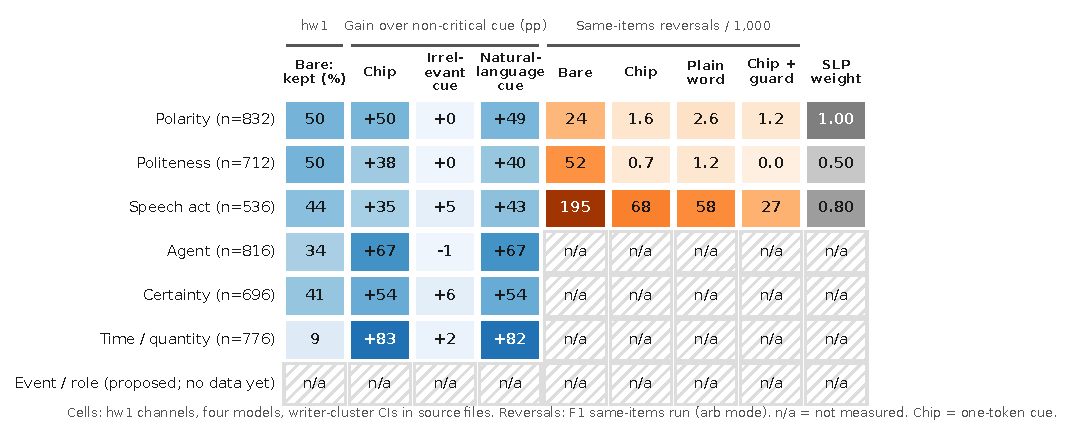
\includegraphics[width=\linewidth]{figs/fig4_dimension_table.pdf}
\caption{Dimension by intervention table. Left: share of bare outputs that keep the critical commitment (hw1, four models), and gain in that share over a non-critical cue for the chip, an irrelevant control cue and a natural-language cue. Right: same-items reversals per 1,000 messages for bare, chip, plain word and chip plus guard (\jmfOneUnits{} units; measured only for polarity, politeness and speech act), and the SLP severity weight (mean of two expert raters, $n=2$). Event/role structure is proposed but has no data. Every cell is printed; shading is redundant. Sources: \texttt{figs/figure\_values.json}.}\label{fig:table}
\Description{Dimension by intervention table.}
\end{figure}

\subsection{Cue Restoration Priced Per 1,000 Messages on the Same Items}\label{sec:price}

\paragraph{Design.}
The gains above come from constructed pairs. To price the cue on the messages that people actually shorten, we returned to the elicitation sample and took the \jmfOneUnits{} units whose source carried a cue that the human keywords dropped (polarity \jmfOneUnitsPol{}, politeness \jmfOneUnitsPolite{}, sentence type \jmfOneUnitsAct{}, the last a seeded subsample of question and request units). Each unit was regenerated by \jmfOneModels{} models (GPT-6.1-terra, Qwen2.5-7B, Llama-3.1-8B) under four arms at temperature zero: the stored bare output, the cue as a chip, the cue as a plain word, and the chip with the guard of \S\ref{sec:guard} monitoring the supplied chip. The restoration share is the proportion of units whose output honours the dropped cue; reversals per 1,000 messages are the exposure per 1,000 messages times one minus the restoration share. The bare arm reproduces the always-commit rates of \S\ref{sec:basecost}, so the unit construction matches. Disputed critical labels (\jmfOneArbRows{} rows) were resolved by the blind arbiter.

\paragraph{Results.}
Table~\ref{tab:price} gives the prices. Giving the cue on every message lowers polarity reversals from \jmfOneRevPolBare{} to \jmfOneRevPolChip{} (chip) or \jmfOneRevPolWord{} (word) per 1,000, and politeness reversals from \jmfOneRevPoliteBare{} to \jmfOneRevPoliteChip{} or \jmfOneRevPoliteWord{}. Chip and word are equivalent within 5 points on politeness (chip minus word \jmfOneChipMinusWordPolite{} points [\jmfOneChipMinusWordPoliteLo{}, \jmfOneChipMinusWordPoliteHi{}]) and not distinguishable on polarity (\jmfOneChipMinusWordPol{} [\jmfOneChipMinusWordPolLo{}, \jmfOneChipMinusWordPolHi{}]) or sentence type (\jmfOneChipMinusWordAct{} [\jmfOneChipMinusWordActLo{}, \jmfOneChipMinusWordActHi{}]). The guard on the chip arm helps on all three (polarity \jmfOneGuardGainPol{} points [\jmfOneGuardGainPolLo{}, \jmfOneGuardGainPolHi{}], politeness \jmfOneGuardGainPolite{} [\jmfOneGuardGainPoliteLo{}, \jmfOneGuardGainPoliteHi{}], sentence type \jmfOneGuardGainAct{} [\jmfOneGuardGainActLo{}, \jmfOneGuardGainActHi{}]); it raises the share of sentence-type units that honour the cue from \jmfOneRestActChip{}\% to \jmfOneRestActChipG{}\% [\jmfOneRestActChipGLo{}, \jmfOneRestActChipGHi{}]. Sentence type keeps the largest residual (\jmfOneRevActChipG{} [\jmfOneRevActChipGLo{}, \jmfOneRevActChipGHi{}] per 1,000 with chip and guard, from \jmfOneRevActBare{} bare), consistent with the speech-act dimension being the hardest in every earlier study.

\begin{table}[t]
\caption{Same-items price of the default and of cue restoration (\jmfOneUnits{} elicitation units, \jmfOneModels{} models, message-bootstrap 95\% intervals, arbiter-resolved labels). Each cell is the share of units whose output honours the dropped cue, followed by reversals per 1,000 messages if the arm is applied to every message and a cue is supplied each time. The price is the best case for the cue arms: it ignores the cost of cueing messages that need no cue and assumes the cue is elicited.}\label{tab:price}
\small
\begin{tabular}{lccccc}
\toprule
Dimension (units) & Quantity & Bare & Chip & Plain word & Chip + guard \\
\midrule
Polarity (\jmfOneUnitsPol{}) & Restored (\%) & \jmfOneRestPolBare{} & \jmfOneRestPolChip{} & \jmfOneRestPolWord{} & \jmfOneRestPolChipG{} \\
 & Reversals /1,000 & \jmfOneRevPolBare{} & \jmfOneRevPolChip{} [\jmfOneRevPolChipLo{}, \jmfOneRevPolChipHi{}] & \jmfOneRevPolWord{} [\jmfOneRevPolWordLo{}, \jmfOneRevPolWordHi{}] & \jmfOneRevPolChipG{} [\jmfOneRevPolChipGLo{}, \jmfOneRevPolChipGHi{}] \\
\addlinespace
Politeness (\jmfOneUnitsPolite{}) & Restored (\%) & \jmfOneRestPoliteBare{} & \jmfOneRestPoliteChip{} & \jmfOneRestPoliteWord{} & \jmfOneRestPoliteChipG{} \\
 & Reversals /1,000 & \jmfOneRevPoliteBare{} & \jmfOneRevPoliteChip{} [\jmfOneRevPoliteChipLo{}, \jmfOneRevPoliteChipHi{}] & \jmfOneRevPoliteWord{} [\jmfOneRevPoliteWordLo{}, \jmfOneRevPoliteWordHi{}] & \jmfOneRevPoliteChipG{} [\jmfOneRevPoliteChipGLo{}, \jmfOneRevPoliteChipGHi{}] \\
\addlinespace
Sentence type (\jmfOneUnitsAct{}) & Restored (\%) & \jmfOneRestActBare{} & \jmfOneRestActChip{} & \jmfOneRestActWord{} & \jmfOneRestActChipG{} \\
 & Reversals /1,000 & \jmfOneRevActBare{} & \jmfOneRevActChip{} [\jmfOneRevActChipLo{}, \jmfOneRevActChipHi{}] & \jmfOneRevActWord{} [\jmfOneRevActWordLo{}, \jmfOneRevActWordHi{}] & \jmfOneRevActChipG{} [\jmfOneRevActChipGLo{}, \jmfOneRevActChipGHi{}] \\
\bottomrule
\end{tabular}
\end{table}

\paragraph{A superseded estimate.}
An earlier version of this price transported the cue-honouring rate from the constructed pairs to the elicitation units. The measured rates do not match the transported ones for polarity or politeness (the transported rate was too optimistic for polarity and too pessimistic for politeness, in each case outside 5 points and outside the interval), so the measured rows replace the transported rows throughout.

\paragraph{Bound.}
Machine-judged outputs, three models, one prompt template, \jmfOneUnitsPol{} polarity units, and a price that assumes the cue is supplied. The restored outputs have no separate human check beyond the arbiter check (Section~\ref{sec:m-arbiter}).

% ------------------------------------------------------------------------------------------------
\subsection{Prior-Work Recap: The Commitment Guard}\label{sec:guard}

This subsection recaps the guard studies reported in our two earlier papers \cite{concurrent_se4all,concurrent_caleai}. It is subordinate to the writer-intent result: nothing in the argument of Section~\ref{sec:s4} depends on it, and the new material here is the human repair-usability audit (Section~\ref{sec:usability}) and the severity weighting (Section~\ref{sec:severity}).

\paragraph{Guard and baselines.}
The guard (G1) is a monitor on the output plus a bounded retry. The monitor flags an output that contradicts a supplied cue or that adds politeness the keywords do not carry; on a flag the model gets one short feedback turn that names the commitment it must keep, up to two retries at temperature zero, stopping at the first output the monitor does not flag. The monitor is a deterministic, rule-based extractor. A guard can look effective for a trivial reason, so we compare it with three alternatives that share the monitor, the trigger and the retry budget: a strip-only arm (G1s) that deletes an unsupplied ``please'' and makes no model call; a resample arm (G1r) that retries from the original prompt with no feedback at temperature $0.7$; and a feedback arm at temperature $0.7$ (G1t) that isolates feedback from decoding. The no-feedback baseline is G1r. The endpoint is a machine-scored partial predicate (the critical commitment and the absence of added politeness), not a usability judgement; usability is the subject of \S\ref{sec:usability}.

\paragraph{Transfer to fresh families (restated from our earlier papers).}
This result and the discovery-set guard result are reported in our earlier papers \cite{concurrent_se4all,concurrent_caleai}; we restate them here once, with the same frozen guard, because the audits below depend on them.
The frozen guard was applied, without change, to \jmgtFamilies{} fresh speech-act families that were not used to design it (\jmgtTargets{} target occurrences, \jmgwFlaggedF{} flagged requests). Joint pass rises from \jmgtJointP{}\% [\jmgtJointPLo{}, \jmgtJointPHi{}] to \jmgtJointG{}\% [\jmgtJointGLo{}, \jmgtJointGHi{}], a gain of \jmgwGain{} points [\jmgwGainLo{}, \jmgwGainHi{}]. Of the \jmgwStrictRepairN{} first-pass strict failures, \jmgwStrictRepairK{} (\jmgwStrictRepair{}\% [\jmgwStrictRepairLo{}, \jmgwStrictRepairHi{}]) are repaired; the guard rewrote \jmgwChangedK{} of \jmgwChangedN{} first-pass-correct targets and turned \jmgwPassToFailK{} passes into failures. The whole run took \jmgwGenCalls{} generation calls. On the discovery set the corresponding joint pass is \jmgbDiscPZero{}\% to \jmgbDiscGOne{}\% [\jmgbDiscGOneLo{}, \jmgbDiscGOneHi{}].

\paragraph{The no-feedback baseline.}
Table~\ref{tab:guard} compares the arms. Resampling without feedback gives about the strip-only gain on the fresh families (\jmgbWcGOner{}\% against \jmgbWcGOnes{}\%) and repairs \jmgbWcRepairGOner{}\% of strict failures against \jmgbWcRepairGOnes{}\% for the strip and \jmgbWcRepairGOne{}\% for the guard. The paired joint-pass contrast of the guard over the resample is \jmgbCWcGOneMGOner{} points [\jmgbCWcGOneMGOnerLo{}, \jmgbCWcGOneMGOnerHi{}] on the fresh families and \jmgbCDiscGOneMGOner{} [\jmgbCDiscGOneMGOnerLo{}, \jmgbCDiscGOneMGOnerHi{}] on the discovery set. Because the resample runs at temperature $0.7$ and the guard at zero, the clean contrast for the value of feedback is G1t minus G1r: \jmgbCWcGOnetMGOner{} points [\jmgbCWcGOnetMGOnerLo{}, \jmgbCWcGOnetMGOnerHi{}] on the fresh families and \jmgbCDiscGOnetMGOner{} [\jmgbCDiscGOnetMGOnerLo{}, \jmgbCDiscGOnetMGOnerHi{}] on discovery. Feedback adds value beyond resampling on both sets, and temperature is not what separates the guard from the baseline (G1 minus G1t: \jmgbCWcGOneMGOnet{} [\jmgbCWcGOneMGOnetLo{}, \jmgbCWcGOneMGOnetHi{}] on fresh families). The guard also beats the strip alone by \jmgwGOneMinusGOnes{} points [\jmgwGOneMinusGOnesLo{}, \jmgwGOneMinusGOnesHi{}], so the deletion explains part of the gain and not all of it.

\begin{table}[t]
\caption{The guard against its baselines (machine-scored joint pass, family-bootstrap 95\% intervals; strict repair is the share of first-pass strict failures repaired). Fresh families: \jmgbWcFamilies{} speech-act families, \jmgbWcTargets{} targets. Discovery: \jmgbDiscFamilies{} families, \jmgbDiscTargets{} targets. G1r is the no-feedback resample at temperature $0.7$.}\label{tab:guard}
\small
\begin{tabular}{lcccc}
\toprule
 & \multicolumn{2}{c}{Fresh families} & \multicolumn{2}{c}{Discovery} \\
\cmidrule(lr){2-3}\cmidrule(lr){4-5}
Arm & Joint pass (\%) & Strict repair & Joint pass (\%) & Strict repair \\
\midrule
First pass (P0) & \jmgbWcPZero{} [\jmgbWcPZeroLo{}, \jmgbWcPZeroHi{}] & --- & \jmgbDiscPZero{} [\jmgbDiscPZeroLo{}, \jmgbDiscPZeroHi{}] & --- \\
Strip only (G1s) & \jmgbWcGOnes{} [\jmgbWcGOnesLo{}, \jmgbWcGOnesHi{}] & \jmgbWcRepairGOnesK{}/\jmgbWcRepairGOnesN{} & \jmgbDiscGOnes{} [\jmgbDiscGOnesLo{}, \jmgbDiscGOnesHi{}] & \jmgbDiscRepairGOnesK{}/\jmgbDiscRepairGOnesN{} \\
Resample, no feedback (G1r) & \jmgbWcGOner{} [\jmgbWcGOnerLo{}, \jmgbWcGOnerHi{}] & \jmgbWcRepairGOnerK{}/\jmgbWcRepairGOnerN{} & \jmgbDiscGOner{} [\jmgbDiscGOnerLo{}, \jmgbDiscGOnerHi{}] & \jmgbDiscRepairGOnerK{}/\jmgbDiscRepairGOnerN{} \\
Feedback at $T=0.7$ (G1t) & \jmgbWcGOnet{} [\jmgbWcGOnetLo{}, \jmgbWcGOnetHi{}] & \jmgbWcRepairGOnetK{}/\jmgbWcRepairGOnetN{} & \jmgbDiscGOnet{} [\jmgbDiscGOnetLo{}, \jmgbDiscGOnetHi{}] & \jmgbDiscRepairGOnetK{}/\jmgbDiscRepairGOnetN{} \\
Guard (G1) & \jmgbWcGOne{} [\jmgbWcGOneLo{}, \jmgbWcGOneHi{}] & \jmgbWcRepairGOneK{}/\jmgbWcRepairGOneN{} & \jmgbDiscGOne{} [\jmgbDiscGOneLo{}, \jmgbDiscGOneHi{}] & \jmgbDiscRepairGOneK{}/\jmgbDiscRepairGOneN{} \\
\bottomrule
\end{tabular}
\end{table}

\paragraph{Bound.}
The endpoint is a machine-scored partial predicate on speech-act families; it supports the claim that the guard repairs commitment violations that a no-feedback retry does not, not a claim that its output is usable, fluent or preferred. Those questions are answered next, by people.

% ------------------------------------------------------------------------------------------------
\subsection{Repair Usability: A Blind Three-Rater Audit}\label{sec:usability}

\paragraph{Design.}
A guard that changes the text can make it worse to read. We audited this with a blind human audit under a decision rule frozen before any rating returned. The audit uses \jmpOneSevenItemsPerArm{} repaired texts and \jmpOneSevenItemsPerArm{} control texts (unrepaired outputs for which the monitor raised no flag, drawn from the same two pools), none of which had appeared in an earlier audit, rated by \jmpOneSevenRaters{} adult non-author classmates, \jmpOneSevenPerItem{} raters per item, with the arm hidden. The primary endpoint is the item-level majority of ``usable as the person's message''; secondary endpoints are meaning preserved against the keywords and cues and an invented stance or attitude. The frozen rule reads: if the interval for repaired minus control usable lies wholly below $-10$ points, the guard fails as a deployment clause; if it includes $-10$ but excludes zero, report a cost of uncertain size; if it includes zero, report no detectable cost. A comparison arm was added before any return to address the fact that controls never failed and repaired items did: the first-pass output that the guard replaced (\jmpOneSevenOrigItems{} items, each paired with its repair).

\paragraph{Result under the frozen rule.}
Repaired texts were usable in \jmpOneSevenRepUsableK{} of \jmpOneSevenRepUsableN{} items (\jmpOneSevenRepUsable{}\% [\jmpOneSevenRepUsableLo{}, \jmpOneSevenRepUsableHi{}]) and control texts in \jmpOneSevenCtlUsableK{} of \jmpOneSevenCtlUsableN{} (\jmpOneSevenCtlUsable{}\% [\jmpOneSevenCtlUsableLo{}, \jmpOneSevenCtlUsableHi{}]). The difference is \jmpOneSevenDiffUsable{} points [\jmpOneSevenDiffUsableLo{}, \jmpOneSevenDiffUsableHi{}]. The interval includes zero, so under the frozen rule the audit detects no usability cost, but the interval extends to \jmpOneSevenDiffUsableLo{} points: the audit is inconclusive, it neither shows nor excludes a cost, and it does not establish equivalence. Table~\ref{tab:p17} gives the endpoints. Repaired texts preserved the meaning less often than controls (\jmpOneSevenDiffPres{} points [\jmpOneSevenDiffPresLo{}, \jmpOneSevenDiffPresHi{}]) and so did the combined endpoint, usable and preserving (\jmpOneSevenDiffUsPres{} [\jmpOneSevenDiffUsPresLo{}, \jmpOneSevenDiffUsPresHi{}]); invented stance did not differ (\jmpOneSevenDiffStance{} [\jmpOneSevenDiffStanceLo{}, \jmpOneSevenDiffStanceHi{}]). The comparison is between inputs the first pass got wrong and inputs it got right, so the gap partly measures item difficulty and not the repair; the comparison against each repair's own failed original, below, holds the item fixed.

\begin{table}[t]
\caption{Blind audit of guard repairs (the repair-usability audit; \jmpOneSevenRaters{} raters, \jmpOneSevenPerItem{} per item, item-level strict majority; Wilson 95\% intervals for rates, Newcombe 95\% intervals for differences; preserving and stance exclude one item with no majority). The items are a pre-specified deterministic list, not a probability sample, so the rates describe these items.}\label{tab:p17}
\small
\begin{tabular}{lccc}
\toprule
Endpoint & Repaired & Control & Repaired $-$ control (points) \\
\midrule
Usable (primary) & \jmpOneSevenRepUsableK{}/\jmpOneSevenRepUsableN{} = \jmpOneSevenRepUsable{}\% [\jmpOneSevenRepUsableLo{}, \jmpOneSevenRepUsableHi{}] & \jmpOneSevenCtlUsableK{}/\jmpOneSevenCtlUsableN{} = \jmpOneSevenCtlUsable{}\% [\jmpOneSevenCtlUsableLo{}, \jmpOneSevenCtlUsableHi{}] & \jmpOneSevenDiffUsable{} [\jmpOneSevenDiffUsableLo{}, \jmpOneSevenDiffUsableHi{}] \\
Meaning preserved & \jmpOneSevenRepPresK{}/\jmpOneSevenRepPresN{} = \jmpOneSevenRepPres{}\% [\jmpOneSevenRepPresLo{}, \jmpOneSevenRepPresHi{}] & \jmpOneSevenCtlPresK{}/\jmpOneSevenCtlPresN{} = \jmpOneSevenCtlPres{}\% [\jmpOneSevenCtlPresLo{}, \jmpOneSevenCtlPresHi{}] & \jmpOneSevenDiffPres{} [\jmpOneSevenDiffPresLo{}, \jmpOneSevenDiffPresHi{}] \\
Invented stance & \jmpOneSevenRepStanceK{}/\jmpOneSevenRepStanceN{} = \jmpOneSevenRepStance{}\% [\jmpOneSevenRepStanceLo{}, \jmpOneSevenRepStanceHi{}] & \jmpOneSevenCtlStanceK{}/\jmpOneSevenCtlStanceN{} = \jmpOneSevenCtlStance{}\% [\jmpOneSevenCtlStanceLo{}, \jmpOneSevenCtlStanceHi{}] & \jmpOneSevenDiffStance{} [\jmpOneSevenDiffStanceLo{}, \jmpOneSevenDiffStanceHi{}] \\
\bottomrule
\end{tabular}
\end{table}

\paragraph{Against each repair's own failed original.}
Paired with the first-pass output that the guard replaced, repairs preserve the meaning more often (\jmpOneSevenOrigPres{} points [\jmpOneSevenOrigPresLo{}, \jmpOneSevenOrigPresHi{}], $p=\jmpOneSevenOrigPresP{}$ on \jmpOneSevenOrigPresPairs{} pairs) and invent a stance less often (\jmpOneSevenOrigStance{} points [\jmpOneSevenOrigStanceLo{}, \jmpOneSevenOrigStanceHi{}], $p=\jmpOneSevenOrigStanceP{}$ on \jmpOneSevenOrigStancePairs{} pairs). Usability shows no detectable change (\jmpOneSevenOrigUsable{} points [\jmpOneSevenOrigUsableLo{}, \jmpOneSevenOrigUsableHi{}], $p=\jmpOneSevenOrigUsableP{}$). Relative to the failed original, the repair preserves the meaning and removes the invented stance without a detectable change in how usable the sentence is.

\paragraph{Heterogeneity.}
Usability varies by the model that produced the repair. Gemma-3-4B repairs are usable in \jmpOneSevenRepGemmaUsableK{} of \jmpOneSevenRepGemmaUsableN{} (\jmpOneSevenRepGemmaUsable{}\%), against \jmpOneSevenRepLlamaUsableK{} of \jmpOneSevenRepLlamaUsableN{} for Llama-3.1-8B, \jmpOneSevenRepQwenSUsableK{} of \jmpOneSevenRepQwenSUsableN{} for Qwen2.5-7B and \jmpOneSevenRepTerraUsableK{} of \jmpOneSevenRepTerraUsableN{} for GPT-6.1-terra. These are descriptive counts on an unbalanced list. They suggest that a repair is only as readable as the repairing model's prose, which the pooled estimate hides.

\paragraph{Bound.}
\jmpOneSevenItemsPerArm{} items per arm from a fixed list, classmate raters rather than AAC users or clinicians, and a rule that detects no cost without excluding a cost of up to \jmpOneSevenDiffUsableLo{} points.

% ------------------------------------------------------------------------------------------------
\subsection{Weighting the Failures by Clinical Severity}\label{sec:severity}

Two speech-language pathologists, anonymous and paid as expert annotators of study materials, rated how serious each kind of silent meaning change would be if spoken as a client's message, and then rated stored outputs with the arm hidden: guard repairs (\jmslpAccRepairN{} ratings), the matching first-pass originals (\jmslpAccOrigN{}), chip outputs (\jmslpAccChipN{}) and plain-word outputs (\jmslpAccWordN{}); a rating is one rater's judgement of one output. This is an expert review with $n=2$ raters, not a population estimate, and the agreement statistics describe these two raters. Both rated negation dropped or added as the most serious change (\jmslpNegSeverity{} of 5) and both would block it (\jmslpNegBlock{}\%).

We weight each judge-flagged failure by the severity of its type, taking the largest weight on an output. On the fresh speech-act families the guard lowers the weighted failure rate from \jmslpWGuardBase{}\% to \jmslpWGuardG{}\% (strip only: \jmslpWGuardGs{}\%; unweighted \jmslpUGuardBase{}\% to \jmslpUGuardG{}\%; \jmslpWcN{} targets). On the human-written pairs the weighted failure rate is \jmslpWCueBare{}\% for bare keywords, \jmslpWCueChip{}\% with a chip and \jmslpWCueWord{}\% with a plain word, against \jmslpWCueIrrel{}\% with an irrelevant chip (\jmslpHwN{} rows per arm). The bare and irrelevant rates are inflated by the pair design, because two variants share one bare input; the comparison of interest is chip against word against the irrelevant control, and it again shows that the cue content carries the effect.

Rated directly, the SLPs judged the guard's repairs acceptable to speak as they stand in \jmslpAccRepair{}\% of ratings, and as they stand or after a small edit in \jmslpRepairEdit{}\%, against \jmslpAccOrig{}\% as they stand for the matching originals. Chip outputs were acceptable as they stand in \jmslpAccChip{}\% of ratings and plain-word outputs in \jmslpAccWord{}\%. The two raters agreed on whether an output says what the selected words mean on \jmslpAgreeA{}\% of items ($\kappa=\jmslpKappaA{}$) and on whether it is acceptable to speak on \jmslpAgreeB{}\% ($\kappa=\jmslpKappaB{}$); we report these as descriptions of this pair. The arms were rated on different numbers of items, so the acceptability figures are descriptive and do not rank the arms.

% ------------------------------------------------------------------------------------------------
\subsection{What These Studies Establish}\label{sec:establish}

The default is measurable, mostly attributable to a missing cue, and a supplied cue removes most of it on the dimensions measured. Against people's own keyword choices the affirmative default is the right guess for negation and costs about \jmtTwoRevPol{} silent reversals per 1,000 messages; it is not a prompt artefact and holds in \jmbreadthModels{} models from \jmbreadthFamilies{} families; a one-token cue or a plain word removes nearly all of the negation and politeness cost on the same items (to \jmfOneRevPolChip{} and \jmfOneRevPoliteChip{} per 1,000 with a chip); the cue's content, not its presence, does the work; and the guard (recapped in Section~\ref{sec:guard}) repairs violations that a no-feedback retry does not, and the blind repair audit could not exclude a usability cost (Section~\ref{sec:usability}). These results answer whether a commitment is preserved. Whether the preserved draft is the message the writer meant is a different question, which \S\ref{sec:waterfall} takes up with the writers themselves.
.
% Every number is a \jm... macro from make_macros.py (function s3() and earlier functions); no hand-typed numbers.
% Examples are stored outputs chosen by a declared rule (analysis/hw1/examples.md). Citations are limited to
% records already in refs.bib; nothing new was opened for this section.
% Labels defined here: sec:default (section), sec:basecost, sec:robust, sec:cue, sec:price, sec:asks, sec:guard, sec:usability, sec:severity.
% Needs \usepackage{booktabs} (acmart loads it).

\section{Studies and Results I: Defaults, Cue Restoration and the Guard}\label{sec:default}

This section reports the studies that establish what the default costs and what repairs it. Each study states its population, its estimator and its denominator, and each result is bounded once, where it is reported. We begin with the cost of the default measured against what people actually type (\S\ref{sec:basecost}), test whether the default belongs to the prompt or to the models (\S\ref{sec:robust}), show that a cue restores the commitment and that the cue's content is what does it (\S\ref{sec:cue}), price the restoration per 1,000 messages on the same items (\S\ref{sec:price}), ask whether any rule for when to ask beats chance (\S\ref{sec:asks}), and then evaluate the guard against a no-feedback baseline (\S\ref{sec:guard}), a blind human audit of its repairs (\S\ref{sec:usability}) and expert severity weights (\S\ref{sec:severity}).

\paragraph{Conventions common to all studies.}
Model outputs are labelled by two machine judges (J1, J2); disagreements on the critical commitment go to a blind arbiter that sees only the output text, and no label falls back to J1 when the arbiter is missing. Intervals are 95\% percentile bootstrap intervals clustered by writer (human-written pairs), by family (machine-written families and the guard) or by message (the elicitation sample). The human-written, legend, control and guard analyses use \jmconvBoot{} resamples with seed \jmconvSeed{}, the same-items study uses \jmconvBootFOne{} resamples with seed \jmconvSeedFOne{}, and the elicitation-sample prices and ask-policy contrasts use the resample counts stated in their reports. Rates ``per 1,000 messages'' are rates over the sampled units, not deployment rates. Where a decision rule governs a verdict (the legend test, the same-items comparisons, the guard baseline and the usability audit), it was written down and git-timestamped before the outcomes it governs were generated or returned; we do not call any of the studies pre-registered. Machine labels are used throughout this section; where a human check of the machine labels exists it is reported in the study that uses the labels, and the checks that have not yet returned are named as such.

% ------------------------------------------------------------------------------------------------
\subsection{What the Default Costs, Priced Against Human Base Rates}\label{sec:basecost}

\paragraph{Setting.}
A keyword string that omits a cue leaves the model to choose a reading, and the choice is a default. Whether a default is a good guess depends on how often the omitted cue was present in what the writer meant. We measured that base rate from people. The elicitation sample consists of \jmtTwoMessages{} source messages from an AAC-style corpus (\jmtTwoCorpus{} messages in total, of which \jmtTwoCorpusNeg{}\% are negated by a detector label), each shortened to keywords by three human keyword sets, giving \jmtTwoUnits{} keyword units. Stored outputs of \jmbreadthOrigModels{} generators were scored for three commitment dimensions (negation, politeness, sentence type), the dimensions for which a lexical test of ``the keywords carry the cue'' exists. The source cue labels are detector labels; these labels have no human check, so the prices below carry the detector's error and are provisional.

\paragraph{Affirmative is the right guess for negation; the cost is the asymmetry.}
Among keyword strings with no negation word, the source was negated in \jmtTwoPostPol{}\% [\jmtTwoPostPolLo{}, \jmtTwoPostPolHi{}] of cases (\jmtTwoPostBayesPol{}\% by Bayes' rule with the corpus prevalence; \jmtTwoPolRandHalf{}\% in the unweighted random half). Guessing the affirmative reading is therefore correct for all but a few messages in a hundred, and the models take it: they output an affirmative sentence for \jmtTwoAffGivenNoNeg{}\% of such inputs. The direction of the default is the rational one, which is consistent with prior reports that language models state negative content too positively \cite{chen2023say}; we do not present the default as new. What the base rate adds is the price. People dropped the negation word from \jmtTwoDroppedPol{}\% [\jmtTwoDroppedPolLo{}, \jmtTwoDroppedPolHi{}] of the negated messages, so an affirmative sentence silently reverses \jmtTwoRevPol{} [\jmtTwoRevPolLo{}, \jmtTwoRevPolHi{}] messages per 1,000, while a spurious negation is introduced in \jmtTwoSpurPol{} per 1,000. The affirmative guess breaks even with the opposite guess only if a reversed negation costs less than \jmtTwoBreakPol{} times a spurious one, and a prompt would have to be shown on about \jmtTwoQueriesPol{} inputs per reversal it prevents. The models' confidence also exceeds the evidence: they assert a negation on \jmtTwoModelCuePol{}\% of these inputs where the base rate is \jmtTwoPostPol{}\%.

\paragraph{Politeness and sentence type differ in kind.}
For politeness the default is calibrated: the source was polite in \jmtTwoPostPolite{}\% [\jmtTwoPostPoliteLo{}, \jmtTwoPostPoliteHi{}] of unmarked inputs and models add politeness to \jmtTwoModelCuePolite{}\%. Politeness the writer typed is lost for \jmtTwoRevPolite{} messages per 1,000, with a break-even ratio of \jmtTwoBreakPolite{}, so the asymmetry is milder than for negation; the opposite error, politeness added to a plain message, occurs in \jmtTwoSpurPolite{} per 1,000. For sentence type the statement default is not the Bayes-preferred guess at all: the source was a question, request or other non-statement in \jmtTwoPostAct{}\% [\jmtTwoPostActLo{}, \jmtTwoPostActHi{}] of unmarked inputs, while models assert one on only \jmtTwoModelCueAct{}\%, and \jmtTwoRevAct{} [\jmtTwoRevActLo{}, \jmtTwoRevActHi{}] messages per 1,000 have their sentence type reversed or flattened (break-even ratio \jmtTwoBreakAct{}: the statement default pays only if the two errors cost about the same).
Table~\ref{tab:basecost} collects these rows.

\begin{table}[t]
\caption{The default priced against human base rates (elicitation sample, \jmtTwoUnits{} keyword units from \jmtTwoMessages{} messages; Horvitz--Thompson weights; message-bootstrap 95\% intervals). Prior is the share of keyword strings without the cue whose source message carried it; model asserts cue is the share of such inputs for which the model's output asserts the cue-bearing value. Reversals are messages whose source has the cue, whose keywords lack it and whose output lacks it; the opposite error is an output that asserts the cue when the source lacks it; break-even is the cost ratio of a reversal to an opposite error at which the default stops paying. Source labels are detector labels.}\label{tab:basecost}
\footnotesize
\begin{tabular}{@{}lccccc@{}}
\toprule
Dimension & Prior [95\% CI] & Model asserts cue & Reversals /1,000 [CI] & Opposite /1,000 & Break-even \\
\midrule
Negation (affirmative default) & \jmtTwoPostPol{}\% [\jmtTwoPostPolLo{}, \jmtTwoPostPolHi{}] & \jmtTwoModelCuePol{}\% & \jmtTwoRevPol{} [\jmtTwoRevPolLo{}, \jmtTwoRevPolHi{}] & \jmtTwoSpurPol{} & \jmtTwoBreakPol{} \\
Politeness (plain default) & \jmtTwoPostPolite{}\% [\jmtTwoPostPoliteLo{}, \jmtTwoPostPoliteHi{}] & \jmtTwoModelCuePolite{}\% & \jmtTwoRevPolite{} [\jmtTwoRevPoliteLo{}, \jmtTwoRevPoliteHi{}] & \jmtTwoSpurPolite{} & \jmtTwoBreakPolite{} \\
Sentence type (statement default) & \jmtTwoPostAct{}\% [\jmtTwoPostActLo{}, \jmtTwoPostActHi{}] & \jmtTwoModelCueAct{}\% & \jmtTwoRevAct{} [\jmtTwoRevActLo{}, \jmtTwoRevActHi{}] & \jmtTwoSpurAct{} & \jmtTwoBreakAct{} \\
\bottomrule
\end{tabular}
\end{table}

\paragraph{The same default in human-written pairs.}
The human-written pairs (\S\ref{sec:cue}) test the default where the truth is known. Each pair differs in one commitment and shares one bare input, so a model that commits to one reading is wrong on exactly one variant and the true affirmative rate is 50\%. On the bare channel the models chose the affirmative reading in \jmtTwoHwAffShare{}\% of valid outputs.

\paragraph{Bound.}
Source cue labels are detector labels, the sentence-type ``no cue'' condition is a lexical proxy, the frame prevalence of negation (\jmtTwoPrevPol{}\%) exceeds the corpus value, and the prices are rates over a sampled elicitation frame. We therefore read the table as the cost structure of the default, not as a deployment rate.

% ------------------------------------------------------------------------------------------------
\paragraph{Appendix material.} The model-breadth tables and legend test (Appendix~\ref{sec:robust}) and the ask-policy arithmetic (Appendix~\ref{sec:asks}) are in the appendix; the main text uses only their headline results.

\subsection{A Cue Restores the Commitment, and the Content of the Cue Does It}\label{sec:cue}

\paragraph{Human-written pairs.}
To move beyond machine-written test items, \jmhwWritersTotal{} adult non-author classmates wrote sentence pairs that differ in one commitment and chose their own keywords; pairs were kept only after classmate checks, and \jmhwFamilies{} families were analysed, with \jmhwChipGainWriters{} to \jmhwAffShareWriters{} writers contributing to each contrast. Each family was expanded by \jmbreadthOrigModels{} models under bare keywords, a non-critical extra keyword, the cue as a one-token chip (for example \texttt{[NOT]}), the full cue set, and the full original text. The primary contrasts are those of the machine-written confirmation set (Holm-corrected over three); the human-written pairs are an exploratory replication of them. The chip gain over a non-critical word on speech act is \jmhwChipGain{} points [\jmhwChipGainLo{}, \jmhwChipGainHi{}] (\jmhwChipGainWriters{} writers, \jmhwChipGainFamilies{} families). When the full sentence is given, politeness is added to plain messages more often than it is removed from polite ones, by \jmhwPolGain{} points [\jmhwPolGainLo{}, \jmhwPolGainHi{}]. The bare affirmative share (\jmhwAffAll{}\%, \S\ref{sec:basecost}) is the third contrast. All three agree in direction and in decision with the machine-written confirmation set. Because each contrast rests on a handful of writers, we claim the direction and its consistency across writers and models, not the width of the intervals.

\paragraph{One stored case, by declared rule.}
The rule: order the analysed polarity families by the SHA-256 of the family identifier and take the first one in which a bare output commits to the wrong value while the chip output matches. That family is \texttt{hw-pol-075}, the model is Gemma-3-4B, and the target is the negated reading of ``The supervisor does not read my schedule.''

\begin{center}\small
\begin{tabular}{lll}
\toprule
Channel & Input & Stored output \\
\midrule
bare & \texttt{supervisor read} & ``The supervisor read.'' (affirmative) \\
chip & \texttt{[NOT] supervisor read} & ``The supervisor did not read.'' (negated) \\
\bottomrule
\end{tabular}
\end{center}

\noindent
In this dimension a bare output commits to the wrong value in \jmexPolBareWrong{}\% [\jmexPolBareWrongLo{}, \jmexPolBareWrongHi{}] of bare rows (the design ceiling), and when it does the chip output matches the target in \jmexPolRepair{}\% [\jmexPolRepairLo{}, \jmexPolRepairHi{}] of \jmexPolRepairN{} such rows. The same rule applied to speech act selects a family whose chip outputs match the target in a smaller share, \jmexActRepair{}\% [\jmexActRepairLo{}, \jmexActRepairHi{}] of \jmexActRepairN{} rows, in line with the larger residual for sentence type in \S\ref{sec:price}.

\paragraph{Six dimensions.}
Table~\ref{tab:sixdim} reports the cue gain for every measured dimension with its two controls. An irrelevant chip (a cue from another dimension, with the same token cost) adds about nothing on polarity, politeness, agent and time (at most \jmctlIrrelAddTime{} points) and a small amount on certainty (\jmctlIrrelAddCert{} [\jmctlIrrelAddCertLo{}, \jmctlIrrelAddCertHi{}]) and speech act (\jmctlIrrelAddAct{} [\jmctlIrrelAddActLo{}, \jmctlIrrelAddActHi{}]). The relevant chip beats the irrelevant chip by \jmctlOverIrrelAct{} to \jmctlOverIrrelTime{} points, so the gain is the content of the cue and not the presence of an extra token. A plain-language word delivers the same restoration as the chip within 5 points on every dimension except speech act; on speech act the word is better than the chip (chip minus word \jmctlOverWordAct{} points [\jmctlOverWordActLo{}, \jmctlOverWordActHi{}]). We do not claim that the chip is better than a plain word.

\begin{table}[t]
\caption{Cue restoration and its controls in human-written pairs (critical-commitment match, pooled over four models, writer-cluster 95\% intervals; points). Chip gain is chip minus non-critical word. Polarity and politeness bare matches sit at 50\% by design because both variants share one bare input; their informative quantity is the gain. Full input is the whole original sentence.}\label{tab:sixdim}
\small
\begin{tabular}{lccccc}
\toprule
Dimension & Bare match (\%) & Chip match (\%) & Chip gain [CI] & Irrelevant chip adds [CI] & Chip $-$ word [CI] \\
\midrule
Agent & \jmhwMatchBareAgent{} & \jmhwMatchChipAgent{} & \jmctlGAgent{} [\jmctlGAgentLo{}, \jmctlGAgentHi{}] & \jmctlIrrelAddAgent{} [\jmctlIrrelAddAgentLo{}, \jmctlIrrelAddAgentHi{}] & \jmctlOverWordAgent{} [\jmctlOverWordAgentLo{}, \jmctlOverWordAgentHi{}] \\
Time / quantity & \jmhwMatchBareTime{} & \jmhwMatchChipTime{} & \jmctlGTime{} [\jmctlGTimeLo{}, \jmctlGTimeHi{}] & \jmctlIrrelAddTime{} [\jmctlIrrelAddTimeLo{}, \jmctlIrrelAddTimeHi{}] & \jmctlOverWordTime{} [\jmctlOverWordTimeLo{}, \jmctlOverWordTimeHi{}] \\
Certainty & \jmhwMatchBareCert{} & \jmhwMatchChipCert{} & \jmctlGCert{} [\jmctlGCertLo{}, \jmctlGCertHi{}] & \jmctlIrrelAddCert{} [\jmctlIrrelAddCertLo{}, \jmctlIrrelAddCertHi{}] & \jmctlOverWordCert{} [\jmctlOverWordCertLo{}, \jmctlOverWordCertHi{}] \\
Polarity & \jmhwMatchBarePol{} & \jmhwMatchChipPol{} & \jmctlGPol{} [\jmctlGPolLo{}, \jmctlGPolHi{}] & \jmctlIrrelAddPol{} [\jmctlIrrelAddPolLo{}, \jmctlIrrelAddPolHi{}] & \jmctlOverWordPol{} [\jmctlOverWordPolLo{}, \jmctlOverWordPolHi{}] \\
Politeness & \jmhwMatchBarePolite{} & \jmhwMatchChipPolite{} & \jmctlGPolite{} [\jmctlGPoliteLo{}, \jmctlGPoliteHi{}] & \jmctlIrrelAddPolite{} [\jmctlIrrelAddPoliteLo{}, \jmctlIrrelAddPoliteHi{}] & \jmctlOverWordPolite{} [\jmctlOverWordPoliteLo{}, \jmctlOverWordPoliteHi{}] \\
Speech act & \jmhwMatchBareAct{} & \jmhwMatchChipAct{} & \jmctlGAct{} [\jmctlGActLo{}, \jmctlGActHi{}] & \jmctlIrrelAddAct{} [\jmctlIrrelAddActLo{}, \jmctlIrrelAddActHi{}] & \jmctlOverWordAct{} [\jmctlOverWordActLo{}, \jmctlOverWordActHi{}] \\
\bottomrule
\end{tabular}
\end{table}

\paragraph{Bound.}
\jmhwChipGainWriters{} to \jmhwAffShareWriters{} writers per dimension, one prompt template, and machine labels (with a blind arbiter for disputes); treated outputs have no separate human check beyond the arbiter check (Section~\ref{sec:m-arbiter}).

% ------------------------------------------------------------------------------------------------

\begin{figure}[t]
\centering
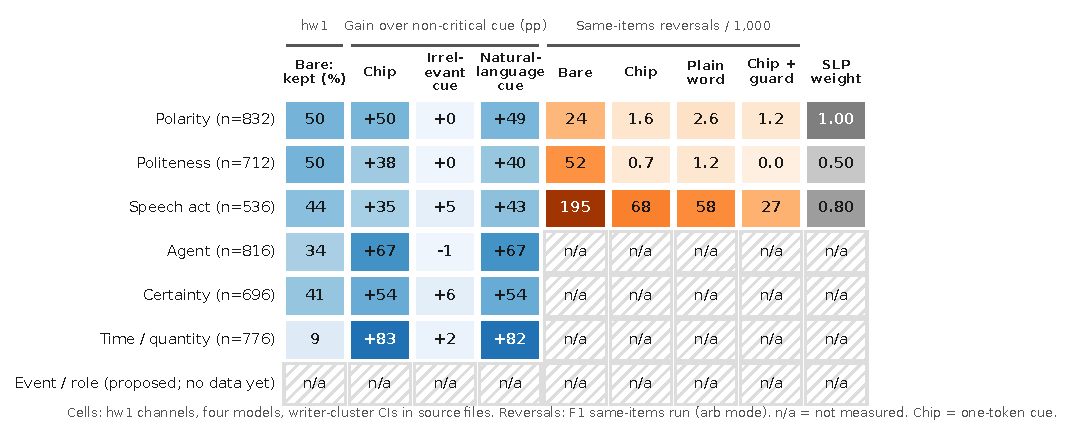
\includegraphics[width=\linewidth]{figs/fig4_dimension_table.pdf}
\caption{Dimension by intervention table. Left: share of bare outputs that keep the critical commitment (hw1, four models), and gain in that share over a non-critical cue for the chip, an irrelevant control cue and a natural-language cue. Right: same-items reversals per 1,000 messages for bare, chip, plain word and chip plus guard (\jmfOneUnits{} units; measured only for polarity, politeness and speech act), and the SLP severity weight (mean of two expert raters, $n=2$). Event/role structure is proposed but has no data. Every cell is printed; shading is redundant. Sources: \texttt{figs/figure\_values.json}.}\label{fig:table}
\Description{Dimension by intervention table.}
\end{figure}

\subsection{Cue Restoration Priced Per 1,000 Messages on the Same Items}\label{sec:price}

\paragraph{Design.}
The gains above come from constructed pairs. To price the cue on the messages that people actually shorten, we returned to the elicitation sample and took the \jmfOneUnits{} units whose source carried a cue that the human keywords dropped (polarity \jmfOneUnitsPol{}, politeness \jmfOneUnitsPolite{}, sentence type \jmfOneUnitsAct{}, the last a seeded subsample of question and request units). Each unit was regenerated by \jmfOneModels{} models (GPT-6.1-terra, Qwen2.5-7B, Llama-3.1-8B) under four arms at temperature zero: the stored bare output, the cue as a chip, the cue as a plain word, and the chip with the guard of \S\ref{sec:guard} monitoring the supplied chip. The restoration share is the proportion of units whose output honours the dropped cue; reversals per 1,000 messages are the exposure per 1,000 messages times one minus the restoration share. The bare arm reproduces the always-commit rates of \S\ref{sec:basecost}, so the unit construction matches. Disputed critical labels (\jmfOneArbRows{} rows) were resolved by the blind arbiter.

\paragraph{Results.}
Table~\ref{tab:price} gives the prices. Giving the cue on every message lowers polarity reversals from \jmfOneRevPolBare{} to \jmfOneRevPolChip{} (chip) or \jmfOneRevPolWord{} (word) per 1,000, and politeness reversals from \jmfOneRevPoliteBare{} to \jmfOneRevPoliteChip{} or \jmfOneRevPoliteWord{}. Chip and word are equivalent within 5 points on politeness (chip minus word \jmfOneChipMinusWordPolite{} points [\jmfOneChipMinusWordPoliteLo{}, \jmfOneChipMinusWordPoliteHi{}]) and not distinguishable on polarity (\jmfOneChipMinusWordPol{} [\jmfOneChipMinusWordPolLo{}, \jmfOneChipMinusWordPolHi{}]) or sentence type (\jmfOneChipMinusWordAct{} [\jmfOneChipMinusWordActLo{}, \jmfOneChipMinusWordActHi{}]). The guard on the chip arm helps on all three (polarity \jmfOneGuardGainPol{} points [\jmfOneGuardGainPolLo{}, \jmfOneGuardGainPolHi{}], politeness \jmfOneGuardGainPolite{} [\jmfOneGuardGainPoliteLo{}, \jmfOneGuardGainPoliteHi{}], sentence type \jmfOneGuardGainAct{} [\jmfOneGuardGainActLo{}, \jmfOneGuardGainActHi{}]); it raises the share of sentence-type units that honour the cue from \jmfOneRestActChip{}\% to \jmfOneRestActChipG{}\% [\jmfOneRestActChipGLo{}, \jmfOneRestActChipGHi{}]. Sentence type keeps the largest residual (\jmfOneRevActChipG{} [\jmfOneRevActChipGLo{}, \jmfOneRevActChipGHi{}] per 1,000 with chip and guard, from \jmfOneRevActBare{} bare), consistent with the speech-act dimension being the hardest in every earlier study.

\begin{table}[t]
\caption{Same-items price of the default and of cue restoration (\jmfOneUnits{} elicitation units, \jmfOneModels{} models, message-bootstrap 95\% intervals, arbiter-resolved labels). Each cell is the share of units whose output honours the dropped cue, followed by reversals per 1,000 messages if the arm is applied to every message and a cue is supplied each time. The price is the best case for the cue arms: it ignores the cost of cueing messages that need no cue and assumes the cue is elicited.}\label{tab:price}
\small
\begin{tabular}{lccccc}
\toprule
Dimension (units) & Quantity & Bare & Chip & Plain word & Chip + guard \\
\midrule
Polarity (\jmfOneUnitsPol{}) & Restored (\%) & \jmfOneRestPolBare{} & \jmfOneRestPolChip{} & \jmfOneRestPolWord{} & \jmfOneRestPolChipG{} \\
 & Reversals /1,000 & \jmfOneRevPolBare{} & \jmfOneRevPolChip{} [\jmfOneRevPolChipLo{}, \jmfOneRevPolChipHi{}] & \jmfOneRevPolWord{} [\jmfOneRevPolWordLo{}, \jmfOneRevPolWordHi{}] & \jmfOneRevPolChipG{} [\jmfOneRevPolChipGLo{}, \jmfOneRevPolChipGHi{}] \\
\addlinespace
Politeness (\jmfOneUnitsPolite{}) & Restored (\%) & \jmfOneRestPoliteBare{} & \jmfOneRestPoliteChip{} & \jmfOneRestPoliteWord{} & \jmfOneRestPoliteChipG{} \\
 & Reversals /1,000 & \jmfOneRevPoliteBare{} & \jmfOneRevPoliteChip{} [\jmfOneRevPoliteChipLo{}, \jmfOneRevPoliteChipHi{}] & \jmfOneRevPoliteWord{} [\jmfOneRevPoliteWordLo{}, \jmfOneRevPoliteWordHi{}] & \jmfOneRevPoliteChipG{} [\jmfOneRevPoliteChipGLo{}, \jmfOneRevPoliteChipGHi{}] \\
\addlinespace
Sentence type (\jmfOneUnitsAct{}) & Restored (\%) & \jmfOneRestActBare{} & \jmfOneRestActChip{} & \jmfOneRestActWord{} & \jmfOneRestActChipG{} \\
 & Reversals /1,000 & \jmfOneRevActBare{} & \jmfOneRevActChip{} [\jmfOneRevActChipLo{}, \jmfOneRevActChipHi{}] & \jmfOneRevActWord{} [\jmfOneRevActWordLo{}, \jmfOneRevActWordHi{}] & \jmfOneRevActChipG{} [\jmfOneRevActChipGLo{}, \jmfOneRevActChipGHi{}] \\
\bottomrule
\end{tabular}
\end{table}

\paragraph{A superseded estimate.}
An earlier version of this price transported the cue-honouring rate from the constructed pairs to the elicitation units. The measured rates do not match the transported ones for polarity or politeness (the transported rate was too optimistic for polarity and too pessimistic for politeness, in each case outside 5 points and outside the interval), so the measured rows replace the transported rows throughout.

\paragraph{Bound.}
Machine-judged outputs, three models, one prompt template, \jmfOneUnitsPol{} polarity units, and a price that assumes the cue is supplied. The restored outputs have no separate human check beyond the arbiter check (Section~\ref{sec:m-arbiter}).

% ------------------------------------------------------------------------------------------------
\subsection{Prior-Work Recap: The Commitment Guard}\label{sec:guard}

This subsection recaps the guard studies reported in our two earlier papers \cite{concurrent_se4all,concurrent_caleai}. It is subordinate to the writer-intent result: nothing in the argument of Section~\ref{sec:s4} depends on it, and the new material here is the human repair-usability audit (Section~\ref{sec:usability}) and the severity weighting (Section~\ref{sec:severity}).

\paragraph{Guard and baselines.}
The guard (G1) is a monitor on the output plus a bounded retry. The monitor flags an output that contradicts a supplied cue or that adds politeness the keywords do not carry; on a flag the model gets one short feedback turn that names the commitment it must keep, up to two retries at temperature zero, stopping at the first output the monitor does not flag. The monitor is a deterministic, rule-based extractor. A guard can look effective for a trivial reason, so we compare it with three alternatives that share the monitor, the trigger and the retry budget: a strip-only arm (G1s) that deletes an unsupplied ``please'' and makes no model call; a resample arm (G1r) that retries from the original prompt with no feedback at temperature $0.7$; and a feedback arm at temperature $0.7$ (G1t) that isolates feedback from decoding. The no-feedback baseline is G1r. The endpoint is a machine-scored partial predicate (the critical commitment and the absence of added politeness), not a usability judgement; usability is the subject of \S\ref{sec:usability}.

\paragraph{Transfer to fresh families (restated from our earlier papers).}
This result and the discovery-set guard result are reported in our earlier papers \cite{concurrent_se4all,concurrent_caleai}; we restate them here once, with the same frozen guard, because the audits below depend on them.
The frozen guard was applied, without change, to \jmgtFamilies{} fresh speech-act families that were not used to design it (\jmgtTargets{} target occurrences, \jmgwFlaggedF{} flagged requests). Joint pass rises from \jmgtJointP{}\% [\jmgtJointPLo{}, \jmgtJointPHi{}] to \jmgtJointG{}\% [\jmgtJointGLo{}, \jmgtJointGHi{}], a gain of \jmgwGain{} points [\jmgwGainLo{}, \jmgwGainHi{}]. Of the \jmgwStrictRepairN{} first-pass strict failures, \jmgwStrictRepairK{} (\jmgwStrictRepair{}\% [\jmgwStrictRepairLo{}, \jmgwStrictRepairHi{}]) are repaired; the guard rewrote \jmgwChangedK{} of \jmgwChangedN{} first-pass-correct targets and turned \jmgwPassToFailK{} passes into failures. The whole run took \jmgwGenCalls{} generation calls. On the discovery set the corresponding joint pass is \jmgbDiscPZero{}\% to \jmgbDiscGOne{}\% [\jmgbDiscGOneLo{}, \jmgbDiscGOneHi{}].

\paragraph{The no-feedback baseline.}
Table~\ref{tab:guard} compares the arms. Resampling without feedback gives about the strip-only gain on the fresh families (\jmgbWcGOner{}\% against \jmgbWcGOnes{}\%) and repairs \jmgbWcRepairGOner{}\% of strict failures against \jmgbWcRepairGOnes{}\% for the strip and \jmgbWcRepairGOne{}\% for the guard. The paired joint-pass contrast of the guard over the resample is \jmgbCWcGOneMGOner{} points [\jmgbCWcGOneMGOnerLo{}, \jmgbCWcGOneMGOnerHi{}] on the fresh families and \jmgbCDiscGOneMGOner{} [\jmgbCDiscGOneMGOnerLo{}, \jmgbCDiscGOneMGOnerHi{}] on the discovery set. Because the resample runs at temperature $0.7$ and the guard at zero, the clean contrast for the value of feedback is G1t minus G1r: \jmgbCWcGOnetMGOner{} points [\jmgbCWcGOnetMGOnerLo{}, \jmgbCWcGOnetMGOnerHi{}] on the fresh families and \jmgbCDiscGOnetMGOner{} [\jmgbCDiscGOnetMGOnerLo{}, \jmgbCDiscGOnetMGOnerHi{}] on discovery. Feedback adds value beyond resampling on both sets, and temperature is not what separates the guard from the baseline (G1 minus G1t: \jmgbCWcGOneMGOnet{} [\jmgbCWcGOneMGOnetLo{}, \jmgbCWcGOneMGOnetHi{}] on fresh families). The guard also beats the strip alone by \jmgwGOneMinusGOnes{} points [\jmgwGOneMinusGOnesLo{}, \jmgwGOneMinusGOnesHi{}], so the deletion explains part of the gain and not all of it.

\begin{table}[t]
\caption{The guard against its baselines (machine-scored joint pass, family-bootstrap 95\% intervals; strict repair is the share of first-pass strict failures repaired). Fresh families: \jmgbWcFamilies{} speech-act families, \jmgbWcTargets{} targets. Discovery: \jmgbDiscFamilies{} families, \jmgbDiscTargets{} targets. G1r is the no-feedback resample at temperature $0.7$.}\label{tab:guard}
\small
\begin{tabular}{lcccc}
\toprule
 & \multicolumn{2}{c}{Fresh families} & \multicolumn{2}{c}{Discovery} \\
\cmidrule(lr){2-3}\cmidrule(lr){4-5}
Arm & Joint pass (\%) & Strict repair & Joint pass (\%) & Strict repair \\
\midrule
First pass (P0) & \jmgbWcPZero{} [\jmgbWcPZeroLo{}, \jmgbWcPZeroHi{}] & --- & \jmgbDiscPZero{} [\jmgbDiscPZeroLo{}, \jmgbDiscPZeroHi{}] & --- \\
Strip only (G1s) & \jmgbWcGOnes{} [\jmgbWcGOnesLo{}, \jmgbWcGOnesHi{}] & \jmgbWcRepairGOnesK{}/\jmgbWcRepairGOnesN{} & \jmgbDiscGOnes{} [\jmgbDiscGOnesLo{}, \jmgbDiscGOnesHi{}] & \jmgbDiscRepairGOnesK{}/\jmgbDiscRepairGOnesN{} \\
Resample, no feedback (G1r) & \jmgbWcGOner{} [\jmgbWcGOnerLo{}, \jmgbWcGOnerHi{}] & \jmgbWcRepairGOnerK{}/\jmgbWcRepairGOnerN{} & \jmgbDiscGOner{} [\jmgbDiscGOnerLo{}, \jmgbDiscGOnerHi{}] & \jmgbDiscRepairGOnerK{}/\jmgbDiscRepairGOnerN{} \\
Feedback at $T=0.7$ (G1t) & \jmgbWcGOnet{} [\jmgbWcGOnetLo{}, \jmgbWcGOnetHi{}] & \jmgbWcRepairGOnetK{}/\jmgbWcRepairGOnetN{} & \jmgbDiscGOnet{} [\jmgbDiscGOnetLo{}, \jmgbDiscGOnetHi{}] & \jmgbDiscRepairGOnetK{}/\jmgbDiscRepairGOnetN{} \\
Guard (G1) & \jmgbWcGOne{} [\jmgbWcGOneLo{}, \jmgbWcGOneHi{}] & \jmgbWcRepairGOneK{}/\jmgbWcRepairGOneN{} & \jmgbDiscGOne{} [\jmgbDiscGOneLo{}, \jmgbDiscGOneHi{}] & \jmgbDiscRepairGOneK{}/\jmgbDiscRepairGOneN{} \\
\bottomrule
\end{tabular}
\end{table}

\paragraph{Bound.}
The endpoint is a machine-scored partial predicate on speech-act families; it supports the claim that the guard repairs commitment violations that a no-feedback retry does not, not a claim that its output is usable, fluent or preferred. Those questions are answered next, by people.

% ------------------------------------------------------------------------------------------------
\subsection{Repair Usability: A Blind Three-Rater Audit}\label{sec:usability}

\paragraph{Design.}
A guard that changes the text can make it worse to read. We audited this with a blind human audit under a decision rule frozen before any rating returned. The audit uses \jmpOneSevenItemsPerArm{} repaired texts and \jmpOneSevenItemsPerArm{} control texts (unrepaired outputs for which the monitor raised no flag, drawn from the same two pools), none of which had appeared in an earlier audit, rated by \jmpOneSevenRaters{} adult non-author classmates, \jmpOneSevenPerItem{} raters per item, with the arm hidden. The primary endpoint is the item-level majority of ``usable as the person's message''; secondary endpoints are meaning preserved against the keywords and cues and an invented stance or attitude. The frozen rule reads: if the interval for repaired minus control usable lies wholly below $-10$ points, the guard fails as a deployment clause; if it includes $-10$ but excludes zero, report a cost of uncertain size; if it includes zero, report no detectable cost. A comparison arm was added before any return to address the fact that controls never failed and repaired items did: the first-pass output that the guard replaced (\jmpOneSevenOrigItems{} items, each paired with its repair).

\paragraph{Result under the frozen rule.}
Repaired texts were usable in \jmpOneSevenRepUsableK{} of \jmpOneSevenRepUsableN{} items (\jmpOneSevenRepUsable{}\% [\jmpOneSevenRepUsableLo{}, \jmpOneSevenRepUsableHi{}]) and control texts in \jmpOneSevenCtlUsableK{} of \jmpOneSevenCtlUsableN{} (\jmpOneSevenCtlUsable{}\% [\jmpOneSevenCtlUsableLo{}, \jmpOneSevenCtlUsableHi{}]). The difference is \jmpOneSevenDiffUsable{} points [\jmpOneSevenDiffUsableLo{}, \jmpOneSevenDiffUsableHi{}]. The interval includes zero, so under the frozen rule the audit detects no usability cost, but the interval extends to \jmpOneSevenDiffUsableLo{} points: the audit is inconclusive, it neither shows nor excludes a cost, and it does not establish equivalence. Table~\ref{tab:p17} gives the endpoints. Repaired texts preserved the meaning less often than controls (\jmpOneSevenDiffPres{} points [\jmpOneSevenDiffPresLo{}, \jmpOneSevenDiffPresHi{}]) and so did the combined endpoint, usable and preserving (\jmpOneSevenDiffUsPres{} [\jmpOneSevenDiffUsPresLo{}, \jmpOneSevenDiffUsPresHi{}]); invented stance did not differ (\jmpOneSevenDiffStance{} [\jmpOneSevenDiffStanceLo{}, \jmpOneSevenDiffStanceHi{}]). The comparison is between inputs the first pass got wrong and inputs it got right, so the gap partly measures item difficulty and not the repair; the comparison against each repair's own failed original, below, holds the item fixed.

\begin{table}[t]
\caption{Blind audit of guard repairs (the repair-usability audit; \jmpOneSevenRaters{} raters, \jmpOneSevenPerItem{} per item, item-level strict majority; Wilson 95\% intervals for rates, Newcombe 95\% intervals for differences; preserving and stance exclude one item with no majority). The items are a pre-specified deterministic list, not a probability sample, so the rates describe these items.}\label{tab:p17}
\small
\begin{tabular}{lccc}
\toprule
Endpoint & Repaired & Control & Repaired $-$ control (points) \\
\midrule
Usable (primary) & \jmpOneSevenRepUsableK{}/\jmpOneSevenRepUsableN{} = \jmpOneSevenRepUsable{}\% [\jmpOneSevenRepUsableLo{}, \jmpOneSevenRepUsableHi{}] & \jmpOneSevenCtlUsableK{}/\jmpOneSevenCtlUsableN{} = \jmpOneSevenCtlUsable{}\% [\jmpOneSevenCtlUsableLo{}, \jmpOneSevenCtlUsableHi{}] & \jmpOneSevenDiffUsable{} [\jmpOneSevenDiffUsableLo{}, \jmpOneSevenDiffUsableHi{}] \\
Meaning preserved & \jmpOneSevenRepPresK{}/\jmpOneSevenRepPresN{} = \jmpOneSevenRepPres{}\% [\jmpOneSevenRepPresLo{}, \jmpOneSevenRepPresHi{}] & \jmpOneSevenCtlPresK{}/\jmpOneSevenCtlPresN{} = \jmpOneSevenCtlPres{}\% [\jmpOneSevenCtlPresLo{}, \jmpOneSevenCtlPresHi{}] & \jmpOneSevenDiffPres{} [\jmpOneSevenDiffPresLo{}, \jmpOneSevenDiffPresHi{}] \\
Invented stance & \jmpOneSevenRepStanceK{}/\jmpOneSevenRepStanceN{} = \jmpOneSevenRepStance{}\% [\jmpOneSevenRepStanceLo{}, \jmpOneSevenRepStanceHi{}] & \jmpOneSevenCtlStanceK{}/\jmpOneSevenCtlStanceN{} = \jmpOneSevenCtlStance{}\% [\jmpOneSevenCtlStanceLo{}, \jmpOneSevenCtlStanceHi{}] & \jmpOneSevenDiffStance{} [\jmpOneSevenDiffStanceLo{}, \jmpOneSevenDiffStanceHi{}] \\
\bottomrule
\end{tabular}
\end{table}

\paragraph{Against each repair's own failed original.}
Paired with the first-pass output that the guard replaced, repairs preserve the meaning more often (\jmpOneSevenOrigPres{} points [\jmpOneSevenOrigPresLo{}, \jmpOneSevenOrigPresHi{}], $p=\jmpOneSevenOrigPresP{}$ on \jmpOneSevenOrigPresPairs{} pairs) and invent a stance less often (\jmpOneSevenOrigStance{} points [\jmpOneSevenOrigStanceLo{}, \jmpOneSevenOrigStanceHi{}], $p=\jmpOneSevenOrigStanceP{}$ on \jmpOneSevenOrigStancePairs{} pairs). Usability shows no detectable change (\jmpOneSevenOrigUsable{} points [\jmpOneSevenOrigUsableLo{}, \jmpOneSevenOrigUsableHi{}], $p=\jmpOneSevenOrigUsableP{}$). Relative to the failed original, the repair preserves the meaning and removes the invented stance without a detectable change in how usable the sentence is.

\paragraph{Heterogeneity.}
Usability varies by the model that produced the repair. Gemma-3-4B repairs are usable in \jmpOneSevenRepGemmaUsableK{} of \jmpOneSevenRepGemmaUsableN{} (\jmpOneSevenRepGemmaUsable{}\%), against \jmpOneSevenRepLlamaUsableK{} of \jmpOneSevenRepLlamaUsableN{} for Llama-3.1-8B, \jmpOneSevenRepQwenSUsableK{} of \jmpOneSevenRepQwenSUsableN{} for Qwen2.5-7B and \jmpOneSevenRepTerraUsableK{} of \jmpOneSevenRepTerraUsableN{} for GPT-6.1-terra. These are descriptive counts on an unbalanced list. They suggest that a repair is only as readable as the repairing model's prose, which the pooled estimate hides.

\paragraph{Bound.}
\jmpOneSevenItemsPerArm{} items per arm from a fixed list, classmate raters rather than AAC users or clinicians, and a rule that detects no cost without excluding a cost of up to \jmpOneSevenDiffUsableLo{} points.

% ------------------------------------------------------------------------------------------------
\subsection{Weighting the Failures by Clinical Severity}\label{sec:severity}

Two speech-language pathologists, anonymous and paid as expert annotators of study materials, rated how serious each kind of silent meaning change would be if spoken as a client's message, and then rated stored outputs with the arm hidden: guard repairs (\jmslpAccRepairN{} ratings), the matching first-pass originals (\jmslpAccOrigN{}), chip outputs (\jmslpAccChipN{}) and plain-word outputs (\jmslpAccWordN{}); a rating is one rater's judgement of one output. This is an expert review with $n=2$ raters, not a population estimate, and the agreement statistics describe these two raters. Both rated negation dropped or added as the most serious change (\jmslpNegSeverity{} of 5) and both would block it (\jmslpNegBlock{}\%).

We weight each judge-flagged failure by the severity of its type, taking the largest weight on an output. On the fresh speech-act families the guard lowers the weighted failure rate from \jmslpWGuardBase{}\% to \jmslpWGuardG{}\% (strip only: \jmslpWGuardGs{}\%; unweighted \jmslpUGuardBase{}\% to \jmslpUGuardG{}\%; \jmslpWcN{} targets). On the human-written pairs the weighted failure rate is \jmslpWCueBare{}\% for bare keywords, \jmslpWCueChip{}\% with a chip and \jmslpWCueWord{}\% with a plain word, against \jmslpWCueIrrel{}\% with an irrelevant chip (\jmslpHwN{} rows per arm). The bare and irrelevant rates are inflated by the pair design, because two variants share one bare input; the comparison of interest is chip against word against the irrelevant control, and it again shows that the cue content carries the effect.

Rated directly, the SLPs judged the guard's repairs acceptable to speak as they stand in \jmslpAccRepair{}\% of ratings, and as they stand or after a small edit in \jmslpRepairEdit{}\%, against \jmslpAccOrig{}\% as they stand for the matching originals. Chip outputs were acceptable as they stand in \jmslpAccChip{}\% of ratings and plain-word outputs in \jmslpAccWord{}\%. The two raters agreed on whether an output says what the selected words mean on \jmslpAgreeA{}\% of items ($\kappa=\jmslpKappaA{}$) and on whether it is acceptable to speak on \jmslpAgreeB{}\% ($\kappa=\jmslpKappaB{}$); we report these as descriptions of this pair. The arms were rated on different numbers of items, so the acceptability figures are descriptive and do not rank the arms.

% ------------------------------------------------------------------------------------------------
\subsection{What These Studies Establish}\label{sec:establish}

The default is measurable, mostly attributable to a missing cue, and a supplied cue removes most of it on the dimensions measured. Against people's own keyword choices the affirmative default is the right guess for negation and costs about \jmtTwoRevPol{} silent reversals per 1,000 messages; it is not a prompt artefact and holds in \jmbreadthModels{} models from \jmbreadthFamilies{} families; a one-token cue or a plain word removes nearly all of the negation and politeness cost on the same items (to \jmfOneRevPolChip{} and \jmfOneRevPoliteChip{} per 1,000 with a chip); the cue's content, not its presence, does the work; and the guard (recapped in Section~\ref{sec:guard}) repairs violations that a no-feedback retry does not, and the blind repair audit could not exclude a usability cost (Section~\ref{sec:usability}). These results answer whether a commitment is preserved. Whether the preserved draft is the message the writer meant is a different question, which \S\ref{sec:waterfall} takes up with the writers themselves.

% Section 4: Studies and Results II (writer-grounded validity; necessary but not sufficient; event/role structure;
% consultant-revised requirements; frontier limits). Every number is a \jm... macro from make_macros.py (function s4(), plus
% earlier functions). No hand-typed numbers. Quoted examples are stored outputs chosen by a declared rule, printed with their rate.
% Labels provided: sec:s4, sec:waterfall, sec:whole-message, sec:event-role, sec:validity, sec:slp, sec:req-revisions, sec:frontier.
% Cross-references used from other sections: sec:default, sec:guard, sec:design, sec:req.
% CITE-NEEDED (not opened, not in refs.bib): CLAM / Clarify When Necessary (Zhang and Choi, NAACL Findings 2025); COMPA (CHI 2024);
%   semantic entropy (Kuhn et al.; Farquhar et al.); contextual calibration (Zhao et al. 2021).
\section{Studies and Results II: Writer-Grounded Validity and the Limits of Commitment Preservation}\label{sec:s4}

Section~\ref{sec:default} and Section~\ref{sec:guard} establish that a missing cue is the main source of silent reversals and that a supplied cue, or a guard that deletes an unlicensed addition, removes most of them.
Those results are measured against a critical commitment: the one dimension that a minimal pair contrasts, labelled by automatic judges and a blind arbiter.
This section asks whether that measurement tracks what the people who write and use the messages mean by a correct draft.
It reports the studies in turn and then a set of bounded negative results.
In the writer-intent study (writer-intent study) the \jmpOneEightWriters{} writers of the human-written pairs rated drafts generated from their own pairs.
A whole-message analysis of those ratings separates the reasons a draft is rejected.
A human check of the arbitrated labels (arbiter check) measures how well each automatic judge and the arbiter agree with people.
Speech-language pathologists (SLPs; \jmdesignSlp{} raters) supply clinical severity weights and an acceptability review.
Two paid design consultants who use AAC (\jmdesignConsultants{} consultants) revise the requirement list; we know nothing of their communication or access method beyond that they use AAC, and nothing they said is treated as data.
The section closes with the frontier results that mark where asking, model uncertainty and partner context stop helping.
The result that organises the section is that preserving the critical commitment is necessary and far from sufficient, and that the shortfall has a specific structure.

\subsection{Writer-intent study}\label{sec:waterfall}

\paragraph{Design.}
Each of the \jmpOneEightWriters{} writers rated \jmpOneEightPerWriter{} drafts generated from their own kept pairs, half from the keywords alone (\emph{bare}) and half from the keywords plus the chip for the critical dimension (\emph{chip}).
Drafts came from the \jmwmModels{} primary models under the base prompt, and the draw was seeded and fixed before rating (\jmpOneEightAcceptN{} drafts in all).
For each draft the writer said which of their own two sentences it expresses (their sentence A, their sentence B, something else, or unclear) and whether they would accept it as their message (yes, yes with a small edit, or no), with a free-text note.
Writers were adult non-author university classmates who consented and were paid; the study measures writer-intent agreement, not validation by AAC users.
The automatic judge labels only the critical dimension, whereas the writer judges the whole message.
In the bare channel the keywords do not say which sentence the writer meant, so no model could know; the bare match rate is a reference level, not a failure rate, and the cue effect below is the measured value of supplying the missing commitment, not a claim that the chip is sufficient.

\paragraph{Results.}
Table~\ref{tab:s4-p18} gives the ratings.
Writers said the draft expressed the sentence the pair was generated from in \jmpOneEightMatchAll{}\% of rated drafts (\jmpOneEightMatchAllK{} of \jmpOneEightMatchAllN{}; 95\% interval \jmpOneEightMatchAllLo{} to \jmpOneEightMatchAllHi{}), and in \jmpOneEightElse{}\% they said it expressed something else.
The chip raises the intended-version match from \jmpOneEightMatchBare{}\% to \jmpOneEightMatchChip{}\%, a gain of \jmpOneEightCueGain{} points (writer-cluster interval \jmpOneEightCueGainLo{} to \jmpOneEightCueGainHi{}).
Writers accepted \jmpOneEightAcceptYesK{} of \jmpOneEightAcceptN{} drafts as written, and the one accepted draft came from the bare channel; \jmpOneEightAcceptYesSmall{}\% were acceptable as written or with a small edit.
Writers' agreement with the automatic judge on the four-way label (A, B, other, unclear) was \jmpOneEightAgreeFour{}\% ($\kappa$ = \jmpOneEightKappa{}).

\begin{table}[t]
\centering\small
\caption{Writer ratings of drafts generated from their own pairs (writer-intent study). Match: the writer says the draft expresses the sentence it was generated from. Bare is a reference level because the keywords do not determine the side. Intervals are 95\% Wilson over drafts; the cue contrast uses writer clusters.}\label{tab:s4-p18}
\begin{tabular}{@{}lrrrr@{}}
\toprule
Channel & Drafts & Match (\%) & Accepted as written & As written or small edit (\%) \\
\midrule
Bare & \jmpOneEightYesBareN{} & \jmpOneEightMatchBare{} [\jmpOneEightMatchBareLo{}, \jmpOneEightMatchBareHi{}] & \jmpOneEightYesBareK{} of \jmpOneEightYesBareN{} & \jmpOneEightSmallBare{} \\
Chip & \jmpOneEightYesChipN{} & \jmpOneEightMatchChip{} [\jmpOneEightMatchChipLo{}, \jmpOneEightMatchChipHi{}] & \jmpOneEightYesChipK{} of \jmpOneEightYesChipN{} & \jmpOneEightSmallChip{} \\
All & \jmpOneEightAcceptN{} & \jmpOneEightMatchAll{} [\jmpOneEightMatchAllLo{}, \jmpOneEightMatchAllHi{}] & \jmpOneEightAcceptYesK{} of \jmpOneEightAcceptN{} & \jmpOneEightAcceptYesSmall{} \\
\bottomrule
\end{tabular}
\end{table}

\paragraph{Is the acceptance criterion too strict?}
Two criteria are used on purpose and both are reported. ``Intended version'' asks whether the draft is the sentence the writer wrote, and ``accepted as written'' asks whether the writer would send it unchanged; both are strict, and the writer's own sentence contained words absent from the keywords in \jmwmDroppedUnrecShare{}\% of rejections, so some rejection is built into keyword input. A graded reading is therefore the better summary of how far drafts are from usable: \jmpOneEightAcceptYesSmall{}\% of drafts (\jmpOneEightAcceptYesSmallK{} of \jmpOneEightAcceptN{}) were acceptable as written or with a small edit, against \jmpOneEightAcceptNo{}\% (\jmpOneEightAcceptNoK{}) that the writer would not accept. The claim that commitment preservation is necessary but not sufficient does not rest on the strict criterion: it holds under the graded one, because the share needing no or a small edit is far below the share of drafts that keep the critical commitment. We did not collect an edit-distance measure, and we have not tested how many edits writers could make with the interface they would use.

\paragraph{From a correct commitment to an accepted draft.}
Table~\ref{tab:s4-waterfall} follows the drafts through three filters.
The judge marked the critical commitment correct in \jmwmRightN{} of \jmwmAllN{} drafts (\jmwmRightShare{}\%).
Among those, writers said the draft was the version they meant in \jmwmRightIntendedK{} of \jmwmRightIntendedN{} cases with an answer (\jmwmRightIntShare{}\%), and accepted \jmwmRightAccK{} as written.
The other direction is clean: where the judge marked the critical commitment wrong, the writer said the draft was not the intended version in \jmwmWrongNotIntK{} of \jmwmWrongNotIntN{} cases.
The automatic judge's failures are therefore real failures to the people who wrote the messages, and its passes are not sufficient.

\begin{table}[t]
\centering\small
\caption{From a correct critical commitment to an accepted draft (writer-intent study). Denominators are stated in each cell because some writer answers are unknown.}\label{tab:s4-waterfall}
\begin{tabular}{@{}lrrr@{}}
\toprule
 & All & Chip & Bare \\
\midrule
Drafts rated & \jmwmAllN{} & \jmpOneEightYesChipN{} & \jmpOneEightYesBareN{} \\
Judge: critical commitment correct & \jmwmRightN{} & \jmwmRightChipN{} & \jmwmRightBareN{} \\
\ \ and writer: it is the intended version & \jmwmRightIntendedK{} of \jmwmRightIntendedN{} & \jmwmRightChipIntK{} of \jmwmRightChipIntN{} & \jmwmRightBareIntK{} of \jmwmRightBareIntN{} \\
\ \ and writer: accepted as written & \jmwmRightAccK{} of \jmwmRightN{} & \jmwmRightChipAccK{} of \jmwmRightChipN{} & \jmwmRightBareAccK{} of \jmwmRightBareN{} \\
\bottomrule
\end{tabular}
\end{table}


\begin{figure}[t]
\centering
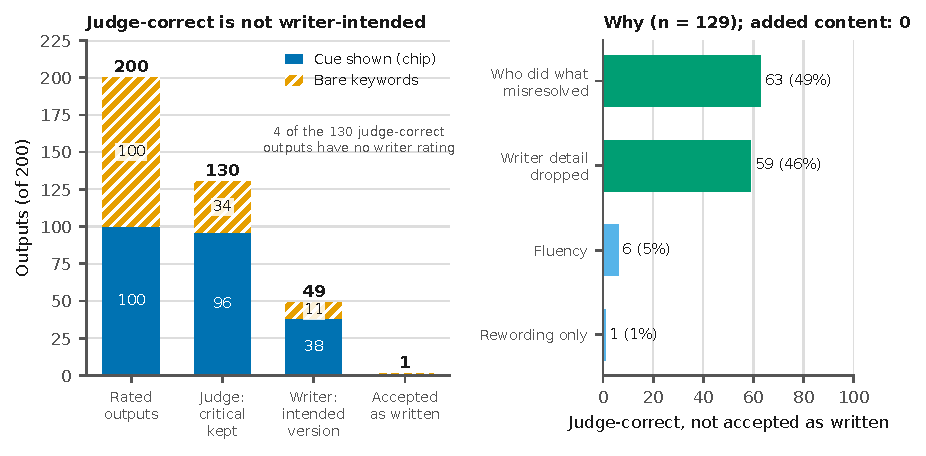
\includegraphics[width=\linewidth]{figs/fig2_waterfall.pdf}
\caption{Judge-correct is not writer-intended. Left: of \jmpOneEightAcceptN{} writer-rated outputs, \jmwmRightN{} keep the critical commitment by the judge, \jmwmRightIntendedK{} of the \jmwmRightIntendedN{} with a writer rating are the writer's intended version, and \jmpOneEightAcceptYesK{} is accepted as written. Right: reasons among the judge-correct outputs not accepted as written (writer-coded classification, kappa \jmwmHandKappa{} on a 40-item hand check); no output was coded as adding content.}\label{fig:waterfall}
\Description{Judge-correct is not writer-intended.}
\end{figure}

\subsection{Why correct drafts are rejected: the whole-message analysis}\label{sec:whole-message}

\paragraph{Method.}
For each of the \jmwmAllNotAccN{} drafts that writers did not accept as written, we assigned a primary reason from the writer's note and a lexical diff between the draft and the writer's own sentence: the critical commitment is wrong, a different event or role is expressed (substitution), writer detail is missing (dropped), content is added, the draft is not fluent, or it only rewords.
The analysis is post hoc and used no new model calls.
The diff classifier agrees with a hand coding of \jmwmHandN{} drafts in \jmwmHandAgree{}\% of cases ($\kappa$ = \jmwmHandKappa{}); the hand coder was an LLM and the classifier rules were written after seeing those drafts, so the agreement is an optimistic bound rather than a held-out estimate.
A second flag marks whether a content word of the writer's sentence is neither among the keywords nor a chip realisation, so that the model could not have known it.

\paragraph{Reasons.}
Table~\ref{tab:s4-reasons} gives the primary reasons by channel.
Without the cue, \jmwmBareCritical{}\% of non-accepted drafts fail on the critical commitment itself; with the chip that share falls to \jmwmChipCritical{}\%.
The cue converts violations into the two failures that remain: substitution (\jmwmChipSubst{}\%) and dropped writer detail (\jmwmChipDropped{}\%) among chip drafts.
Restricting to drafts whose critical commitment the judge marked correct and the writer did not accept as written (\jmwmRightNotAccN{} drafts), the primary reason is substitution in \jmwmRightSubst{}\% and dropped detail in \jmwmRightDropped{}\%; fluency accounts for \jmwmRightFluency{}\%.
Among the \jmwmROneN{} judge-correct drafts that writers said were not the intended version, \jmwmROneSubstK{} (\jmwmROneSubst{}\%) are substitutions and \jmwmROneDroppedK{} (\jmwmROneDropped{}\%) are dropped detail.

\begin{table}[t]
\centering\small
\caption{Primary reason a draft was not accepted as written (writer-intent study; share of non-accepted drafts; classifier validated against a hand coding, agreement \jmwmHandAgree{}\%). Fluency and rewording account for the remainder.}\label{tab:s4-reasons}
\begin{tabular}{@{}lrrr@{}}
\toprule
Primary reason & Bare (n=\jmwmBareNotAccN{}) & Chip (n=\jmwmChipNotAccN{}) & All (n=\jmwmAllNotAccN{}) \\
\midrule
Critical commitment wrong & \jmwmBareCritical{} & \jmwmChipCritical{} & \jmwmAllCritical{} \\
Event or role substituted & \jmwmBareSubst{} & \jmwmChipSubst{} & \jmwmAllSubst{} \\
Writer detail dropped & \jmwmBareDropped{} & \jmwmChipDropped{} & \jmwmAllDropped{} \\
Content added & --- & --- & \jmwmAdded{} \\
\bottomrule
\end{tabular}
\end{table}

\paragraph{Compression loss.}
In \jmwmRightUnrec{}\% of the judge-correct, non-accepted drafts the writer's sentence contains at least one content word that is neither a keyword nor a chip realisation.
The writers typed keywords because typing is slow; the details they meant (a place, a time, an object) were not in the input.
A draft is therefore a plausible completion of a compressed message and not a reconstruction of it, and the shortfall is a property of the task before it is a property of any model.
The appropriate response is a draft the writer can inspect, choose among and edit, which is the design the consultants asked for (Section~\ref{sec:req-revisions}).

\paragraph{Added content.}
Added content is never the primary reason for rejection in the writer data (\jmwmAdded{}\% of primary reasons).
As a secondary flag, \jmwmRightAddedFlag{}\% of judge-correct, non-accepted drafts contain a content word absent from the input.
We therefore do not claim that these drafts add unrequested content as the reason writers reject them.
The SLP panel applies a different standard, whether a sentence is safe to speak as a client's message with no writer sentence available, and there added content is prominent (Section~\ref{sec:slp}).

\paragraph{A deployable signal.}
Among judge-correct drafts, the ratio of draft length to the number of keywords given ranks the drafts that writers reject with AUROC \jmwmLenAuc{} (item-bootstrap interval \jmwmLenAucLo{} to \jmwmLenAucHi{}).
The critical label alone ranks writer rejection over all drafts at AUROC \jmwmCritAuc{}; the label plus three deployable features (judge added-content flag, length ratio, novel content words) reaches \jmwmCritPlusAuc{} (\jmwmCritPlusAucLo{} to \jmwmCritPlusAucHi{}) under cross-validation.
This is an observational association in \jmwmAllN{} drafts from \jmpOneEightWriters{} writers and identifies the drafts that say much more than the keywords gave; it is not a validated quality metric.

\paragraph{Examples.}
Table~\ref{tab:s4-examples} shows stored outputs chosen by a declared rule: among judge-correct drafts that writers said were not the intended version, for each primary reason the draft with the smallest SHA-256 of a fixed string and the item identifier.
The first two rows are writer-grounded; the last two are from the SLP panel, drawn by the same rule among judge-passed outputs that an SLP marked partly or no.

\begin{table*}[t]
\centering\small
\caption{Real stored outputs by declared rule. Rates: substitution \jmwmROneSubstK{} of \jmwmROneN{} and dropped \jmwmROneDroppedK{} of \jmwmROneN{} judge-correct drafts the writer said were not the intended version; SLP substitution \jmwmSlpSubstK{} and added \jmwmSlpAddedK{} of \jmwmSlpReasonN{} judge-passed rater-items marked partly or no.}\label{tab:s4-examples}
\begin{tabular}{@{}p{0.09\linewidth}p{0.17\linewidth}p{0.24\linewidth}p{0.2\linewidth}p{0.22\linewidth}@{}}
\toprule
Reason & Input & Writer's sentence or judgement & Draft & Note \\
\midrule
Substitution & \texttt{[SURE] taxi wait} & ``The taxi waits outside the main gate.'' & ``I am sure I need to wait for the taxi.'' & ``I wait for the taxi rather than the taxi waiting at the gate.'' \\
Dropped & \texttt{[SURE] soup warm} & ``The soup is warm in the kitchen.'' & ``The soup is definitely warm.'' & ``Adds definite certainty and omits the kitchen.'' \\
SLP: substitution & \texttt{[TELL] bus stop hospital} & SLP: says what was selected, no; acceptable, no & ``I need to go to the hospital from the bus stop.'' & ``Invents the speaker needing hospital travel instead of stating something about the bus stopping at the hospital.'' \\
SLP: added & \texttt{please put soup bowl} & SLP: partly; acceptable with edit & ``Please put the soup bowl on the table.'' & ``Remove the invented table; confirm soup into a bowl versus moving a soup bowl.'' \\
\bottomrule
\end{tabular}
\end{table*}

\subsection{Event and role structure as a commitment dimension}\label{sec:event-role}

The commitment vector used so far has \jmdesignDims{} dimensions.
The whole-message analysis shows a failure that none of them names: the draft says something that is fluent, keeps the negation, the speech act and the tone, and nevertheless assigns the wrong participants to the wrong event.
``I am sure I need to wait for the taxi'' keeps the certainty chip and changes who does what.
We propose event and role structure as an additional commitment dimension, defined as the event the message describes and the participants that fill its roles (who acts, who or what is acted on, where or for whom), including the event to which a negation or modal attaches.
It differs from the existing agent dimension in scope: agent covers who performs the stated action, whereas event and role structure covers whether the action, its participants and its negation scope are the ones the writer meant.
Because the judge labels only the dimension a pair contrasts, a role error on an item whose contrast is certainty is not counted.

Three independent sources point to the same dimension.
First, substitution is the leading primary reason among judge-correct rejections (\jmwmRightSubst{}\%) and the leading reason among drafts the writer said were not the intended version (\jmwmROneSubst{}\%).
Second, in the SLP panel substitution is a primary reason for \jmwmSlpSubstK{} of \jmwmSlpReasonN{} outputs the judge passed and the SLP marked partly or no.
Third, the design consultants asked for relations to be preserved without being shown this analysis: one asked that the negation attach to the intended action, the other that the system preserve ``who reads, what is negated, and what the sentence is about'' (Section~\ref{sec:req-revisions}).
Both also rejected drafts in which a button such as TELL became a spoken verb that created a new event of telling someone.
We state the dimension as a proposal.
It has no detector and no human-validated rate in this paper, and the substitution label comes from a rule-based diff classifier (agreement with hand coding \jmwmHandAgree{}\%), not from a role-level annotation.

\subsection{Judges, arbiter and experts against people}\label{sec:validity}

\paragraph{Human check of arbitrated labels (arbiter check).}
The \jmpOneNineUnits{} units on which the two automatic judges disagreed were labelled by a blind, output-text-only arbiter.
Each unit was coded again by two of \jmpOneNineAnnotators{} adult annotators (classmates, consented, paid); unsure and missing answers were excluded, leaving \jmpOneNineCodings{} codings on the arbiter units.
People agree with the arbiter on \jmpOneNineAgreeArb{}\% of codings (interval \jmpOneNineAgreeArbLo{} to \jmpOneNineAgreeArbHi{}; $\kappa$ = \jmpOneNineKappaArb{}), against \jmpOneNineAgreeJOne{}\% for judge~1 ($\kappa$ = \jmpOneNineKappaJOne{}) and \jmpOneNineAgreeJTwo{}\% for judge~2 ($\kappa$ = \jmpOneNineKappaJTwo{}).
Where both coders gave the same label, the arbiter matches it for \jmpOneNineItemAgreeArbK{} of \jmpOneNineItemAgreeArbN{} units (\jmpOneNineItemAgreeArb{}\%), and the two coders agree with each other on \jmpOneNineHumanHumanArb{}\% of units.
The arbiter sided with judge~1 on \jmpOneNineSidedJOne{}, with judge~2 on \jmpOneNineSidedJTwo{} and with neither on \jmpOneNineSidedNeither{} units.
The units are the hardest by construction, so these rates compare the judges with each other and with people on disputed outputs; they are not overall judge accuracy.
They support using the arbiter label, without a fallback to judge~1, in every primary estimate.

\paragraph{``Can you \dots?'' as a request.}
Stored outputs of the form ``Can you \dots?'' (\jmpOneNineCanYouItems{} items) were coded by the same annotators as a request or command by \jmpOneNineCanYouRequest{}\% of codings (\jmpOneNineCanYouK{} of \jmpOneNineCanYouN{}; interval \jmpOneNineCanYouRequestLo{} to \jmpOneNineCanYouRequestHi{}).
The alternative coding, as a yes/no question, is not what these readers do, and the primary codebook codes the form as a request.

\paragraph{Writers and SLPs against the judge.}
Writers agree with the judge on the four-way label for \jmpOneEightAgreeFour{}\% of drafts ($\kappa$ = \jmpOneEightKappa{}).
On the SLP panel the judge's meaning-pass agrees with an SLP's judgement that the output says what the selected words mean at $\kappa$ = \jmslpJudgeKappaOne{} and \jmslpJudgeKappaTwo{} for the two SLPs (\jmslpItemsRated{} outputs).
The pattern matches the writer data.
The SLPs marked \jmwmSlpFailK{} of the \jmwmSlpFailN{} rater-items the judge failed as partly or no, and \jmwmSlpPassPartlyK{} of the \jmwmSlpPassN{} the judge passed (\jmwmSlpPassPartly{}\%).
Excluding outputs on which the judge flagged added content, \jmwmSlpPassNoAddK{} of \jmwmSlpPassNoAddN{} (\jmwmSlpPassNoAdd{}\%) were still marked partly or no.
Neither human group disputes the judge's failures; neither confirms its passes.
The automatic judges are screening instruments whose failures are informative and whose passes need a human or arbiter check, which is the role they play in the primary estimates.

\subsection{Speech-language pathologist review}\label{sec:slp}

\paragraph{Design.}
We engaged \jmdesignSlp{} practising SLPs as expert annotators of study materials, anonymously and under a written professional-services agreement.
They collected no personal data and the ratings concern outputs, not the raters.
For each of \jmslpTypesN{} kinds of silent meaning change they rated, on an anchored five-point scale, how serious the change would be if spoken as a client's message, and whether a system should block or flag it.
They then rated \jmslpItemsRated{} stored outputs drawn by a seeded rule fixed before rating (guard repairs, the original outputs for the same inputs, and chip and plain-word-cue outputs for the same inputs, with arm labels hidden) on whether each says what the selected words mean and whether it is acceptable to speak as the client's message.
We weight each judge-flagged failure by the SLP severity of its type, take the largest weight among the types flagged on an output, and report the mean over outputs next to the unweighted rate.
The panel is an expert review of a fixed set of outputs and not a population estimate.

\paragraph{Severity.}
The SLPs rated a dropped or added negation as the most serious change (mean \jmslpNegSeverity{} of 5) and both would block it; the same two raters would flag every one of the \jmslpTypesN{} types (\jmslpFlagTypesK{} of \jmslpTypesN{}) but block only \jmslpBlockTypesK{}.
Politeness added or removed was the least serious type (mean \jmslpSevPolite{}) and certainty the next lowest (mean \jmslpSevCert{}); Table~\ref{tab:s4-sev} gives all types.

\begin{table}[t]
\centering\small
\caption{SLP severity by type of silent meaning change (mean of two raters; 1 trivial to 5 critical). The weight is the mean divided by 5.}\label{tab:s4-sev}
\begin{tabular}{@{}lr@{}}
\toprule
Type of change & Mean severity \\
\midrule
Negation dropped or added & \jmslpNegSeverity{} \\
Question, statement or command changed & \jmslpSevSent{} \\
Actor switched & \jmslpSevActor{} \\
Time changed & \jmslpSevTime{} \\
Added content & \jmslpSevAdded{} \\
Certainty added or removed & \jmslpSevCert{} \\
Politeness added or removed & \jmslpSevPolite{} \\
\bottomrule
\end{tabular}
\end{table}

\paragraph{Clinically weighted failure.}
Table~\ref{tab:s4-weighted} applies the weights to the judge-flagged failures in two populations; arms are compared only within a population.
On fresh speech-act families the guard lowers the weighted failure rate from \jmslpWGuardBase{}\% to \jmslpWGuardG{}\% (unweighted \jmslpUGuardBase{}\% to \jmslpUGuardG{}\%); the deletion-only variant reaches \jmslpWGuardGs{}\%.
On the human-written pairs the weighted failure rate is \jmslpWCueBare{}\% for bare keywords, \jmslpWCueChip{}\% with the chip and \jmslpWCueWord{}\% with the plain word.
A cue that carries no information about the critical dimension does not help: a non-critical cue gives \jmslpWCueNoncrit{}\% and an irrelevant chip \jmslpWCueIrrel{}\%.
Weighting compresses the unweighted rates without reordering the arms.

\begin{table}[t]
\centering\small
\caption{Failure rate (\%) unweighted and weighted by SLP severity. W-C: fresh speech-act families (\jmslpWcN{} targets); hw1: human-written pairs, six dimensions (\jmslpHwN{} targets). Weighted rate: the largest SLP weight among the types the judge flagged on an output, averaged over outputs.}\label{tab:s4-weighted}
\begin{tabular}{@{}llrr@{}}
\toprule
Population & Arm & Unweighted & Weighted \\
\midrule
W-C & Baseline & \jmslpUGuardBase{} & \jmslpWGuardBase{} \\
W-C & Guard & \jmslpUGuardG{} & \jmslpWGuardG{} \\
hw1 & Bare & \jmslpUCueBare{} & \jmslpWCueBare{} \\
hw1 & Chip & \jmslpUCueChip{} & \jmslpWCueChip{} \\
hw1 & Plain word & \jmslpUCueWord{} & \jmslpWCueWord{} \\
\bottomrule
\end{tabular}
\end{table}

\paragraph{Acceptability.}
The SLPs judged \jmslpAccRepair{}\% of guard repairs acceptable to speak as they stand (\jmslpAccRepairN{} rater-judgments), against \jmslpAccOrig{}\% of the original outputs for the same inputs (\jmslpAccOrigN{}); on the \jmslpPairN{} paired rater-judgments, \jmslpPairRepOnlyK{} were acceptable only after repair, \jmslpPairOrigOnlyK{} only before, and \jmslpPairBothK{} both.
With one small edit, \jmslpRepairEdit{}\% of repairs and \jmslpOrigEdit{}\% of originals were acceptable.
Chip outputs were acceptable as they stand in \jmslpAccChip{}\% of rater-judgments and plain-word outputs in \jmslpAccWord{}\% (\jmslpAccChipN{} each).
The two SLPs agree on whether an output says what the selected words mean at $\kappa$ = \jmslpKappaA{} and on acceptability at $\kappa$ = \jmslpKappaB{}.
These statistics describe these two raters on these outputs and have no sampling distribution over raters; intervals resample items only.
They are a different question from the classmate audit of Section~\ref{sec:guard} (``usable''), and the two should not be subtracted.

\subsection{Consultant-revised requirements}\label{sec:req-revisions}

\paragraph{Process.}
This was design consultation, not research participation. We engaged \jmdesignConsultants{} paid design consultants who use AAC (as they told us; we did not verify or ask about their access method or experience with keyword or language-model tools) to review the requirement list (R1 to R5) in plain language, with real example outputs and a description of the chip and plain-word designs, under a written consulting agreement.
They rated each requirement, said what was wrong or missing, named a rule we had forgotten and a list of things a system should never change without asking, indicated a preference between chips and plain words, and judged \jmconsExN{} example outputs as acceptable to send or not.
We collected no demographic, health or communication information and report neither their experiences nor any inference about AAC users in general: the consultants are not a sample, and their input is a set of changes to our proposed requirements, which remain proposals.

\paragraph{Result.}
In their written feedback both consultants rated the requirements R1 to R5 as important and neither asked for one to be dropped; we record this as a log of design feedback and not as a finding.
Table~\ref{tab:s4-changes} lists the suggestions that changed the list or our practice, with the source and the change adopted in this manuscript.
The central change is an additional requirement, R6: a generated sentence remains a draft until the person approves it, and drafting or editing never speaks or sends a message.
It reframes the evaluation question.
A silent reversal that is spoken is a communication failure; a wrong draft that is inspected costs reading and taps.
Approval cannot catch what the writer does not notice, so R6 does not replace the commitment filter, and it makes the coverage of the writer's whole intended message per draft read the quantity that matters.

% TODO-AUTHOR: the right-hand column states the dispositions adopted in this manuscript's requirement list (no closed feedback log with counts exists in the repo); confirm each before submission.
\begin{table*}[t]
\centering\small
\caption{Consultant suggestions (C1, C2) and the change adopted in the requirement list. Summaries paraphrase the stored written answers; none concerns a person's own communication.}\label{tab:s4-changes}
\begin{tabular}{@{}p{0.43\linewidth}p{0.07\linewidth}p{0.42\linewidth}@{}}
\toprule
Suggestion & From & Change to requirements or practice \\
\midrule
A draft is never spoken or sent without the person's action; provide a clear speak action, an editable preview and quick undo; keep the original words available to speak directly. & C1, C2 & New R6 (approval before speech); original words always speakable. \\
Complete typed sentences are kept exactly by default; rewriting only on explicit request, with the proposed change and the original shown, and undo. & C1, C2 & R2 restated as an exact-copy default with an optional, approval-gated rewrite. \\
Show a small number of meaningfully different drafts with the difference highlighted, or the one unresolved choice; do not chain questions; keep choices brief and reversible; do not learn a permanent preference from one answer. & C1, C2 & R3 restated: show differing drafts or the specific unresolved choice, not a questionnaire. \\
Preserve relations as well as button labels: the negation attaches to the intended action; a button such as TELL sets sentence form and must not become a verb or create an event of telling. & C1, C2 & R1 and R4 restated at the level of relations; event and role structure proposed as a commitment dimension (Section~\ref{sec:event-role}). \\
A never-change-without-asking list: yes or no, scope of not, who acts or receives, ownership, permission, names and places, amounts, event time, certainty, question versus statement versus command, explicit tone. & C1, C2 & Adopted as the protected scope; adds ownership, permission, names and places, and amounts to the dimensions measured in this paper. \\
The R2 bad example uses keywords and PLAIN and so does not show a typed sentence being changed; the chip and plain-word mockups differ in tense and time and cannot establish which is easier; a ``would be nice'' input was encoded as MAYBE. & C1, C2 & Treated as defects of the review materials, not of the requirements; R5 now requires equivalent content in both input styles. \\
Which is easier to imagine, a chip or a plain word: one chose the chip as a design preference, the other said it depends on access method; both asked that the actual selection effort be tested. & C1, C2 & No change: we make no claim about which input is easier, and tap cost is a proxy only. \\
\bottomrule
\end{tabular}
\end{table*}

\paragraph{Example outputs as a design illustration.}
We also showed the consultants \jmconsExN{} stored example outputs drawn by a hash-seeded rule (\jmconsGoodN{} the judge passed, \jmconsBadN{} it failed and \jmconsRepN{} guard repairs shown with the first try) and asked whether each was fine to send. We use their answers only as design feedback and report no tally of verdicts. Two of the judge-passed examples were set aside by both consultants because they invent a telling event that the selected buttons do not contain (``They will tell you about the club offer'' for \texttt{[YES] [TELL] [THEY] club offer}), which is the substitution pattern of Section~\ref{sec:event-role} appearing in a judge-passed output. A guard repair that removed ``please'' but kept the unselected state ``on'' (``Leave the light on'' from \texttt{[ASK] leave light}) was not accepted either, which shows that a deletion-only repair removes an unlicensed addition and leaves an uncued one. These cases informed the requirement changes above; \jmconsExN{} outputs do not support an estimate.

\subsection{Frontier limits: asking, model uncertainty and partner context}\label{sec:frontier}

The preceding results suggest several tempting ways to avoid supplying a cue on every message: ask the writer only when it matters, let the model's own uncertainty decide, or let the conversation partner's last remark supply context.
We tested each in a controlled, machine-labelled study.
All labels in this subsection are machine labels (two judges with a blind arbiter), the studies are pilot-scale and post-pilot rounds are marked as such in the evidence files, and no human has yet checked them.
% SLOT: human checks of the frontier labels enter here when scored.

\paragraph{Ask policies.}
The ask-policy comparison of Section~\ref{sec:asks} (Figure~\ref{fig:frontier}) is the first of these tests: no ranking rule, including a clarification-style trigger, beats asking at random among messages that lack the cue at matched taps, and supplying the cue on every message (\jmfOneRevPolChip{} polarity reversals per 1,000 with a chip, \jmfOneRevPolWord{} with a plain word) undercuts them.
A learned gate that uses model internals averts a modest share of SLP-weighted speech-act reversals under simulated resolution rates, but a supervised entropy-feature learner matches it; we treat that study as an evaluation framework and not as a result.

\paragraph{The model's own uncertainty does not flag the reversals.}
We asked whether default decoding hides a calibrated distribution over the dropped negation, using \jmknsModels{} local models, an untruncated sampler and \jmknsUnitsCap{} messages in which the negation was removed from every keyword string (a stress test) and a set of human keyword messages. % CITE-NEEDED: semantic entropy; contextual calibration
For Qwen2.5-7B, the model for which both datasets agree, sampled negation appears in \jmknsCapSampled{}\% of samples against a source rate of \jmknsCapTarget{}\% on the stress set, and in \jmknsHumSampled{}\% against \jmknsHumTarget{}\% on human keywords: the model is overconfident, not hiding a calibrated tail.
The sampled share ranks which inputs lost their negation at AUROC \jmknsAucKOneSixQwen{} and \jmknsAucKOneSixLlama{} for the two models, against \jmknsAucLex{} for a model-free classifier on the keywords alone.
A continuous score from the negation-token probability mass reaches \jmknsAucNegmass{} (\jmknsAucNegmassLo{} to \jmknsAucNegmassHi{}); its difference from the keyword classifier is $\jmknsNegmassVsLex$ [$\jmknsNegmassVsLexLo$, $\jmknsNegmassVsLexHi$], so a per-input signal exists but is no better than a model-free one.
A verbalised-probability score from one API model reaches \jmknsAucTerraVerbal{}, a difference of $\jmknsTerraVsLex$ [$\jmknsTerraVsLexLo$, $\jmknsTerraVsLexHi$] from the keyword classifier; its interval touches zero, so we treat it as a lead for a confirmatory run and not as a result.
The conclusion for design is that the model cannot be asked whether it dropped a cue more cheaply than the writer can be asked for the cue.

\paragraph{Partner context improves defaults and adds an echo.}
Giving the model the conversation partner's last remark is a published way to improve expansion accuracy~\cite{cai2022abbrev}, and we tested whether it also moves the polarity default.
With \jmpcFamilies{} polarity families, \jmpcModels{} models and model-written partner remarks, a negative remark raises the share of negated bare output by $\jmpcAll$ points [$\jmpcAllLo$, $\jmpcAllHi$], mostly by echoing the remark or agreeing with it.
Excluding verbatim echoes and agreement replies, the excess is $\jmpcProp$ points [$\jmpcPropLo$, $\jmpcPropHi$]; it depends on who wrote the remarks, from $\jmpcAuthQwen$ with one remark author to $\jmpcAuthMistral$ with the other on the \jmpcAuthFamilies{} families written by both.
A supplied polarity cue largely removes it: the excess is $\jmpcCue$ points [$\jmpcCueLo$, $\jmpcCueHi$] when echoes and agreements are counted as harm, and $\jmpcCueLow$ [$\jmpcCueLowLo$, $\jmpcCueLowHi$] when they are not.
A question remark does not raise the affirmative default; it lowers the affirmative share by $\jmpcQAff$ points through abstention.
The study is a controlled demonstration with templated remarks.
It says nothing about the rate in real AAC conversation or about whether echoing a remark the writer agrees with is harmful, and no zero-tap mitigation we tried beat random asking at matched taps.

\paragraph{What the limits establish.}
Taken together, these results fix the role of the cue.
Asking, model uncertainty and partner context each reduce reversals only partly or at a tap cost that a cue-on-every-message policy undercuts on the measured dimensions, and the cue still has to be elicited from the writer.
The remaining problem is not the trigger but covering the writer's whole intended message from a compressed input, which Sections~\ref{sec:waterfall} and~\ref{sec:req-revisions} show is a question about approval-gated drafts and not about a better filter.

% Section 5: Discussion, design implications, limitations, ethics and positionality, future work.
% Every number is a \jm... macro from make_macros.py. No hand-typed numbers.
% Cross-reference labels expected from other sections: sec:default, sec:guard, sec:waterfall, sec:validity, sec:frontier, sec:req, sec:design.
\section{Discussion}\label{sec:discussion}

\subsection{What the evidence establishes}\label{sec:disc-summary}

Three results carry the paper, and one measurement result qualifies how far they reach.
First, the affirmative default is a property of the model family, not of one prompt: with bare keywords every one of the \jmbreadthModels{} models (\jmbreadthFamilies{} families) chooses the affirmative reading in at least \jmbreadthMinAff{}\% of inputs, and without the prompt legend the pooled share is still \jmlegendNoLegendAff{}\% [\jmlegendNoLegendAffLo{}, \jmlegendNoLegendAffHi{}].
We do not present the direction of this bias as new; it builds on the positivity bias that Chen et al.\ report for keyword-to-sentence generation about negative commonsense facts~\cite{chen2023say}, adds the base rate in human-written keyword messages, and prices the default per dimension.
At the human base rate of negation in keyword messages (\jmtTwoNegBase{}\%), always committing to the default leaves \jmfOneRevPolBare{} silent polarity reversals per 1,000 messages.
Second, a one-token cue removes most of that cost: with the cue on every message, polarity reversals fall to \jmfOneRevPolChip{} (chip) or \jmfOneRevPolWord{} (plain word) per 1,000, politeness reversals from \jmfOneRevPoliteBare{} to \jmfOneRevPoliteChip{} and \jmfOneRevPoliteWord{}, and chip plus guard raises speech-act restoration from \jmfOneActRestoreChip{}\% to \jmfOneActRestoreChipG{}\%.
An irrelevant control cue does not do this (Section~\ref{sec:default}).
Third, the guard that repairs a failed draft by deletion raises speech-act restoration on the same items from \jmfOneActRestoreChip{}\% to \jmfOneActRestoreChipG{}\% (its transfer to fresh families is restated from our earlier paper in Section~\ref{sec:guard}), and the blind repair audit was inconclusive on usability: the difference was \jmpOneSevenDiffUsable{} points with interval \jmpOneSevenDiffUsableLo{} to \jmpOneSevenDiffUsableHi{}, which neither shows nor excludes a cost (Section~\ref{sec:guard}).
Against each repair's own failed original, the audit found large gains in preserved meaning (\jmpOneSevenOrigPres{} points) and fewer invented stances (\jmpOneSevenOrigStance{} points).

The qualifying result is that these gains concern a floor, not the target.
Writers accepted \jmpOneEightAcceptYesK{} of \jmpOneEightAcceptN{} drafts as written, and among drafts whose critical commitment the judge had marked correct, \jmwmRightROne{}\% were still not the version the writer intended (\jmwmRightROneK{} of \jmwmRightROneN{}).
The reasons were compression loss and misresolved events or roles, not added content: in \jmwmDroppedUnrecShare{}\% of the rejected cases the writer's sentence contained words absent from the keywords, so no model could have recovered them, and \jmwmRightSubst{}\% of the judge-correct rejections were event or role substitutions (who does what to whom).
Added content accounted for \jmwmAdded{}\% of primary reasons.
A cue nevertheless lifts the match to the writer's intended version from \jmpOneEightMatchBare{}\% to \jmpOneEightMatchChip{}\% (\jmpOneEightCueGain{} points, interval \jmpOneEightCueGainLo{} to \jmpOneEightCueGainHi{}, clustered over \jmpOneEightWriters{} writers), so the cue is the most effective single input measured here while remaining far from sufficient.
We therefore read critical-commitment preservation as a hard filter that a draft must pass before it is offered, and the coverage of the writer's whole intended message, per tap and per draft read, as the objective that remains open (Section~\ref{sec:future}).

\subsection{Design implications for AAC}\label{sec:implications}

The implications below follow from the measured results and from the requirement changes that two paid design consultants who use AAC proposed after reviewing the requirements and stored example outputs (Section~\ref{sec:req-revisions}).
We report the consultants' input as changes to the requirement list; their experiences are not data and the list remains our proposal.
Table~\ref{tab:implications} states each implication with its evidence and its status.
An implication marked \emph{measured} rests on a result in this paper; one marked \emph{consultant} was proposed by the consultants and is adopted as a requirement; one marked \emph{untested} is a design hypothesis that the studies in Section~\ref{sec:future} are built to test.

\begin{table}[t]
\caption{Design implications, the evidence behind each, and its status. Statuses: measured (result in this paper), consultant (requirement proposed by the two design consultants), untested (hypothesis for future work).}
\label{tab:implications}
\small
\begin{tabular}{@{}p{0.04\linewidth}p{0.36\linewidth}p{0.42\linewidth}p{0.12\linewidth}@{}}
\toprule
 & Implication & Evidence & Status \\
\midrule
I1 & Offer commitment cues (negation, politeness, sentence type) as first-class controls, available as a chip or as an equivalent plain word. & Polarity reversals per 1,000: \jmfOneRevPolBare{} bare, \jmfOneRevPolChip{} chip, \jmfOneRevPolWord{} word; politeness \jmfOneRevPoliteBare{}, \jmfOneRevPoliteChip{}, \jmfOneRevPoliteWord{}. Chip and word are not distinguishable on polarity and are equivalent within the pre-specified margin on politeness. & measured \\
I2 & Do not fix one route as the default. Both routes set the same visible meaning and allow correction in place. & One consultant found the chip easier to imagine; the other answered that it depends on the access method and vocabulary layout. Neither claim is a measure of selection effort. & consultant; untested \\
I3 & A generated sentence is a draft. It is spoken only after the person approves it, can be inspected privately, edited or cancelled, and the original selection can always be spoken directly. & Proposed independently by both consultants as a sixth requirement (R6). Writers accepted \jmpOneEightAcceptYesK{} of \jmpOneEightAcceptN{} drafts as written, so unapproved speech would voice a draft the writer would change in nearly every case. & consultant; measured \\
I4 & Keep exact-copy as the default for fully typed sentences; rewriting needs an explicit request, a visible proposed change and approval. & Both consultants. Our studies cover keyword input only, so this is a scope boundary, not a result. & consultant \\
I5 & Where a draft must choose between readings, show a small number of meaningfully different drafts with the difference highlighted, and reserve a focused question for cases that block any useful draft. & Cue-supplied match to the intended version is \jmpOneEightMatchChip{}\%; the remainder is event, role and detail the cue does not carry. Asking at a fixed budget does not beat random choice of where to ask (I7). Both consultants asked for differing drafts or a targeted choice. & consultant; untested \\
I6 & Add event and role structure (who does what to whom) to the commitment model, alongside the seven dimensions. & \jmwmRightSubst{}\% of judge-correct rejections were event or role substitutions; both consultants independently asked that relations be preserved. & measured; consultant \\
I7 & Do not allocate effort to ask-when-uncertain policies. Supply the cue instead. & Ask policies do not beat gated-random asking at a 10\% budget: prior-ranked \jmdpAskPriorPol{} [\jmdpAskPriorPolLo{}, \jmdpAskPriorPolHi{}], gated-random \jmdpAskRandPol{} [\jmdpAskRandPolLo{}, \jmdpAskRandPolHi{}], a CLAM-style gate \jmclamPol{} [\jmclamPolLo{}, \jmclamPolHi{}] polarity reversals per 1,000, against \jmdpAlwaysCommitPol{} for always-commit. Minimum detectable difference \jmdpMdePol{} per 1,000. & measured (null of limited power) \\
I8 & Spend cue taps by clinical severity as well as frequency. & Two SLPs rated negation errors \jmslpNegSeverity{} of 5 and would block them (\jmslpNegBlock{}\% of ratings). Severity weights: polarity \jmwPol{}, speech act \jmwAct{}, politeness \jmwPolite{}. Speech act is \jmwShareAct{}\% of weighted failure under always-commit because it is frequent (detector-proxy labels, provisional). & measured (n=\jmdesignSlp{} experts) \\
\bottomrule
\end{tabular}
\end{table}

\paragraph{A concrete interface recommendation, and what is unmeasured.}
Our evidence supports a specific design: show one draft at a time, with the selected keywords and any cue visible beside it; make the first action ``speak the original selection'' and the second ``approve this draft'', never a default; offer the negation and politeness cues as a standing control that costs one selection before generation; and offer a second, differing draft only when the cue has been supplied and the writer rejects the first. We rank this design on meaning restored and acceptance, not on tap or reading cost: the paper never measured taps, reading time, scanning order or gaze effort, so ``lowest cost'' is the objective of the study that follows and not a result. A cue costs the writer a selection in a direct-touch layout, and may cost far more under scanning.

Two points in the table deserve emphasis.
The first is the approval gate (I3).
A keyword system that speaks its best sentence converts every residual error into a statement the AAC user did not choose, and the writer-grounded numbers show the residual is large even when the critical commitment survives.
The consultants framed the gate as control over delivery, not as a safety feature: drafting and editing never speak or send, the person decides when a draft is spoken, and the person may keep an unusual, blunt, short or incomplete sentence.
This also constrains the guard.
A deletion-based repair is acceptable as a proposal that the person sees and approves; it is not acceptable as a silent edit of what is spoken.
The SLPs reflect the same caution from the clinical side: they judged \jmslpAccRepair{}\% of repairs acceptable to speak as they stand (\jmslpAccRepairN{} rater-judgments), against \jmslpAccOrig{}\% of the originals for the same inputs.

The second is the choice between asking and cueing (I5, I7).
Ask policies are attractive because a question costs one turn.
Our comparison shows no resolvable advantage of any tested policy over gated-random asking at the same budget, and in our machine-only checks the model's own uncertainty did not reliably mark the inputs at risk.
Giving the writer the cue as a standing control is the efficient option on the dimensions we measured.
Reading cost is the unmeasured side of this trade: a set of differing drafts replaces taps with reading, and whether writers who use scanning, switches or gaze can catch a wrong draft in a set is untested.
The approval gate presupposes that they can.

\paragraph{Implications for evaluation practice.}
The measuring instrument is itself a result.
Automatic judges agreed with a human arbiter on \jmpOneNineAgreeJOne{}\% (judge 1) and \jmpOneNineAgreeJTwo{}\% (judge 2) of \jmpOneNineCodings{} codings, against \jmpOneNineAgreeArb{}\% (\ensuremath{\kappa}=\jmpOneNineKappaArb{}) for human coders, and their agreement with the writers' own judgment was low (\ensuremath{\kappa}=\jmpOneEightKappa{}) as was their agreement with the SLPs (\ensuremath{\kappa}=\jmslpJudgeKappaOne{} and \jmslpJudgeKappaTwo{}).
Whether ``Can you\ldots?'' is a request or a question is a convention that a judge can code differently from people: \jmpOneNineCanYouRequest{}\% of human codings (\jmpOneNineCanYouK{} of \jmpOneNineCanYouN{}) read it as a request.
We draw three practices from this.
Systems that claim meaning preservation should report agreement with a human arbiter or with the writer, not only with a model judge, in line with the argument that AI-powered AAC needs technical, user-mediated and functional evaluation together~\cite{frisch2026complicated}; known judge biases~\cite{zheng2023judging} make this a requirement, not a preference.
Failure rates should be reported unweighted and severity-weighted, because the weights state what the rate means clinically: the weighted cue failure falls from \jmslpWCueBare{}\% to \jmslpWCueChip{}\% (chip) and \jmslpWCueWord{}\% (word), against unweighted \jmslpUCueBare{}\% to \jmslpUCueChip{}\% and \jmslpUCueWord{}\%, and the weighted guard failure falls from \jmslpWGuardBase{}\% to \jmslpWGuardG{}\% (unweighted \jmslpUGuardBase{}\% to \jmslpUGuardG{}\%).
And a headline figure should name its denominator and its assumption: the ask-policy arithmetic assumes that the asked person supplies the cue.

\subsection{Limitations}\label{sec:limitations}

We state each limitation once, with the claim it bounds.

\paragraph{Who contributed the human data.}
Writers, annotators and raters were adult non-author university classmates, consented and paid (payment and food).
They are not AAC users, and the writer-intent results (acceptance, intended-version match) are agreement between writers and drafts built from their own keywords, not validation by AAC users.
We make no claim of benefit to AAC users and no claim about how AAC users would write keywords, which cues they would use or how they would review drafts.
The \jmdesignSlp{} speech-language pathologists are an expert review of a fixed set of outputs, not a population estimate, and their agreement statistics describe this pair.
The \jmdesignConsultants{} consultants are not a sample of AAC users; their feedback shaped the requirements, concerned a text-based design only, and does not establish what AAC users in general want.

\paragraph{Scale and status of the replication.}
The human-written pair replication has \jmhwChipGainWriters{} to \jmhwAffShareWriters{} writers per contrast and is exploratory; we claim direction and consistency across writers and models (the chip gain over a non-critical cue is \jmhwChipGain{} points [\jmhwChipGainLo{}, \jmhwChipGainHi{}] over \jmhwChipGainFamilies{} families), not interval width.
The study is pre-specified and git-timestamped; it is not pre-registered.

\paragraph{The usability audit.}
The interval includes zero but is wide: the lower bound is \jmpOneSevenDiffUsableLo{} points, and the repaired texts are less often usable and preserving together than controls (\jmpOneSevenDiffUsPres{} points).
Control items are easier, so the gap is confounded with item difficulty and we do not read it as a cost of repair.
We therefore describe the audit as inconclusive, with the interval shown, and not as ``no cost'' or ``as good as controls''.
Repairs of the smallest local model are usable in \jmpOneSevenGemmaUsable{}\% of cases (\jmpOneSevenGemmaUsableK{} of \jmpOneSevenGemmaUsableN{}), which bounds where the guard can be recommended.
Each item was rated by \jmdesignRatersPerItem{} independent raters, all classmates.

\paragraph{Measurement of the whole message.}
The whole-message analysis is post hoc.
The reason classifier agrees with a hand coder at $\kappa=\jmwmHandKappa{}$ on a \jmwmHandN{}-item check; because the hand coder is an LLM and the classifier rules were written after seeing those items, the figure is optimistic and not held out.
Compression loss is also partly a property of keyword input: when a writer's sentence carries content that the keywords never contained, no single draft can be accepted as written.
The acceptance rate (\jmpOneEightAcceptYesK{} of \jmpOneEightAcceptN{}) is therefore best read as a ceiling on what the single-draft paradigm can reach, not as a ranking of the four models rated.

\paragraph{Cost model and frontier.}
The base rate of negation (\jmtTwoNegBase{}\% of keyword messages) comes from a posterior over a labelled corpus; speech-act and politeness rates rest on detector-proxy labels and are marked provisional.
The ask-policy comparison is a null of limited power (minimum detectable difference \jmdpMdePol{} per 1,000 for polarity), not an equivalence result.
The reversals-per-1,000 arithmetic assumes the asked person supplies the cue; the same-items measurement on \jmfOneUnits{} units replaces the earlier transported estimate of that quantity.

\paragraph{Scope of the system studied.}
All inputs are English text keyword strings; we did not study speech output, access methods, vocabulary layout, prediction interfaces, multi-turn context or sustained use.
Model outputs come from specific model versions and a hosted API that does not honour a random seed, so exact outputs are not reproducible even though the stored outputs, judgments and analyses are.
% SLOT: add one sentence each for the pending human checks (treated outputs, source labels) and the intent-coverage pilot once their results exist.
Until those human checks return, the treated-output and source-label results above rest on machine labels.

\subsection{Ethics and positionality}\label{sec:ethics-positionality}

Annotators were adult non-author university classmates who gave consent and received payment and food.
They labelled and audited model outputs; some also chose keywords and wrote sentence pairs that we release under CC~BY~4.0 with their consent.
We collected no personal data, no demographic, health or disability information, and no recordings; participants are identified only by an ID, could stop at any time and were paid for the time spent.
Two speech-language pathologists were paid expert annotators of study materials, working anonymously under a written professional-services agreement; the data concern the outputs, not the raters.
Two paid design consultants who use AAC were engaged who reviewed requirements and examples under a written consulting agreement. This was design consultation, not research participation, and we (the authors) decided that it was; we did not collect, analyse or report their experiences, and we report only which requirements changed and why.
As independent researchers we did not seek an institutional review determination, and we make no claim of approval or exemption.
A study that recruits AAC users to use or evaluate a system requires institutional review before recruitment, and none is reported here.

The main ethical risk this work addresses is also its principal limit.
A system that expands a person's words into a fluent sentence takes part in authorship: when it is wrong it does not signal an error, it speaks for the person, and the first-person voice makes that harm easy to miss.
Prior work on AI in AAC records that language models can both help and hinder communication~\cite{valencia2023less}, and our results give a quantified instance: a missing cue silently produces the opposite polarity or the wrong sentence type at a measurable rate, and a draft that keeps every critical commitment is still rarely the sentence the writer meant.
For this reason we argue for approval-gated drafts, exact-copy defaults and visible differences, and we present the guard as a proposal generator, not an editor of what is spoken.
The cue and guard results are measurements of model behaviour on classmates' keyword messages; they are not evidence that deploying either would benefit a person who relies on AAC, and the paper should not be cited for that.
The released pairs and stored outputs contain no personal data, but they could be used to tune a system to pass our checks without improving communication; we state the checks as a floor for this reason.

Positionality.
This paper takes up the design of tools for a community that the data collected here do not represent.
Our consultants and SLPs shaped requirements and severity weights but did not review the analysis or approve the claims, and the requirements remain our proposals; we use the terms expert annotator and design consultant and avoid ``co-design'' and ``participatory'' because neither describes what happened.
% AUTHOR-INPUT: add a one- or two-sentence statement of the authors' own relationship to AAC, disability and language technology, if the authors choose to disclose one; do not invent it.
% AUTHOR-INPUT: insert the ACM generative-AI disclosure text if the venue requires one; the lab supplies it.

\subsection{Future work}\label{sec:future}

\paragraph{A study with AAC users.}
The central open question is whether the results transfer to the people for whom the tools are intended.
A study with AAC users, under institutional review and with an access-method-aware protocol, would test what this paper cannot: which cues users choose to supply and in which route; how often they can detect a wrong draft in a single draft and in a set; the reading and selection effort for scanning, switch, eye-gaze and direct-touch users; whether exact-copy and approval gates are used as the consultants expect; and whether users want the system to learn preferences from a single approval, which the consultants cautioned against.
The consultants also noted that the chip and plain-word routes need a working prototype with real navigation and scanning order to compare, because our evidence on the two routes concerns meaning restored, not effort.

\paragraph{Intent coverage of approval-gated draft sets.}
The measure we propose to replace single-draft correctness is coverage of the writer's whole intended message.
Given a writer's own keywords, optional cue and intended sentence, a draft set \emph{covers} the item when the writer marks some draft as the intended message or as the intended message with a small edit; the burden is the number of cue taps, drafts read and selections.
Uncovered items are attributed to loss (content the keywords could not carry), violation (a commitment the draft got wrong) or assumption (a reading the model chose without a basis), using the reason classifier of Section~\ref{sec:waterfall}.
The baselines are the single draft (intended-version match \jmpOneEightMatchBare{}\% bare and \jmpOneEightMatchChip{}\% with a chip; accepted as written \jmpOneEightAcceptYesK{} of \jmpOneEightAcceptN{}), diverse sampling, prompted diversity, and a random-dimension set that tests whether targeting the contrast, not variety, drives any gain.
The pilot design was written before any draft set was generated, and its allowed conclusions are declared in advance, including that sets help only when the cue is missing, and that they do not help beyond one cue tap; a null is reportable.
It will separate loss that no draft could recover (the keywords do not contain it) from loss that a better set could, which is the ceiling that Section~\ref{sec:waterfall} motivates.
Writers in the pilot are again classmates rating sets built from their own pairs, so its outcome is writer-intent agreement and not validation by AAC users.

\paragraph{The commitment model and its detectors.}
The whole-message result asks for an eighth dimension, event and role structure, that has an annotation scheme, a reliable detector and a human agreement estimate, none of which exist yet; the seven dimensions measured here are a floor.
Prediction-powered inference~\cite{angelopoulos2023ppi} offers a route to correct machine-judge estimates with a small human sample, which we regard as a methods addition, not a replacement for the human arbiter.

\paragraph{Boundary conditions.}
Machine-only explorations suggest that a conversation partner's preceding remark and the language of the message each move the default; these call for human-labelled checks before any claim.
In particular, whether a synthetic voice carries a contrast that the text carries (for example certainty or politeness) is a separate question that no part of this study addresses.


\bibliographystyle{ACM-Reference-Format}
\bibliography{refs}
\end{document}
